\documentclass[12pt,a4paper,notitlepage]{report}
\usepackage[utf8]{inputenc}
\usepackage[czech,english]{babel}
\usepackage[pdftex]{graphicx} %pro vkládání obrázků v eps
\usepackage{hyperref} %pro kliknutelné linky
%\usepackage{sectsty} % pro jednoduché přestylování nadpisů
\usepackage[round]{natbib} %pro bibliografii a citace
\usepackage{tabularx} %pro lepsi tabulky (hlavne v sekci symboly)
\usepackage{booktabs} %pro hezke tabulky v dokumentu
\usepackage[small,bf,belowskip=0.2cm]{caption} %změna stylu popisku a mezery před a za
\usepackage{siunitx} %pro sazbu fyzikálních jednotek
\usepackage[top=2.5cm, bottom=2.5cm, left=2.5cm, right=2cm]{geometry} %nastaveni okraju a vzdalenosti cislovani
\usepackage{subfig} %subfloat je nejaky divny, takze navrat k subfig-u
\usepackage{enumitem} %pro umravnění mezer v enumerate + změnu popisků
\usepackage{amsmath} %pro rozšířené možnosti sazby mat. symbolů
\usepackage{multirow} %pro viceradkove tabulky
\usepackage{commath} %pro správnou sazbu diferenciálů
%pro zdrojaky
\usepackage{listingsutf8}

\lstset{language=C,basicstyle=\footnotesize,numbers=left,showspaces=false,showstringspaces=false,numberstyle=\footnotesize\sffamily,frame=single,title=\lstname,breaklines=true,inputencoding=utf8/latin2,basicstyle=\footnotesize\sffamily
} 

%meta údaje v PDFku
\hypersetup{
    pdfauthor={Tomáš Antecký},     % author
    pdftitle={Diplomová práce},    % title
    pdfsubject={Výpočet vznosu pevné zrnité fáze v~mechanicky míchané nádobě metodou cfd}
}

%vypne vypisovani Kapitola u \chapter
\makeatletter
\def\@makechapterhead#1{%
  \vspace*{\p@}%
  {\parindent \z@ \raggedright \normalfont
    \interlinepenalty\@M
     \fontsize{21pt}{1.5}\selectfont \bfseries \thechapter\ \hspace{10pt} #1\par\nobreak
    \vskip 22\p@
  }}
\makeatother{}

%aby stejne vypadala i chapter*
\makeatletter
\def\@makeschapterhead#1{%
  \vspace*{\p@}%
  {\parindent \z@ \raggedright \normalfont
    \interlinepenalty\@M
     \fontsize{21pt}{1.5}\selectfont \bfseries #1\par\nobreak
    \vskip 22\p@
  }}
\makeatother{}

%nastaveni zobrazovani cisel jak je u nas zvykem :)
\sisetup{output-decimal-marker={,},exponent-product = \cdot, list-final-separator = { a }  }

%nove prikazy
\newcommand{\keps}{$k\mbox{-}\epsilon$}
\newcommand{\kepsb}{$ \boldsymbol{k\mbox{-}\epsilon}$}
\newcommand{\komg}{$k\mbox{-}\omega$}
\newcommand{\volproc}[1]{\num{#1}\,obj.\,\%}
\newcommand{\avg}[1]{ \left< #1 \right>}
\newcommand{\kula}[1]{ \left( #1 \right)}
\newcommand{\pvpP}{\mbox{PVP 5}}
\newcommand{\pvpS}{\mbox{PVP 7,5}}
\newcommand{\flu}{ANSYS FLUENT}


%\sectionfont{\fontsize{14pt}{1.5}\selectfont}
%\subsectionfont{\fontsize{12pt}{1.5}\selectfont}

\addtocontents{toc}{\protect\thispagestyle{empty}} %odstraní číslování na stránce obsahu

\begin{document}
	\pagestyle{empty} 
	\selectlanguage{czech}
	\begin{center}
{\Large VYSOKÁ ŠKOLA CHEMICKO-TECHNOLOGICKÁ V PRAZE\\}
{\large Fakulta chemicko-inženýrská\\
\textbf{Ústav chemického inženýrství}\\}
\vspace{15mm}

\begin{figure}[!h]
\begin{center}

\includegraphics[angle=0,width=27mm]{images/logo_vscht.eps}
\end{center}
\end{figure}

\vspace{25mm}

{\huge \textbf{DIPLOMOVÁ PRÁCE\\}}
\vspace{10mm}
{\large \textbf{VÝPOČET VZNOSU PEVNÉ ZRNITÉ FÁZE V~MECHANICKY MÍCHANÉ NÁDOBĚ METODOU CFD\\}}
\end{center}
\vspace{25mm}

\begin{tabular}{p{50mm}lp{50mm}}
Vypracoval: & \textbf{Bc.\,Tomáš Antecký}\\
\\
Vedoucí práce: & Doc.\,Dr.\,Ing.\,Milan Jahoda \\

\\
Studijní program: & Procesní inženýrství a informatika \\
\\
Studijní obor: & Chemické inženýrství, bioinženýrství  \\
	& a matematické modelování procesů\\
\end{tabular}

	\section*{Souhrn}
Následující práce se zabývá simulací procesu suspendace v~mechanicky míchané nádobě pomocí metody počítačové dynamiky tekutin. Hlavním cílem bylo stanovit výšku sus\-pen\-zní\-ho mraku a posoudit vliv modelu pro koeficient odporu na distribuci pevné fáze. Zkoumaný systém se skládal z~válcové nádoby s~plochým dnem o~vnitřním průměru $T=\SI{0.29}{\meter}$. Pevnou fázi tvořily kuličky z~PVC o~koncentraci 5, 10 a \volproc{15} a jako kapalná vsádka byla použita voda a polyvinylpyrrolidon. Výška plnění byla zvolena $H=T$ a k~promíchání bylo použito šestilopatkové míchadlo se šikmo skloněnými lopatkami (úhel zkosení \SI{45}{\degree}). K~vlastní simulaci byl využit komerční software \flu{} 12.1.4, do kterého bylo implementováno několik modelů pro koeficient odporu v~podobě uživatelem definovaných funkcí. Pro popis vícefázového proudění byly použity přístupy Eulerian-Eulerian a Eulerian-Granular spolu se standardním \keps{} turbulentním modelem. Výsledky získané numerickou simulací dobře korespondovaly s~experimentálním měřením. Zvláště dobré shody bylo dosaženo především v~případech, kdy objemový zlomek pevné fáze činil \proc{5} a \proc{10}.

	\selectlanguage{english}
	\section*{Summary}
	\selectlanguage{czech}
	Tato diplomová práce byla vypracována na Ústavu chemického inženýrství Vysoké školy chemicko-technologické v Praze v období leden 2012 -- květen 2012.


\vspace{16cm}
Prohlašuji, že jsem diplomovou práci vypracoval samostatně s vyznačením všech použitých pramenů a spoluautorství. Souhlasím se zveřejněním bakalářské práce podle zákona č. 111/1998 Sb., o vysokých školách, ve znění pozdějších předpisů. Byl jsem seznámen s tím, že se na moji práci vztahují práva a povinnosti vyplývající ze zákona č. 121/2000 Sb., autorský zákon, ve znění pozdějších předpisů. Souhlasím s prezenčním zpřístupněním své práce v knihovně Ústavu chemického inženýrství Vysoké školy chemicko-technologické v Praze.

Souhlasím s prezenčním zpřístupněním své práce v knihovně Ústavu chemického inženýrství Vysoké školy chemicko-technologické v Praze.

\vspace{1cm}
\noindent
V Praze, XXX. května 2012\\

\hfill Tomáš Antecký \,\, \ldots\ldots\ldots\ldots

	\section*{Poděkování}
Thanks goes to all l33t hax0rz.
	\tableofcontents
	\pagestyle{plain}
  \setlength{\baselineskip}{1.5\baselineskip}
	\setcounter{page}{0}
	\chapter{Teoretická část}
\section{Suspendace}
Smyslem suspendace v~mechanicky míchaných nádobách je udržení pevných částic ve vznosu tak, aby došlo ke zintenzivnění transportu hmoty a tepla mezi kapalinou a pevnou fází. Pro dosažení tohoto stavu je třeba systému dodat energii v~podobě mechanické práce. K~vykonání této práce se používají rozmanité typy mechanických míchadel, které jsou voleny podle konkretního charakteru dané úlohy. Dodaná energie poté vede k~vytvoření turbulentního proudění, jenž uvede částice pevné fáze do vznosu a následně je rozptýlí v~kapalině. Nutnou podmínkou pro zajištění tohoto vznosu je potřeba, aby výsledná vertikální složka síly působící na částici byla větší než tíhová síla zmenšená o~sílu vztlakovou. Menší částice jejichž hustota je přibližně rovna hustotě kapalina se po dosažení suspenzních podmínek pohybují společně s~kapalinou. Při nižších koncentracích pevné fáze se toto proudění chová spíše jako jednofázový tok. Naopak rychlost pohybu těžších částic se liší od rychlosti kapalné fáze, jenž musí na pevnou fázi působit větší silou k~zabránění jejímu usazování. Výslednou kvalitu vzniklé suspenze ovlivňuje řada faktorů, kde mezi nejvýznamnější patří fyzikální vlastnosti, jak kapalné, tak pevné fáze, provozní podmínky a geometrie systému a míchadla.

\subsection{Stupně suspendace}
Nároky na homogenitu vsádky se liší dle konkretních provozních požadavků. Jedním z~pojmů, který se používá k~popisu míry homogenizace vsádky v~mechanicky míchaných nádobách je stupeň suspendace. Obecně se rozlišují tři stupně suspendace: částečná, úplná a homogenní (obr. \ref{fig:typsus}). 
  
\begin{figure}[h!]
  \centering
  \subfloat[Částečná]{\label{fig:typ1}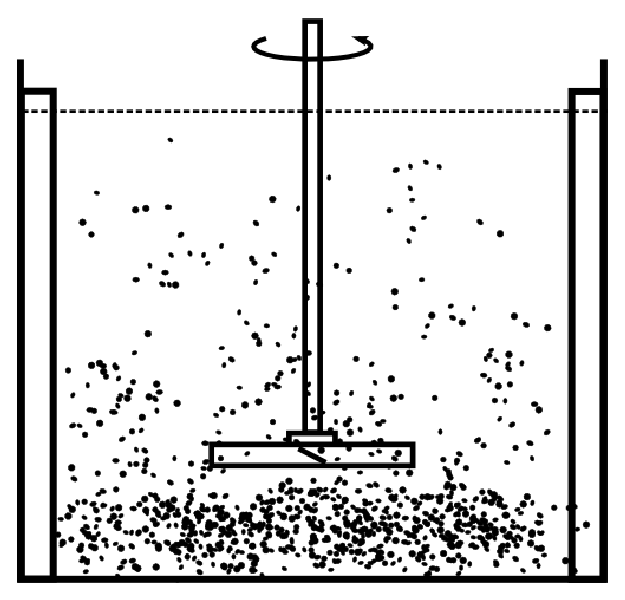
\includegraphics[scale=0.35]{images/typy_suspenzi-1.eps}}
  \qquad
  \subfloat[Úplná]{\label{fig:typ2}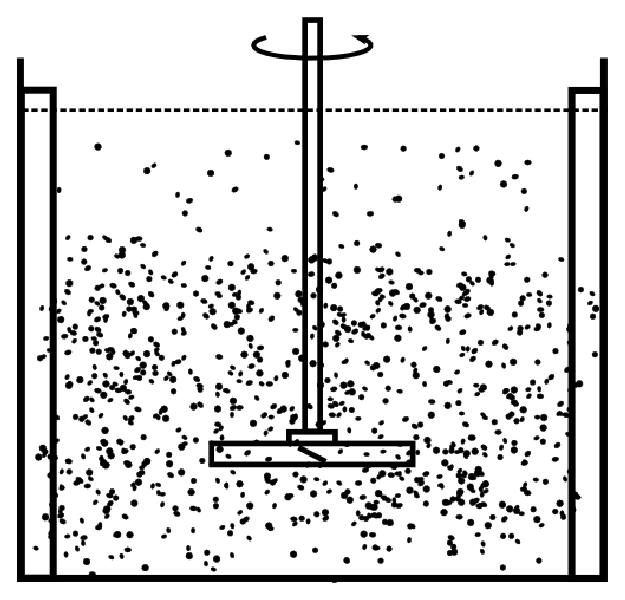
\includegraphics[scale=0.35]{images/typy_suspenzi-2.eps}}
  \qquad
  \subfloat[Homogenní]{\label{fig:typ3}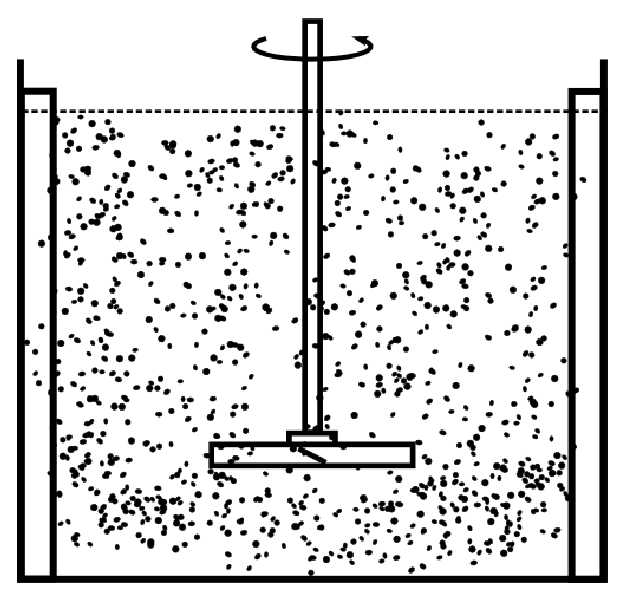
\includegraphics[scale=0.35]{images/typy_suspenzi-3.eps}}
  \caption{Stupně suspendace}
  \label{fig:typsus}
\end{figure}

Při částečné suspendaci lze vizuálně pozorovat pohyb částic pevné fáze pouze v~blízkosti dna nádoby. Toto shlukování má za následek zhoršení přestupu tepla a hmoty, což v~důsledku může snížit rychlost probíhajících chemických reakcí. Z~výše uvedeného vyplývá, že podmínky částečné suspendace jsou postačují pouze při míchaní vysoce rozpustných látek.

Stav úplné suspendace je charakterizován pohybem pevné fáze v~celé nádobě, přičemž žádná částice nezůstává na dně déle než jednu až dvě sekundy. Tato podmínka se někdy označuje jako Zwieteringovo kritérium podle autora, který jako první na základě experimentů navrhl vztah k~výpočtu kritické (minimální) frekvence otáčení míchadla potřebné k~dosažení stavu úplné suspendace. Při tomto stavu je maximální povrch částic vystaven kapalině, což má za následek intenzivní transport hmoty a tepla mezi jednotlivými fázemi.

Posledním stádiem je dosažení stavu homogenní suspendace, při němž částice pevné fáze dosahují prakticky rovnoměrného rozložení v~celém promíchávaném systému. Jakékoliv další zvýšení frekvence míchadla nebo jeho příkonu nemá již prakticky žádný vliv na distribuci pevné fáze. Dosažení stavu homogenní suspendace je často důležité u~procesů, které vyžadují rovnoměrné rozložení částic v~systému. Příkladem takovéhoto procesu může být krystalizace, kde nerovnoměrná koncentrace pevné fáze způsobuje tvorbu míst s~lokálním přesycením, jenž následně negativně ovlivňují kvalitu vzniklých krystalů. Nicméně ve většině případů je postačující dosažení stavu úplné suspendace, který vyžaduje menší množství vykonané práce.

\subsection{Kritická frekvence otáčení míchadla}
Jak již bylo zmíněno v~předcházející kapitole, kritická frekvence otáčení je minimální rychlost otáčení míchadla potřeba k~udržení částic pevné fáze ve vznosu. První kdo navrhl empirickou korelaci k~jejímu výpočtu byl \citet{zwi58}. Jím navržený vztah má tvar:
\begin{equation}
	N_{js} = \left[\frac{g(\rho_{s}-\rho_{l})}{\rho_{l}}\right]^{\num{0.45}}W^{\num{0.13}}d_{p}^{\num{0.2}}D^{\num{-0.85}}\nu^{\num{0.1}}S
	\label{eq:nkrit}
\end{equation} 
kde $g$ je gravitační zrychlení, $\rho_{s}$ hustota pevné fáze, $\rho_{l}$ hustota kapalné fáze, $W$ relativní hmotnostní zlomek pevné fáze, $d_{p}$ průměr částice pevné fáze, $\nu$ kinematická viskozita a $S$ je bezrozměrná Zwieteringova konstanta, která zohledňuje geometrii systému a míchadla (tab. \ref{tab:S}). Ze vztahu je dobře patrné, že rozdíl hustot jednotlivých fází nejvýznamněji ovlivňuje výslednou kritickou frekvenci otáčení míchadla. Později provedené studie \citep{nie68,bal78,chou97} obecně potvrdily platnost Zwieteringova vztahu. Nicméně \citet{chou97} experimentálně ukázal, že při koncentraci pevné fáze menší než \volproc{2} nebo větší než \volproc{15} se již tato korelace jeví jako nepříliš spolehlivá.

\begin{table}[h!]
\begin{center}
\caption{Zwieteringovy konstanty pro \SI{45}{\degree} PBT}
\label{tab:S}
\begin{tabular}{llr}
\toprule
\textbf{Šířka lopatky} & \textbf{Světlá výška} & \textbf{Hodnota} \\
\midrule

$D/\num{3.5}$ \\
& $T/4$ & \num{4.8} \\
& $T/6$ & \num{4.6} \\
& $T/8$ & \num{3.2} \\
$D/4$ \\
& $T/4$ & \num{4.4} \\
& $T/6$ & \num{4.1} \\
& $T/8$ & \num{3.7} \\

\bottomrule
\end{tabular}
\end{center}
\end{table}

\subsection{Kvalita suspenze (stupeň homogenizace)}
Další užitečnou charakteristikou systému kapalina-pevná fáze je takzvaná kvalita suspenze, což je směrodatná odchylka koncentrace pevné fáze. Často se však dává přednost vyjádření pomocí objemového zlomku pevné fáze. Pro konečný počet $n$ měření lze kvalitu suspenze definovat jako:
\begin{equation}
	\sigma = \sqrt{\frac{1}{n}\sum_{i=1}^{n}\left(\frac{c_{i}}{\bar{c}} - 1\right)^{2}}
	\label{eq:kvasus}
\end{equation}  

\noindent Díky své diskrétní povaze je tato veličina navíc dobře stanovitelná pomocí simulační techniky CFD. S~rostoucí homogenitou systémů číselná hodnota kvality suspenze klesá a v~limitním případě je nulová. Někdy se proto místo kvality suspenze používá pojem stupeň homogenizace, jenž vznikne odečtením kvality suspenze od jedničky.

\citet{boh80} určili na základě experimentů hodnoty kvality suspenze pro jednotlivé stupně suspendace. Jejich výsledky jsou shrnuty v~tab. \ref{tab:kvasus}.

\begin{table}[h!]
\begin{center}
\caption{Rozdělení stupňů suspendace dle kvality suspenze}
\label{tab:kvasus}
\begin{tabular}{cc}
\toprule
Stupeň suspendace & Kvalita suspenze \\
\midrule

Částečná &  $\sigma \geq \num{0.8}$ \\
Úplná & $\num{0.2} < \sigma < \num{0.8}$ \\
Homogenní & $\sigma \leq \num{0.2}$ \\

\bottomrule
\end{tabular}
\end{center}
\end{table}

\subsection{Výška vznosu pevné fáze}
Při míchaní suspenzní se ve vsádce tvoří snadno rozlišitelná oblast ve které se vyskytuje naprostá většina částic pevné fáze. Vzdálenost mezi dnem nádoby a rozhraním této oblasti se někdy také nazývá jako výška suspenzního mraku. 

Experimentálně studovali výšku suspenzního mraku např. autoři \citet{hic97}. Z~jejich měření vyplynulo, že nejvýznamnější vliv na výšku vznosu pevné fáze má poměr průměrů míchadla a nádoby $(D/T)$, poměr světlé výšky a průměru nádoby $(C/T)$ a koncentrace pevné fáze. Dosažení dobré distribuce částic ve vysoké nádobě $(H > T)$ se ukázalo jako poměrně problematické, a proto výzkumníci zdůraznili potřebu použití více míchadel v~takovýchto systémech.

\citet{bit02} odvodili korelaci pro výpočet výšky suspenzního mraku na základě dostupných experimentálních dat, které naměřili \citet{hic97} a \citet{buj99}. Zmíněný vztah byl navržen pro rychloběžná axiální míchadla a má tvar:
\begin{equation}
	C_{H}=\frac{N}{N_{js}}\left[\num{0.84} - \num{1.05}\frac{C}{T} + \num{0.7}\frac{(D/T)^{2}}{1 - (D/T)^{2}}  \right]T
	\label{eq:sushei}
\end{equation}  

\subsection{Doba homogenizace}
Doba homogenizace $t_{mix}$ je definována jako čas potřebný k tomu, aby se hodnota normalizované koncentrace stopovací látky $c(t)^{*}$ pohybovala v předem zvoleném rozmezí. Nejčastěji se volí přípustná hodnota fluktuace \SI{\pm 5}{\percent}, tedy $c(t)^{*} \in \left<\num{0.95};\num{1.05}\right>$. 

Výše zmíněná normalizovaná kocentrace je určena vztahem:
\begin{equation}
	c(t)^{*} = \frac{c(t) - c_{0}}{c_{\infty} - c_{0}}
	\label{eq:bezkon}
\end{equation}

\noindent přičemž $c(t)$ je koncentrace stopovací látky v čase $t$, $c_{\infty}$ je koncentrace ve vsádce po dokonalém rozmíchání a $c_{0}$ představuje počáteční koncentraci v systému.  

Hodnota doby homogenizace také velmi záleží na místě měření zmíněné koncentrace. Například \citet{buj99} měřili dobu homogenizace pro systém kapalina-pevná fáze v mechanicky míchané nádobě. Z výsledků vyplynulo, že nad suspenzním mrakem je doba homogenizace přibližně dvacetkrát delší než v oblasti, která je bohatá na přítomnost částic pevné fáze.

\section{Počítačová dynamika tekutin (CFD)}
Následující kapitola obsahuje stručný přehled základních rovnic a matematických modelů, které jsou uplatněny při simulaci pomocí techniky CFD. Hlavní důraz je kladen na problematiku isotermního vícefázového proudění kapalina-pevná fáze v mechanicky míchaných nádobách.

\subsection{Úvod do CFD}
Počítačová dynamika tekutin (angl. computational fluid dynamics -- CFD) je jedno z odvětví hydromechaniky, jenž využívá numerické metody a algoritmy k řešení problémů zahrnující proudění tekutin, transport hmoty a tepla, chemické reakce a celou řadu dalších fyzikálně-chemických jevů. Na počátku každé CFD simulace je třeba nejprve vytvořit model zkoumaného systémů na který jsou následně aplikovány matematické postupy tak, aby byly ze zadaných okrajových a počátečních podmínek získány vybrané údaje o dějích probíhajících v celé zkoumané doméně při respektování fyzikálních zákonů. Tyto zákony jsou nejčastěji formulovány v podobě parciálních diferenciálních rovnic. 

S prudkým nárůstem výkonu výpočetní techniky se metoda CFD stala přístupnější širšímu množství uživatelů. Mezi její hlavní výhody patří schopnost studovat systém za podmínek, kdy experimentální měření jsou těžko proveditelná, či přímo nemožná. Díky tomu je možné např. dosáhnout znatelného snížení finančních a časových nákladů ve vývojové fází nového výrobku. Nicméně je třeba dodat, že každý simulační výpočet je silně závislý na dodaných počátečních a okrajových podmínkách, a proto CFD nikdy nemůže úplně nahradit experimentální měření.

Celou CFD simulaci lze rozdělit do třech hlavních kroků: tvorba geometrie a výpočetní sítě, vlastní výpočet a analýza výsledků

\subsubsection{Tvorba geometrie a výpočetní sítě (preprocessing)}
V první fází je vytvořena geometrie zkoumaného systému, která je následně rozdělena na konečný počet kontrolních objemů (buněk). Vzniklá výpočetní síť může obsahovat buňky různých typů. Dvojrozměrná doména se nejčastěji dělí na trojúhelníky nebo obdélníky. V trojrozměrném případě se nejčastěji využívají jehlany, hranoly, kvádry či další mnohostěny. V současnosti se již dává přednost nestrukturovaným sítím před strukturovanýma. Pro strukturovanou síť platí, že každá stěna buňky přiléhá pouze k jedné stěně sousedního kontrolního objemu. Jejich hlavní nevýhodou je obtížná tvorba složitějších tvarů a nemožnost libovolného zahušťování.

\subsubsection{Vlastní výpočet}
K provedení vlastního simulačního výpočtu dnes existuje celá řada jak komerčních, tak bezplatných CFD řešičů. Příkladem komerčních produktů může být např. ANSYS Fluent, ANSYS CFX,  ANSYS Polyflow nebo STAR-CCM+. Mezi nejznámější bezplatné CFD řešiče patří OpenFOAM či Code Saturne. Interně tyto softwary využívají jednu z následujích numerických metod k řešení parciálních diferenciálních rovnic:

\begin{itemize}[itemsep=0pt,parsep=0pt,partopsep=0pt,topsep=0pt]
  \item \textbf{Metoda konečných diferencí (FDM)}
  
  Tato metoda, někdy též označována jako metoda sítí, patří mezi nejstarší techniky k řešení parciálních diferenciálních rovnic. Její podstatou je náhrada derivací pomocí diferenčních náhrad, což má za následek diskretizaci daného problému na konečný počet uzlů. Ve výsledku se tedy řeší soustava lineárních algebraických rovnic. Mezi jednu z hlavních nevýhod této metody je její obtížná formulace pro nestrukturované sítě. 
  \item \textbf{Metoda konečných objemů (FVM)}
  
  Hlavním znakem metody konečných objemů je fakt, že řeší rovnice modelu v integrální formě pro konečný počet kontrolních objemů. Díky tomu je zaručeno splnění zákonů zachování dané veličiny pro každou výpočetní buňku. Následná diskretizace výše zmíněných integrálních rovnic převádí opět vede na řešení řídké soustavy lineárních algebraických rovnic. Drtivá většina dnešních CFD rešičů využívá právě tuto numerickou metodu. 
  
  \item \textbf{Metoda konečných prvků (FEM)}
  
  Podstatou metody konečných prvků je hledání řešení daných parciálních diferenciálních rovnic v podobě po částech definovaných funkcí na předem zvoleném počtu buněk. Ve výsledku se tedy hledají váhové koeficienty pro tyto bázové funkce tak, aby získané řešení minimalizovalo chybu aproximace. Metoda konečných prvků je zvláště využívána v oblasti pevnostní analýzy nebo při simulaci proudění vysoce nenewtonovských tekutin.  
\end{itemize}

\subsubsection{Analýza výsledků (postprocessing)}
Posledním krokem každé CFD je zpracování a analýza získaných simulačních výsledků. K tomuto účelu bylo vytvořena řada softwarových nástrojů mezi které patří např. Ansys CFD-Post, Tecplot 360 nebo ParaView. Hlavní úkoly těchto programů činí:

\begin{itemize}[itemsep=0pt,parsep=0pt,partopsep=0pt,topsep=0pt]
  \item výpočet dodatečných veličin
  \item tvorba řezů doménou
  \item zobrazení vektorových polí
  \item tvorba konturových grafů
  \item vyobrazení ploch o konstantní hodnotě veličiny
  \item porovnání několika simulací
\end{itemize}

\subsection{Rovnice kontinuity}

Základní vztahem pro popis tekutiny je rovnice kontinuity, jenž vyjadřuje zákon zachování hmoty. Pro jednofázový systém obsahující stlačitelnou tekutinu má tato rovnice tvar:
\begin{equation}
	\frac{\partial \rho}{\partial t} + \nabla \cdot (\rho\vec{v}) = 0
	\label{eq:conti1}
\end{equation}
přičemž $\rho$ značí hustotu tekutiny, $t$ čas a $\vec{v}$ je vektor rychlosti. První člen v rov. \ref{eq:conti1} reprezentuje změnu hustoty v čase (akumulaci) a druhý člen představuje změnu hmotnosti objemového elementu v důsledku konvekce. Pokud lze tekutinu považovat za nestlačitelnou, tak hustota kontinua je konstantní a výše zmíněný vztah se zjednoduší na rov. \ref{eq:conti1simp}.
\begin{equation}
	\nabla \cdot \vec{v} = 0
	\label{eq:conti1simp}
\end{equation}  

\subsection{Bilance hybnosti v kontinuu}
Zákon zachování hybnosti v kontinuu je možné vyjádřit pomocí Cauchyho rovnice dynamické rovnováhy, která má tvar:
\begin{equation}
    \rho \left( \frac{\partial \vec{v}}{\partial t} + \vec{v} \cdot \nabla  \vec{v} \right) = -\nabla p +  \nabla \cdot \vec{\vec{\tau}} + \vec{f}
  	\label{eq:cauchy}
\end{equation} 
Symbol $p$ značí tlak působící na objemový element, $\vec{\vec{\tau}}$ je tenzor viskózního napětí a člen $\vec{f}$ zahrnuje další objemové síly působící na kontinuum (např. gravitační síla).

V trojrozměrné soustavě kartézských souřadnicích má tenzor viskózního napětí celkem devět složek a je definován vztahem:
\begin{equation}
    \vec{\vec{\tau}} = 
    \begin{bmatrix}
      \sigma_{xx} & \tau_{xy} & \tau_{xz}\\ 
      \tau_{yx} & \sigma_{yy} & \tau_{yz}\\ 
      \tau_{zx} & \tau_{zy} & \sigma_{zz}\\ 
    \end{bmatrix}
  	\label{eq:tenstress}
\end{equation} 
Složky napětí $\sigma_{xx}$, $\sigma_{yy}$ a $\sigma_{zz}$ působí v normálovém směru na daný objemový element a zbylé členy představují tečná napětí. Tuto skutečnost dobře ilustruje obr. \ref{fig:stresses}. 

\begin{figure}[h!]
\begin{center}
  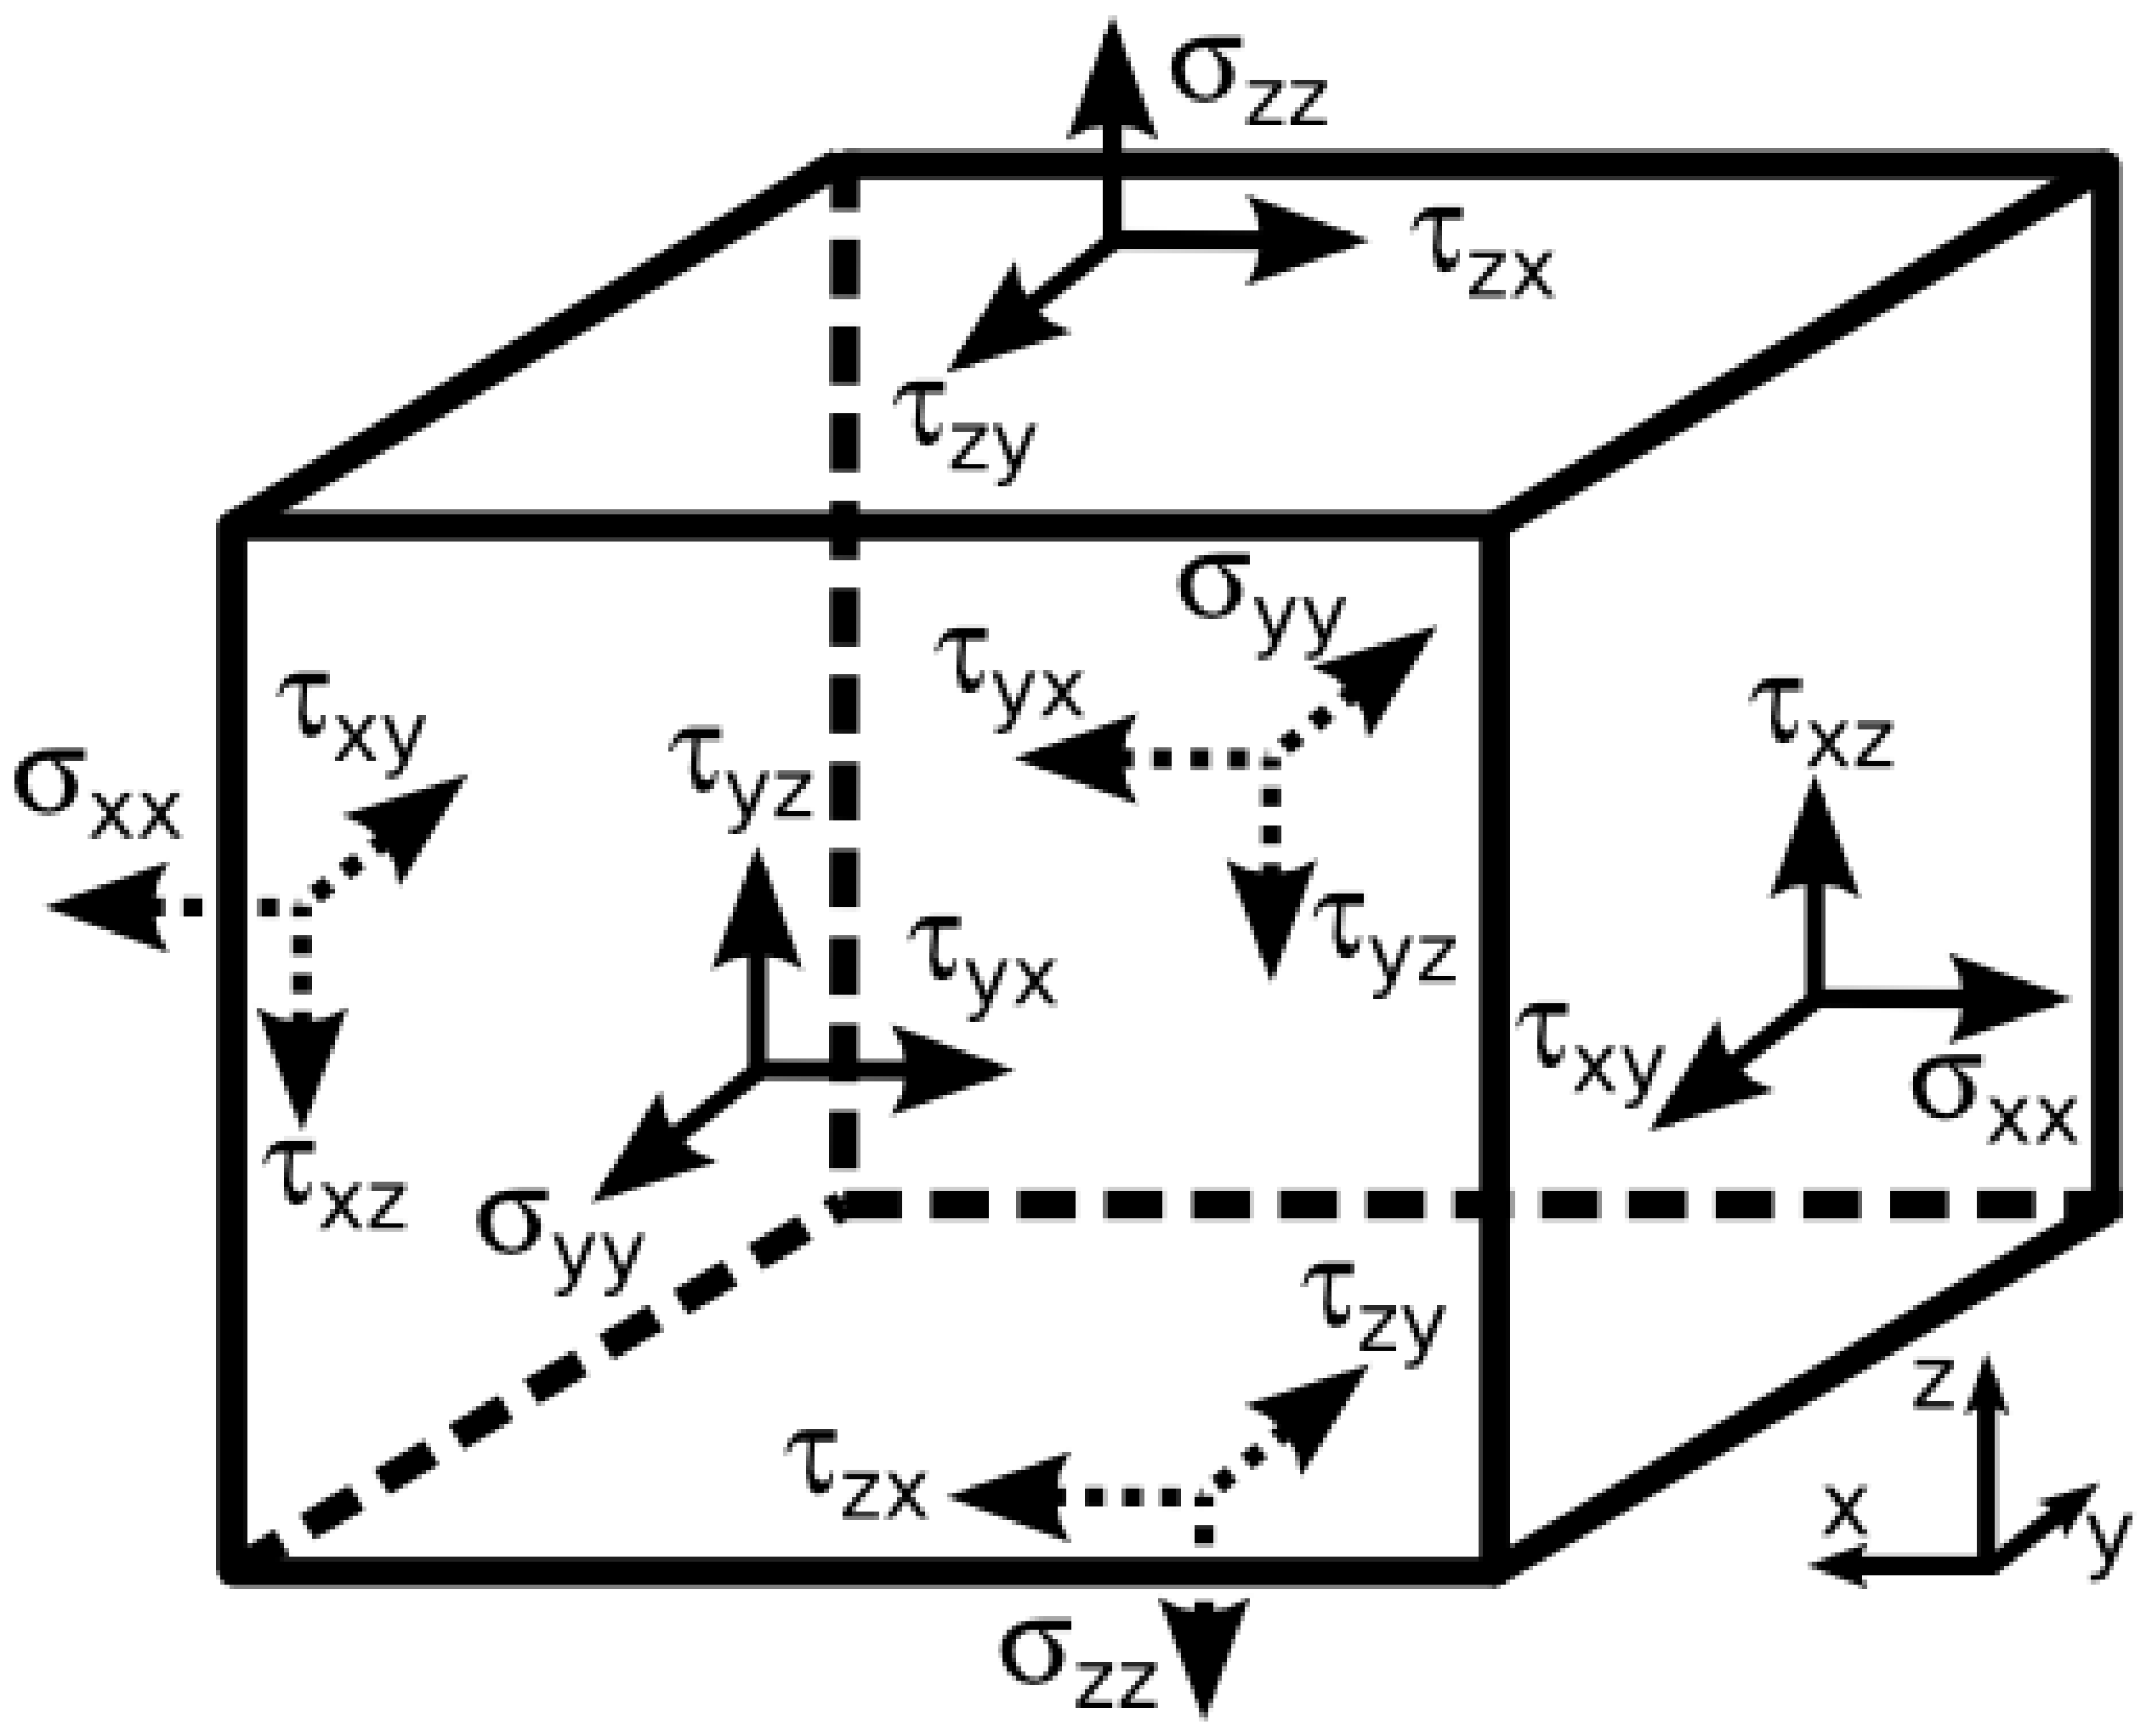
\includegraphics[scale=0.13]{images/stresses.eps}
  \caption{Složky viskózního napětí}
  \label{fig:stresses}
\end{center}
\end{figure} 

\noindent  Navíc pokud je daná tekutina izotropní (neupřednostňuje žádný směr deformace), tak tenzor \ref{eq:tenstress} má pouze šest nezávislých složek, protože mezi tečnými napětími platí vztahy:
\begin{equation}
    \begin{array}{ccc}
      \tau_{xy} = \tau_{yx}, & \tau_{xz} = \tau_{zx}, & \tau_{zy} = \tau_{yz}
      \end{array}
  	\label{eq:dept}
\end{equation} 
Pro Newtonovskou tekutinu dále platí, že jednotlivá viskózní napětí jsou úměrná míře lineárních deformací objemového elementu kontinua. Tenzor \ref{eq:tenstress} lze poté vyjádřit jako: 
\begin{equation}
    \vec{\vec{\tau}} = 
    \begin{bmatrix}
      2\eta\frac{\partial v_{x}}{\partial x} + \left( \kappa - \frac{2}{3} \eta  \right)  \nabla \cdot \vec{v} & \eta \left( \frac{\partial v_{x}}{\partial y} + \frac{\partial v_{y}}{\partial x} \right) & \eta \left( \frac{\partial v_{x}}{\partial z} + \frac{\partial v_{z}}{\partial x} \right)\\ 
      \eta \left( \frac{\partial v_{x}}{\partial y} + \frac{\partial v_{y}}{\partial x} \right) & 2\eta\frac{\partial v_{y}}{\partial y} + \left( \kappa - \frac{2}{3} \eta  \right)  \nabla \cdot \vec{v} 
      & \eta \left( \frac{\partial v_{y}}{\partial z} + \frac{\partial v_{z}}{\partial y} \right)\\ 
      \eta \left( \frac{\partial v_{x}}{\partial z} + \frac{\partial v_{z}}{\partial x} \right) & \eta \left( \frac{\partial v_{y}}{\partial z} + \frac{\partial v_{z}}{\partial y} \right)
      & 2\eta\frac{\partial v_{z}}{\partial z} + \left( \kappa - \frac{2}{3} \eta  \right) \nabla \cdot \vec{v}\\ 
    \end{bmatrix}
  	\label{eq:newtenstress}
\end{equation} 
Člen $\eta$ představuje dynamickou (tečnou) viskozitu a $\kappa$ značí dilatační (objemovou) viskozitu, jejíž hodnota je nulová pro jednoatomové plyny při nízké hustotě. Někdy se tenzor \ref{eq:newtenstress} zapisuje v úspornější podobě:
\begin{equation}
	\vec{\vec{\tau}} = \eta \left[ \nabla \vec{v} +  \left( \nabla \vec{v} \right)^{\mathsf{T}}\right] +  \left( \kappa -\frac{2}{3} \eta \right) \nabla \cdot \vec{v} \vec{\vec{I}}
	\label{eq:comptenstress}
\end{equation}
kde $\vec{\vec{I}}$ je jednotkový tenzor.

Dosazením vztahu \ref{eq:comptenstress} do rov. \ref{eq:cauchy} a při předpokladu nestlačitelnosti kontinua ($\nabla \cdot \vec{v} = 0$) se získá Navierova-Stokesova rovnice:
\begin{equation}
    \rho \left( \frac{\partial \vec{v}}{\partial t} + \vec{v} \cdot \nabla  \vec{v} \right) = -\nabla p + \eta \nabla^{2}\vec{v}  + \vec{f}
  	\label{eq:navst}
\end{equation} 
Ve trojrozměrné soustavě kartézských souřadnic lze vektorovou rov. \ref{eq:navst} rozepsat na 
\begin{equation}
\begin{array}{c}
    \rho \left( \frac{\partial v_{x}}{\partial t} + v_{x}\frac{\partial v_{x}}{\partial x} + v_{y}\frac{\partial v_{x}}{\partial y} + v_{z}\frac{\partial v_{x}}{\partial z} \right) = -\frac{\partial p}{\partial x} +  \eta \left( \frac{\partial^{2} v_{x}}{\partial x^{2}} + \frac{\partial^{2} v_{y}}{\partial y^{2}} + \frac{\partial^{2} v_{z}}{\partial z^{2}} \right) + f_{x}   \vspace{3mm} \\
    
    \rho \left( \frac{\partial v_{y}}{\partial t} + v_{x}\frac{\partial v_{y}}{\partial x} + v_{y}\frac{\partial v_{y}}{\partial y} + v_{z}\frac{\partial v_{y}}{\partial z} \right) = -\frac{\partial p}{\partial y} +  \eta \left( \frac{\partial^{2} v_{x}}{\partial x^{2}} + \frac{\partial^{2} v_{y}}{\partial y^{2}} + \frac{\partial^{2} v_{z}}{\partial z^{2}} \right) + f_{y}   \vspace{3mm} \\
    
    \rho \left( \frac{\partial v_{z}}{\partial t} + v_{x}\frac{\partial v_{z}}{\partial x} + v_{y}\frac{\partial v_{z}}{\partial y} + v_{z}\frac{\partial v_{z}}{\partial z} \right) = -\frac{\partial p}{\partial z} +  \eta \left( \frac{\partial^{2} v_{x}}{\partial x^{2}} + \frac{\partial^{2} v_{y}}{\partial y^{2}} + \frac{\partial^{2} v_{z}}{\partial z^{2}} \right) + f_{z}   \\
    \end{array}
  	\label{eq:navst3d}
\end{equation} 
Soustava rovnic \ref{eq:navst3d} spolu s rov. \ref{eq:conti1simp} tvoří systém čtyř parciálních diferenciálních rovnic pro neznámé $p$, $v_{x}$, $v_{y}$ a $v_{z}$. 

\subsection{Vícefázové modely}
Velké množství přírodních a průmyslových procesů je tvořeno vícefázovým prouděním. Problematika simulace tohoto děje je daleko komplexnější než v případě systému složeného pouze z jedné fáze. V hydrodynamice je pojem fáze chápán v širším smyslu než z termodynamického hlediska. Z tohoto pohledu lze fází definovat jako třídu materiálu, jenž interaguje určitým způsobem s dalšími částmi systému. 

V~současnosti existuje řada matematických modelů, které popisují vícefázové proudění a lišící se výsledným způsobem použití. Následující podkapitola obsahuje přehled modelů, které se nejčastěji využívají k~simulaci suspendace v~mechanicky míchaných nádobách. Především se jedná o simulační techniky Eulerian-Lagrangian, Eulerian-Eulerian a Eulerian-Granular.

\subsubsection{Model Eulerian-Lagrangian}
Tento typ modelu uvažuje primární tekutou fází jako kontinuum s~dispergovanou sekundární fází. Pro primární fázi je řešena rovnice kontinuity (\ref{eq:conti1simp}) spolu s~Navierovými-Stokesovými rovnicemi (\ref{eq:navst3d}), zatímco pro dispergovanou fázi je řešena trajektorie každé částice nebo skupiny částic separátně. Jednotlivé fáze si mohou mezi sebou vyměňovat hmotu, hybnost a energii, avšak vzájemné interakce částic mezi sebou jsou většinou zanedbány. Model Eulerian-Lagrangian je především vhodný pro systémy, kde objemový zlomek dispergované fáze nepřesáhne \SI{10}{\percent} např: rozprašovací sušárny, cyklóny nebo spalování uhlí či kapalného paliva. 

Řešením bilance sil působící na částici (rov. \ref{eq:dpm}) je získána její trajektorie v~daném časovém okamžiku.
\begin{equation}
	m_{p}\od{\vec{v}_{p}}{t} = \vec{F}_{p} + \vec{F}_{g} + \vec{F}_{B} + \vec{F}_{D} + \vec{F}_{ad}
	\label{eq:dpm}
\end{equation} 
Členy $m_{p}$ a $\vec{v}_{p}$ na levé straně rov. \ref{eq:dpm} představují hmotnost částice a její vektor rychlosti. Pravá strana výše zmíněné rovnice obsahuje součet jednotlivých sil působících na diskrétní fázi. Symbol $\vec{F}_{p}$ značí sílu tlakového gradientu, jenž působí na částici vlivem akcelerace okolní kapaliny. Další členy $\vec{F}_{g}$ a $\vec{F}_{B}$ reprezentují gravitační resp. vztlakovou sílu. Jednotlivé příspěvky těchto sil lze rozepsat do tvaru:    
\begin{equation}
	\vec{F}_{p} + \vec{F}_{g} + \vec{F}_{B} = V_{p} \nabla p + m_{p} \vec{g} -  V_{p} \rho_{f} \vec{g}
	\label{eq:force3}
\end{equation} 
 Odporová síla $\vec{F}_{D}$ představuje výslednici sil kterou tekutina působí proti pohybu částic. Pro kulovou částici lze tento člen vyjádřit jako:
\begin{equation}
	\vec{F}_{D} = \frac{\pi}{8}C_{D}\rho_{f} d_{p}^{2} \left|\vec{v}_{p} - \vec{v}_{f}\right| \left(\vec{v}_{p} - \vec{v}_{f}\right)
	\label{eq:fd}
\end{equation} 
Bezrozměrné číslo $C_{D}$ v rov. \ref{eq:fd} se nazývá koeficient odporu nebo součinitel tření a vyjadřuje závislost odporu prostření na tvaru tělesa, charakteru proudění a vlastnostech tekutiny. Detailnějším rozborem tohoto členu se zabývá kapitola XXX.

Poslední příspěvkem $\vec{F}_{ad}$ do bilance \ref{eq:dpm} zahrnuje další síly působící na částici pevné fáze. Jedná se například o Saffmanovu vztlakovou sílu, jenž vzniká v důsledku vířivosti rychlostního pole kapalné fáze a působí především na částice o velikosti menší než několik mikrometrů. Další silou která se někdy zohledňuje při vícefázové simulaci je zdánlivá setrvačná síla, která je způsobena společným pohybem tekutiny v blízkosti dispergované fáze při její akceleraci. Tento jev má za následek dočasný zdánlivý nárůst hmotnosti částic. Zdánlivá setrvačná síla se projevuje především v systémech kapalina-plynná fáze.  

\subsubsection{Model Eulerian-Eulerian}
U~modelu Eulerian-Eulerian jsou jednotlivé fáze považovány za prostupující se kontinua a každý bod v~systému obsahuje informaci o~objemovém zlomku dané fáze. Z~tohoto popisu je zřejmé, že suma objemových zlomků přes všechny fáze v~libovolném bodě se vždy musí rovnat jedné. 
\begin{equation}
	\sum_{i=1}^n \alpha_{i} = 1
	\label{eq:volfrac}
\end{equation} 

Jednotlivé fáze mohou být kapalné, plynné nebo pevné a jejich celkový počet není teoreticky limitován. Pro každou fázi se řeší rovnice kontinuity a sada rovnic pro hybnost. K~výměně hybnosti mezi jednotlivými fázemi slouží mezifázové členy v~těchto rovnicích. Pokud dochází k~přenosu tepla nebo hmoty je třeba tuto skutečnost zohlednit v~bilanci energie a hmoty.    

Pro vícefázový systém je třeba zapsat rovnici kontinuity pro každou fázi zvlášť, přičemž je třeba obecně uvažovat přenos hmoty mezi jednotlivými fázemi. Rovnice kontinuity pro $i$-tou fázi lze zapsat jako:
\begin{equation}
	\frac{\partial}{\partial t} (\alpha_{i}\rho_{i}) +  \nabla \cdot (\alpha_{i}\rho_{i}\vec{v}_{i}) = \sum_{\substack{ i \neq j \\ j=1}}^{n}\Gamma_{ij}
	\label{eq:conti2}
\end{equation} 
kde člen $\Gamma_{ij}$ představuje hmotnostní tok mezi $i$-tou a $j$-tou fází vztažený na objemový element a $\alpha_{i}$ značí objemový zlomek dané fáze. Pokud však nedochází k transportu hmoty mezi fázemi, tak se rov. \ref{eq:conti2} zjednoduší do tvaru:
\begin{equation}
	\frac{\partial}{\partial t} (\alpha_{i}\rho_{i}) +  \nabla \cdot (\alpha_{i}\rho_{i}\vec{v}_{i}) = 0
	\label{eq:conti3}
\end{equation} 

Rovnice hybnosti pro $i$-tou fázi za předpokladu nulového mezifázového transportu hmoty lze zapsat jako:
\begin{equation}
	\frac{\partial}{\partial t} \left(\alpha_{i}\rho_{i}\vec{v}_{i}\right) + \nabla \cdot (\alpha_{i}\rho_{i} \vec{v}_{i} \otimes \vec{v}_{i}) = -\alpha_{i} \nabla p + \nabla \cdot \left(\alpha_{i} \vec{\vec{\tau}}_{i} \right) +\sum_{\substack{ i \neq j \\ j=1}}^{n} \vec{R}_{ji} + \vec{f}_{ext,i} + \vec{f}_{int,i}
	\label{eq:moml}
\end{equation}
\noindent kde $p$ je tlak sdílený mezi všemi fázemi, $\vec{\vec{\tau}}_{i}$ je tenzor viskózního napětí, jehož konkretní tvar závisí na typu uvažované fáze. Člen $\vec{R}_{ji}$ představuje mezifázovou odporovou sílu mezi $i$-tou a $j$-tou fází, $\vec{f}_{ext,i}$ má význam dalších objemových sil a $\vec{f}_{int,i}$ zahrnuje povrchové síly působící na $i$-tou fázi vlivem ostatních fází. Všechny výše zmíněné síly jsou vztaženy na objemový element dané fáze. 

Člen mezifázové odporové síly $\vec{R}_{ji}$ v~rovnici \ref{eq:moml} nejvýznamněji přispívá do popisu interakce mezi jednotlivými fázemi, a proto správnost popisu tohoto členu zásadně ovlivňuje kvalitu výsledné simulace. Tuto sílu lze rozepsat jakou součin koeficientu mezifázového sdílení hybnosti a relativní rychlosti $i$-té a $j$-té fáze.
\begin{equation}
	 \sum_{\substack{ i \neq j \\ j=1}}^{n} \vec{R}_{ji} = K_{ji} \left( \vec{v}_{j} - \vec{v}_{i} \right)
	\label{eq:kij}
\end{equation}
Z~definice \ref{eq:kij} je jasné, že platí vztah $\vec{R}_{ji} = -\vec{R}_{ij}$. Vzorec pro výpočet $K_{ji}$ se obecně liší podle toho jaké typy fází spolu interagují. Pokud se jedná o~interakci kapalina-pevná fáze, tak koeficient mezifázového sdílení hybnosti má tvar:
\begin{equation}
	K_{fs}= \frac{3\alpha_{s}C_{D}\rho_{f}\left|\vec{v}_{s} - \vec{v}_{f}\right|}{4d_{s}}
	\label{eq:kfs}
\end{equation}
Symbol $d_{s}$ značí průměr částic pevné fáze a $C_{D}$ je koeficient odpor, kterým se právě ovlivňuje chování odporové síly. 
 
Za zmínku stojí fakt, že při využití modelu Eulerian-Eulerian se pevná fáze modeluje jako kapalina bez vnitřního tření. Rigoróznější popis pevné fáze přináší až model Eulerian-Granular, který je diskutovaný níže. 

\subsubsection{Model Eulerian-Granular}
\label{sec:egm}
Vícefázový model Eulerian-Granular se liší od předchozího tím, že  popis chování pevné fáze byl odvozen s~využitím kinetické teorie, která je například známá ze statistického popisu plynů. U~tohoto modelu se viskozita pevné fáze mění v~závislosti na interakcích s~ostatními částicemi a primární fází. Mezi nejčastější aplikace patří simulace fluidních loží nebo suspendace v~mechanicky míchaných nádobách.

Bilanci hybnosti pro pevnou fázi $s$ má tvar:
\begin{equation}
	\frac{\partial}{\partial t} \left(\alpha_{s}\rho_{s}\vec{v}_{s}\right) + \nabla \cdot (\alpha_{s}\rho_{s} \vec{v}_{s} \otimes \vec{v}_{s}) = -\alpha_{s} \nabla p - \nabla p_{s} + \nabla \cdot \left(\alpha_{s} \vec{\vec{\tau}}_{s} \right) +\sum_{\substack{ j \neq s \\ j=1}}^{n} \vec{R}_{ji} + \vec{f}_{ext,s} + \vec{f}_{int,s}
	\label{eq:moms}
\end{equation}
Člen $p_{s}$ je tlak pevné fáze, který se skládá z kinetické části a členu, který výsledkem neelastických srážek mezi částicemi. V současnosti existuje řada modelů k výpočtu tlaku pevné fáze. Jedním z nich je model odvozený autory \citet{lun84}:
\begin{equation}
	p_{s} = \alpha_{s}\rho_{s}\Theta + 2\rho_{s}\left(1 + r_{s} \right) \alpha_{s}^{2}g_{s}\Theta
	\label{eq:ps}
\end{equation}
kde $r_{s}$ je restituční koeficient vyjadřující míru elasticity srážek mezi částicemi. Symbol $g_{s}$ představuje radiální distribuční funkci, jenž upravuje pravděpodobnost kolizí částic pevné fáze. Poslední nediskutovaným členem $\Theta$ je teplota zrnité fáze, která je úměrná velikosti střední kvadratické rychlosti náhodného pohybu částic, tedy: 
\begin{equation}
	\Theta = \frac{1}{3} \overline{ \vec{u} \cdot \vec{u}}
	\label{eq:gtemp}
\end{equation}
Ve většině CFD řešíčů se určení hodnoty teploty zrnité fáze využívají algebraické modely odvozené z transportní rovnice pro tuto veličinu.

Tenzor viskózního napětí pevné fáze $\vec{\vec{\tau}}_{s}$ v rov. \ref{eq:moms} lze vyjádřit formálně stejně jako ve vztahu \ref{eq:comptenstress}. 
\begin{equation}
	\vec{\vec{\tau_{s}}} = \eta_{s} \left[ \nabla \vec{v_{s}} +  \left( \nabla \vec{v_{s}} \right)^{\mathsf{T}}\right] +  \left( \kappa_{s} -\frac{2}{3} \eta_{s} \right) \nabla \cdot \vec{v_{s}} \vec{\vec{I}}
	\label{eq:solidstress}
\end{equation}
Tečná viskozita zrnité fáze $\eta_{s}$ je dána součtem kolizní, kinetické a frikční části:
\begin{equation}
	\eta_{s} = \eta_{s,col}  + \eta_{s,kin} + \eta_{s,fr} 
	\label{eq:nys}
\end{equation}
přičemž běžně využívané korelace k jejich určení byly navrženy \citet{gid92}, \citet{syam93}. Dilatační viskozita $\kappa_{s}$ zohledňuje odpor pevných částic při expanzi či kompresi. \citet{lun84} odvodili následující vztah k jejímu výpočtu:
\begin{equation}
	\kappa_{s} = \frac{4}{3}\alpha_{s}\rho_{s}d_{s}g_{s}\left(1 + r_{s} \right)\sqrt{\frac{\Theta}{\pi}}
	\label{eq:dilvis}
\end{equation}
 
\subsection{Koeficient odporu}
Koeficient odporu (součinitel tření) má zásadní vliv na velikost a charakter mezifázové odporové síly. Obecně je tento člen funkcí relativní rychlosti pohybu částic, jejich velikostí, hustotou a viskozitou tekutiny či případně dalších veličin. V~současnosti existuje celá řada modelů pro koeficient odporu, které se liší podle toho pro jaký účel byly navrženy. V této kapitole jsou především uvedeny korelace, jenž se používají při simulacích systému kapalina-pevná fáze v míchaných nádobách. 

Jeden z nejznámějších modelů k výpočtu součinitele tření navrhli \citet{schi32}, kteří získali vztah \ref{eq:schlneu} pro výpočet koeficientu odporu na základě experimentálního měření rychlosti usazování sférické částice ve stagnantním sloupci kapaliny.    
\begin{equation}
	\label{eq:schlneu}
  C_{D0} = \left\{ \begin{array}{ll}
  \frac{24}{Re_{p}}  \left( 1 + \num{0.15}Re_{p}^{\num{0.687}} \right) & Re_{p} \le 1000\\
  \num{0.44} & Re_{p} > 1000\\
  \end{array} \right.
\end{equation}
\noindent Ze vztahu \ref{eq:schlneu} je patrné, že Schillerova-Naumannova korelace je funkcí Reynoldsova kritéria pro částici které je definováno jako:
\begin{equation}
	Re_{p}= \frac{\rho_{f}d_{s}\left|\vec{v}_{s} - \vec{v}_{f}\right|}{\eta_{f}}
	\label{eq:reyp}
\end{equation}

Bohužel koeficient odporu navržený Schillerem a Naumannem se ukázal jako nepříliš vhodný k~popisu odporové síly v~systémech s~plně vyvinutým turbulentním prouděním, a proto řada autorů se zaměřila na úpravu této korelace.

\citet{bru98} měřili rychlost usazování pevné fáze mezi dvěma opačně rotujícími válci (Taylorův–Couettův tok). Ze získaných výsledků následně autoři stanovili korelaci pro koeficient odporu zohledňující volnou turbulenci. Naproti tomu \citet{pin01} odvodili model pro koeficient odporu na základě experimentální studie suspendace v nádobě osazené skupinou míchadel. \citet{kho06} upravili Brucátův vztah na základě srovnání experimentálních a simulačních výsledků získaných pomocí CFD během studie suspendace v míchané nádobě. 

Všechny výše zmíněné korelace jsou uvedeny v~tab. \ref{tab:cds}. Člen $\lambda$ se nazývá Kolmogorovo mikroměřítko a určuje nejmenší velikost turbulentní vírů přítomných v~systému, přičemž je funkcí kinematické viskozity tekutiny a rychlostí disipace turbulentní kinetické energie (viz. rov.).
\begin{equation}
  \lambda = \left( \frac{\nu^{3}}{\epsilon} \right) ^{1/4}
	\label{eq:kolmo}
\end{equation}

\begin{table}[h!]
\begin{center}
\caption{Modely pro odporový koeficient v~turbulentní oblasti proudění}
\label{tab:cds}
\begin{tabular}{cc>{\centering\arraybackslash}p{5cm}}
\toprule
\textbf{Autor} & \textbf{Koeficient odporu} & \textbf{Stanoveno na základě} \\
\midrule{}

\multirow{2}{*}{\citet{bru98}} & \multirow{2}{*}{$C_{D} = C_{D0} \left[ 1 + \num{8.76e-4} \left( \frac{\lambda}{d_{s}} \right)^{3} \right] $} & experimentální studie Taylorova–Couettova toku \\ \addlinespace

\multirow{2}{*}{\citet{pin01}} & \multirow{2}{*}{$C_{D} = C_{D0} \left[ \num{0.4}\tanh\left(  \frac{16\lambda}{d_{s}} - 1  \right) \right] ^{-2}$} & měření rychlosti usazování v~míchací nádobě \\ \addlinespace

\multirow{2}{*}{\citet{kho06}} & \multirow{2}{*}{$C_{D} = C_{D0} \left[ 1 + \num{8.76e-5} \left( \frac{\lambda}{d_{s}} \right)^{3} \right]$} & úpravy Brucatova vztahu pro míchací nádoby  \\

\bottomrule
\end{tabular}
\end{center}
\end{table}

\subsection{Turbulentní modely}
Turbulentní pohyb patří k nejsložitějším a současně nejběžnějším přírodním jevům pozorovaných v proudících tekutinách. Z tohoto důvod je turbulenci věnována mimořádná pozornost v technických aplikacích zabývající se dynamikou proudění. 

Proudění v tekutinách lze obecně rozdělit na dva hlavní typy: laminární a turbulentní. Při laminárním proudění jsou jednotlivé proudnice tekutiny spolu rovnoběžné a k promíchávání prakticky nedochází. Naproti tomu pro turbulentní proudění je charakteristické intenzivní promíchávání a vysoká míra neuspořádanosti probíhajícího procesu. Významný je také fakt, že mezi laminárním a turbulentním charakterem toku se ještě vyskytuje tzv. přechodové proudění jehož teoretický popis je velmi obtížný. Pro kvalitativní posouzení charakteru proudění se využívá Reynoldsovo číslo ($Re$), které je řádově vyšší v turbulentní oblasti než v laminární. 

Z pohledu numerické simulace existují tři hlavní směry, jak se vypořádat s popisem toku tekutiny v turbulentní oblasti proudění. Jedná se o:
\begin{itemize}[itemsep=0pt,parsep=0pt,partopsep=0pt,topsep=0pt]
  \item přímou numerickou simulaci (DNS)
  \item časově zprůměrované Navierovy-Stokesy rovnice (RANS)
  \item techniku velkých vírů (LES)
\end{itemize}

\paragraph{Přímá numerická simulaci (DNS)}
Následující přístup řeší k určení proudového pole pouze rovnici kontinuity a Navierovy-Stokesovy rovnice bez využití dodatečných rovnic pro turbulenci. Toto znamená, že celá škála prostorových a časových měřítek musí být řešena přímo, a proto použitá výpočetní doména musí být dostatečně jemná. Počet potřebný buněk obsažených ve výpočetní sítí roste přibližně kvadraticky s hodnotou Reynoldsova čísla ($Re^{3/4}$). Z tohoto důvodu klade technika DNS značné nároky na výpočetní techniku a následné vyhodnocení.

\paragraph{Technika velkých vírů (LES)}
Metoda LES představuje kompromis mezi přímou numerickou simulací (DNS) a časovým zprůměrováním Navierových-Stokesových rovnic (RANS). Tato technika je založena na hypotéze, že měřítka turbulentního proudění mohou být rozděleny na velkou a malou (podsíťovou) složku. Velké víry, jakožto hlavní nositelé kinetické energie, jsou řešený přímo zatímco malé víry jsou modelovány. Klíčovým krokem metody je filtrování Navierových-Stokesových rovnic, což vede k odstranění malých prostorových a časových měřítek z výsledného řešení. Intenzita filtrování přímo ovlivňuje míru získaných detailů proudového pole a tedy časovou náročnost simulace. Bohužel tato technika není implementována v současných CFD řešičích 
Metoda LES představuje kompromis mezi přímou numerickou simulací (DNS) a časovým zprůměrováním Navierových-Stokesových rovnic (RANS). Tato technika je založena na hypotéze, že měřítka turbulentního proudění mohou být rozděleny na velkou a malou (podsíťovou) složku. Velké víry, jakožto hlavní nositelé kinetické energie, jsou řešený přímo zatímco malé víry jsou modelovány. Klíčovým krokem metody je filtrování Navierových-Stokesových rovnic, což vede k odstranění malých prostorových a časových měřítek z výsledného řešení. Intenzita filtrování přímo ovlivňuje míru získaných detailů o proudovém poli a tedy časovou náročnost simulace. Bohužel tato technika není v současnosti implementována běžnými CFD řešiči pro využití ve vícefázových simulacích. 

\paragraph{Časově zprůměrované Navierovy-Stokesy rovnice (RANS)}
Principem metody RANS je rozložení okamžité hodnoty veličiny popisující proudění na složku časově zprůměrovanou a fluktuační, tedy:
\begin{equation}
  \phi = \avg{\phi} + \phi'
  \label{eq:avg_vels}
\end{equation}
Přičemž časově zprůměrovaná veličina je definovaná jako:
\begin{equation}
  \avg{\phi}  = \frac{1}{\bigtriangleup t} \int_{t_{0}}^{t_{0} + \bigtriangleup t} \phi\,\mathrm{d}t
  \label{eq:phi_avg}
\end{equation}
Dosazením vztahu \ref{eq:avg_vels} do rov. \ref{eq:cauchy} pro nestlačitelnou tekutinu se získá Reynoldsova zprůměrovaná bilance hybnosti:  
\begin{equation}
    \rho \left( \frac{\partial \avg{\vec{v}}}{\partial t} + \avg{\vec{v}} \cdot \nabla  \avg{\vec{v}} \right) = -\nabla \avg{p} +  \nabla \cdot \avg{\vec{\vec{\tau}}} + \vec{\vec{\tau}}_{R} + \avg{\vec{f}}
  	\label{eq:cauchy_avg}
\end{equation} 
kde $\vec{\vec{\tau}}_{R}$ je tenzor Reynoldsova napětí mající členy: 
\begin{equation}
    \begin{array}{cc}
      \tau_{R,ij} = -\rho\avg{v_{i}'v_{j}'}, & \sigma_{R,ii} = -\rho\avg{\left(v_{i}'\right)^{2}}
      \end{array}
      \label{eq:rey_stress}
\end{equation}
Obdobným způsobem lze odvodit časově zprůměrovanou rovnici kontinuity pro nestlačitelnou tekutinu.
\begin{equation}
	\nabla \cdot \avg{\vec{v}} = 0
	\label{eq:conti1simp_avg}
\end{equation}  

Díky časovému zprůměrování jsou malá prostorová a časová měřítka vyhlazena, a proto tato technika je méně výpočetně náročná než DNS nebo LES přístupy. Nicméně RANS technika zavádí nové neznámé proměnné (složky Reynoldsova napětí), které je potřeba vhodně určit. K jejich stanovení se zavádějí aproximace a předpoklady označované jako turbulentní modely. Mezi nejznámější představitele těchto modelů patří: 
\begin{itemize}[itemsep=0pt,parsep=0pt,partopsep=0pt,topsep=0pt]
  \item Spalart-Allmaras (1 rovnice) 
  \item \keps{} (2 rovnice) 
  \item \komg{} (2 rovnice) 
  \item Reynoldsův napěťový model (7 rovnice)
\end{itemize}
Velká část turbulentních modelů (např. první tři ve výše uvedeném výčtu) je založena na tzv. Boussineqově hypotéze XXX, která modeluje složky Reynoldsova napětí pomocí gradientů rychlosti a skalární veličiny nazývané turbulentní viskozita ($\eta_{t}$). Členy ve vztahu \ref{eq:rey_stress} lze poté rozepsat jako: 
\begin{equation}
    \begin{array}{cc}
      \tau_{R,ij} = \eta_{t}\left( \pd{v_{i}}{x_{j}} + \pd{v_{j}}{x_{i}} \right), & \sigma_{R,ii} = 2\eta_{t}\pd{v_{i}}{x_{i}}  - \frac{2}{3} \left[ \rho k + \eta_{t} \left( \nabla  \cdot \vec{v} \right) \right]
      \end{array}
      \label{eq:rey_stress_bus}
\end{equation}
kde $k$ je turbulentní kinetická energie. Jednou z výhod toto přístupu je relativně nízká výpočetní náročnost k určení turbulentní viskozity. Naopak mezi jeho hlavní nevýhody patří předpoklad isotropní turbulence, který nemusí být v řadě případů splněn.  

\subsubsection{Standardní \kepsb{} turbulentní model pro směs}
Tento model představuje první typ rozšíření klasického \keps{} pro jednofázový tok. Jeho použití je především vhodné v případech kdy poměr hustot jednotlivých fází je blízký jedničce. V takových to případech k popisu turbulentního proudu stačí využít veličiny popisující celou směs. Hustota směsi a vektor rychlosti směsi je vypočtena podle vztahu \ref{eq:rho_m} resp. \ref{eq:vel_m}.
\begin{equation}
	\rho_{m} = \sum_{i=1}^n \alpha_{i}\rho_{i}
	\label{eq:rho_m}
\end{equation}  
\begin{equation}
	\vec{v}_{m} = \frac{\sum_{i=1}^n \alpha_{i}\rho_{i}\vec{v}_{i}}{\rho_{m} }
	\label{eq:vel_m}
\end{equation}  
Turbulentní viskozita je vypočtena ze vztahu:
\begin{equation}
	\eta_{t} = \rho_{m}C_{\eta}\frac{k^{2}}{\epsilon}
	\label{eq:turb}
\end{equation}  
přičemž hodnoty veličin $k$ a $\epsilon$ jsou získány řešením příslušných transportních rovnic \ref{eq:k-eq} a \ref{eq:eps-eq}.
\begin{equation}
	\pd{\rho_{m}k}{t} +  \nabla  \cdot \left( \rho_{m} \vec{v}_{m} k \right) = \nabla  \cdot \left( \frac{\eta_{t}}{\sigma_{k}} \nabla k \right) + G_{k} - \rho_{m}\epsilon
	\label{eq:k-eq}
\end{equation}  
\begin{equation}
	\pd{\rho_{m}\epsilon}{t} +  \nabla  \cdot \left( \rho_{m} \vec{v}_{m} \epsilon \right) = \nabla  \cdot \left( \frac{\eta_{t}}{\sigma_{\epsilon}} \nabla \epsilon \right) + \frac{\epsilon}{k} \left( C_{1\epsilon}G_{k} - C_{2\epsilon}\rho_{m}\epsilon \right)
	\label{eq:eps-eq}
\end{equation}  

	\chapter{Literární rešerše}
Suspendace pevné fáze v mechanicky míchaných nádobách patří v posledních desetiletích ke značně studovanému jevu. Za průkopníka v této oblasti je označován \citet{zwi58}, jenž vyvinul empirickou korelaci pro výpočet frekvence otáčení míchadla při které již dochází ke vznosu částic. Při této frekvenci žádná částice nezůstává na dně nádoby déle než jednu či dvě sekundy. Také další autoři intenzivně experimentálně studovali mechanizmus suspendace v promíchávaných nádobách \citep{nie68,bal78,arm98}. 

V posledních třech dekádách mnoho výzkumníků obrátilo svoji pozornost k počítačové dynamice tekutin jako k prostředku ke zkoumání procesů probíhajících ve vícefázových systémech. Od té doby technika CFD nabývá na vzrůstající oblibě jako základního nástroje ke studiu tokového pole a distribuce pevných částic v míchaných nádobách. Rané CFD simulace byly pouze zaměřeny na určení rychlostního pole v jednofázových systémech \citep{kre91}. Experimentální metody jako LDV byly používány k určení nutných okrajových podmínek pro modelování pohybu míchadla. Hlavní nevýhodou takto získaných simulací je především jejich úzký vztah se zkoumaným systémem. Další vývoj na poli CFD se zaměřil na vývoj simulačních metod, které by kompletně odstranili tuto závislost na experimentálních datech. Tyto snahy vyústily k tvorbě komplexních technik jako MRF a SM, které jsou schopny popsat rotaci míchadla bez dalších dodatečných dat.  

Zatímco jednofázové toky v míchaných nádobách byly podrobně zkoumány, jak experimentálně, tak výpočetně. Mnohem méně prací bylo publikováno na téma vícefázového proudění v míchaných systémech. Následující kapitola shrnuje několik významných prací, který byly provedeny za účelem studie suspendace pevné fáze v mechanicky promíchávaných nádobách.
  
\section{Suspendace pevné fáze v míchaných nádobách}
\citet{lju01} simulovali dvoufázové proudění v nádobě se šestilopatkovým míchadlem se šikmo skloněnými lopatkami. Zkoumaný systém byl tvořen válcovou nádobou s plochým dnem a čtyřmi radiálními narážkami. Vnitřní průměr této nádoby činil $T=\SI{0.297}{\meter}$ a jako vsádka byla použita voda. Zrnitou fázi tvořily skleněné částice o průměru od \SI{150}{\micro\meter} do \SI{450}{\micro\meter}. Pro simulaci vícefázového proudění autoři zvolil techniku Eulerian-Eulerian spolu se standardním \keps{} turbulentním modelem. Výpočetní doména se přibližně skládala ze \num{52000} buněk a díky symetrii systému, pouze čtvrtina nádoby byla simulována. K popisu mezifázové odporové síly výzkumníci využil čtyři odlišné korelace pro koeficient odporu. Tyto modely navrhli autoři: \citet{schi32}, \citet{ish79}, \citet{ihme72} a \citet{bru98}. Získaná simulační data byla porovnána s experimentálními údaji naměřenými pomocí fázové Dopplerové anemometrie. V získaných výsledcích se mezifázový odpor projevil jako dominantní silou působící na částice pevné fáze. Na druhou stranu virtual mass force a lift force měla po celou dobu zanedbatelný vliv na výsledky simulace. Člen mezifázové turbulentní disperze především ovlivňoval řešení v blízkosti osy nádoby, avšak ve zbytku systému byl jeho působení zanedbatelné. Závěrem autoři konstatovali, že všechny použité modely pro koeficient odporu poskytovali velmi podobné výsledky.

Another way how to simulate suspension of solids is using the Eulerian-Granular multiphase model. This technique was employed by \citet{oshi02} to study the distribution of solids in a stirred tank, where concentration of particles varied from \volproc{0.5} to \volproc{50}. In addition, the authors determined quality of suspension (i.e. standard deviation of concentration), its height and the mixing time in the liquid phase. The investigated system was a cylindrical vessel with a four-bladed pitched blade turbine. Due to simplicity the computational grid was set up as two-dimensional axisymmetric model, which reduced computation time by a significant amount. Turbulence was modeled using the standard \keps{} approach and the granular viscosity was expressed by a correlation designed by \citet{syam93}. The obtained results were in the good agreement with experimental data from literature. However, the inconsistency between the just suspended speed correlation and $N_{js}$ for the evaluated tank was observed. The authors suggested that the difference could be caused by high efficiency of modern impellers together with their low off-bottom clearances during the experiments. Nevertheless, the standard deviation of solids volume fraction was shown to be useful measure of the quality of suspension. 

\citet{derk03} provedl sérii simulací kapalina a pevná fáze pomocí matematického modelu Eulerian-Lagrangian. Navíc autor využil techniku velkých vírů (LES) k popisu suspendace v mechanicky míchané nádobě pomocí Rushtonovy turbíny. Míchací nádoba měla standardní konfiguraci, jenž byla tvořena válcovou nádrží s plochým dnem o průměru $T=\SI{0.297}{\meter}$. Jako pracovní médium byla použita voda do které byly ponořeny částice pevné fáze o velikosti \SI{300}{\micro\meter}. Za zmínku stojí fakt, že ve všech provedených simulacích byla koncentrace pevné fáze relativně malá (do \volproc{3.6}). Získané výsledky kvalitativně korespondovali s experimentálním měřením, které provedl \citet{miche03} pro podobný systém kapalina-pevná fáze. Absence lift and the virtual mass force neměla žádný významný dopad na výsledné koncentrační profily. Autor pozoroval, že pouze pokud jsou zahrnuty do simulace interakce mezi jednotlivými částicemi, tak distribuce pevné fáze v nádobě má realistický charakter.

Výška suspenze je jednou z významných charakteristik promíchávaných systémů. Autoři \citet{mic04} provedli sérii experimentálních měření výšky vznosu pevné fáze pro různé rychlosti otáčení míchadla v průhledné nádobě. Průměr nádoby činil $T=\SI{0.19}{\meter}$ a hladina kapaliny byla vyšší než obvykle, aby se usnadnilo pozorování oblasti ve které se nenacházejí žádné částice. Kuličky oxidu křemičitého o velikosti v rozmezí num{212}--\SI{250}{\micro\meter} byly použity jako pevná fáze a jejich množství se lišilo od \volproc{0.45} to \volproc{14.4}. Kromě experimentů byly provedeny simulace výše popsaného systému za účelem zjištění schopnosti predikce tohoto jevu pomocí CFD. V práci byl použit vícefázový model Eulerian-Eulerian spolu s technikou klouzající sítě pro popis pohybu Rushtonovy turbíny. Díky symetrické povaze úlohy pouze jedna polovina nádoby byla simulována a výsledná výpočetní doménu tvořilo \num{52992} šestistěnných buněk. Vysoce turbulentní proudění bylo modelováno pomocí homogenního \keps{} přístupu, při kterém obě fáze sdílejí stejné hodnoty turbulentní kinetické energie a rychlosti disipace turbulentní energie. V této práci byla použita dobře známá korelace pro odporový koeficient, kterou navrhli \citet{schi32}. Provedené experimenty ukázaly téměř lineární závislost mezi výškou suspenzního mraku a frekvencí otáčení míchadla. Ze získaných výsledků vyplynulo, že model Eulerian-Eulerian je schopen kvalitativně popsat výšku vznosu zrnité fáze. Na závěr autoři doporučili, pro zlepšení shody s experimentálními výsledky, zohlednění turbulence v modelu pro koeficient odporu a zahrnutí interakcí mezi jednotlivými částicemi.  
	\chapter{Experimentální část}
Experimentální studii suspendace v~mechanicky míchané nádobě provedla \citet{pav11} v~rámci své bakalářské práce na Ústavu chemického inženýrství VŠCHT Praha.

\section{Popis experimentu}
\label{chap:exp}
Náplní experimentu bylo měření průběhu suspendace v~systému kapalina-pevná fáze spolu se stanovením doby homogenizace. K~provedení experimentu byla využita válcová nádoba z~plexiskla o~vnitřním průměru $T=\SI{0.29}{\meter}$ s~plochým dnem, jenž byla opatřena čtyřmi radiálními narážkami o~šířce $b=T/10$. Výška plnění nádoby byla zvolena $H=T$. Do nádoby $C=T/3$ ode dna bylo umístěno šestilopatkové míchadlo se šikmo skloněnými lopatkami (úhel zkosení \SI{45}{\degree}) a celkovým průměrem  $D=T/3$. 
\begin{figure}[h!]
\centering
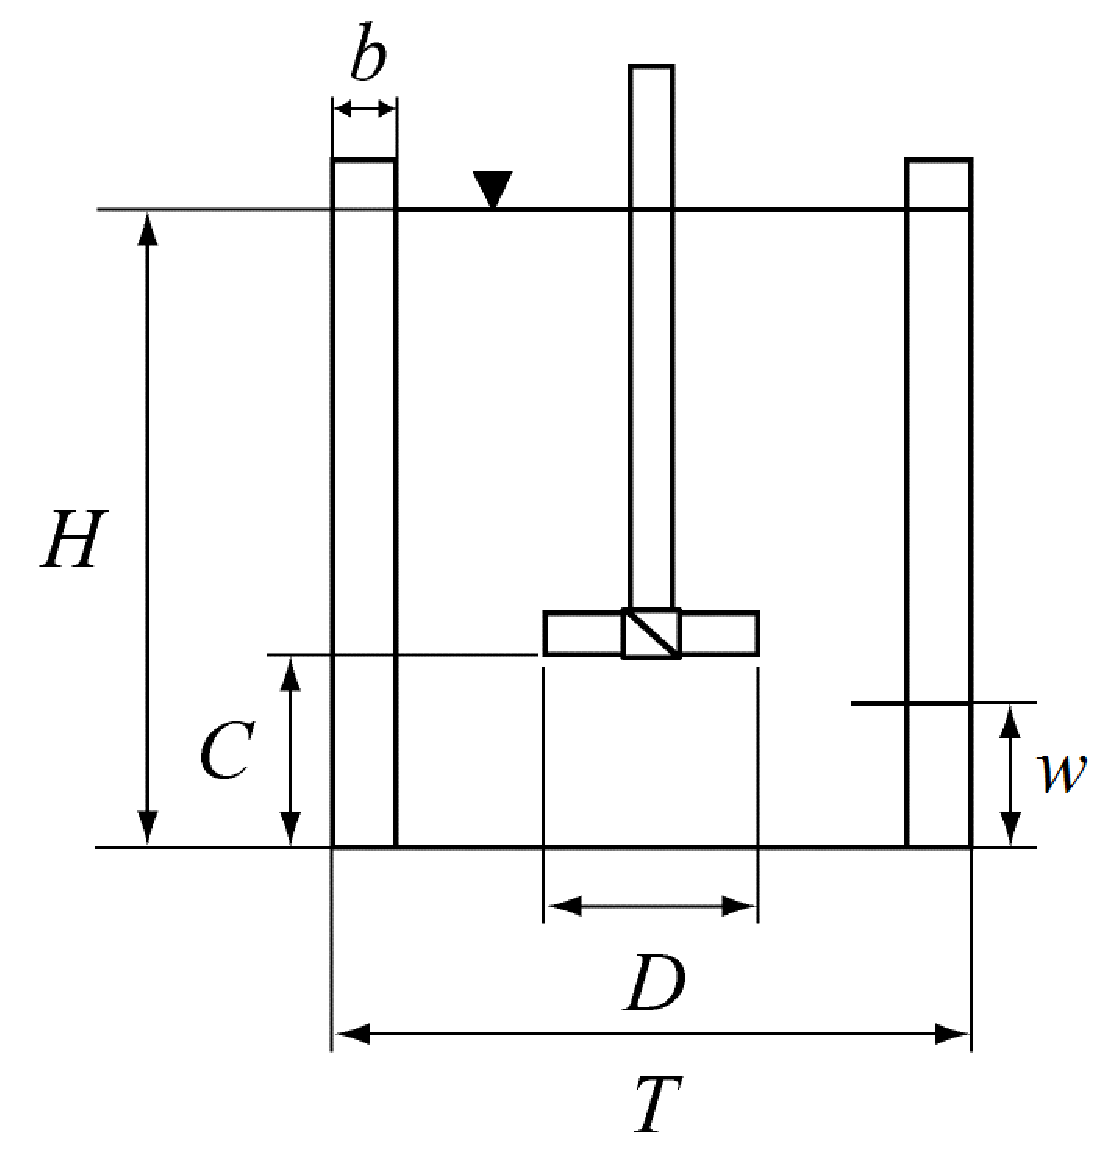
\includegraphics[scale=0.44]{images/mujedit.eps}
\caption{Geometrie experimentu}
\label{fig:nadoba}
\end{figure} 
Detailnější geometrie použitého míchadla je rozkreslena na obr. \ref{fig:imp}. Směr rotace hřídele byl volen tak, aby míchadlo vytvářelo proudění proti dnu nádoby. Frekvence jeho otáčení se pohybovala v~intervalu od \SI{3}{\per\second} do \SI{9}{\per\second}, což přibližně odpovídá Reynoldsovu číslu pro míchání ($Re_{M}$) od \num{24500} do \num{73800}.
\begin{figure}[t]
\centering
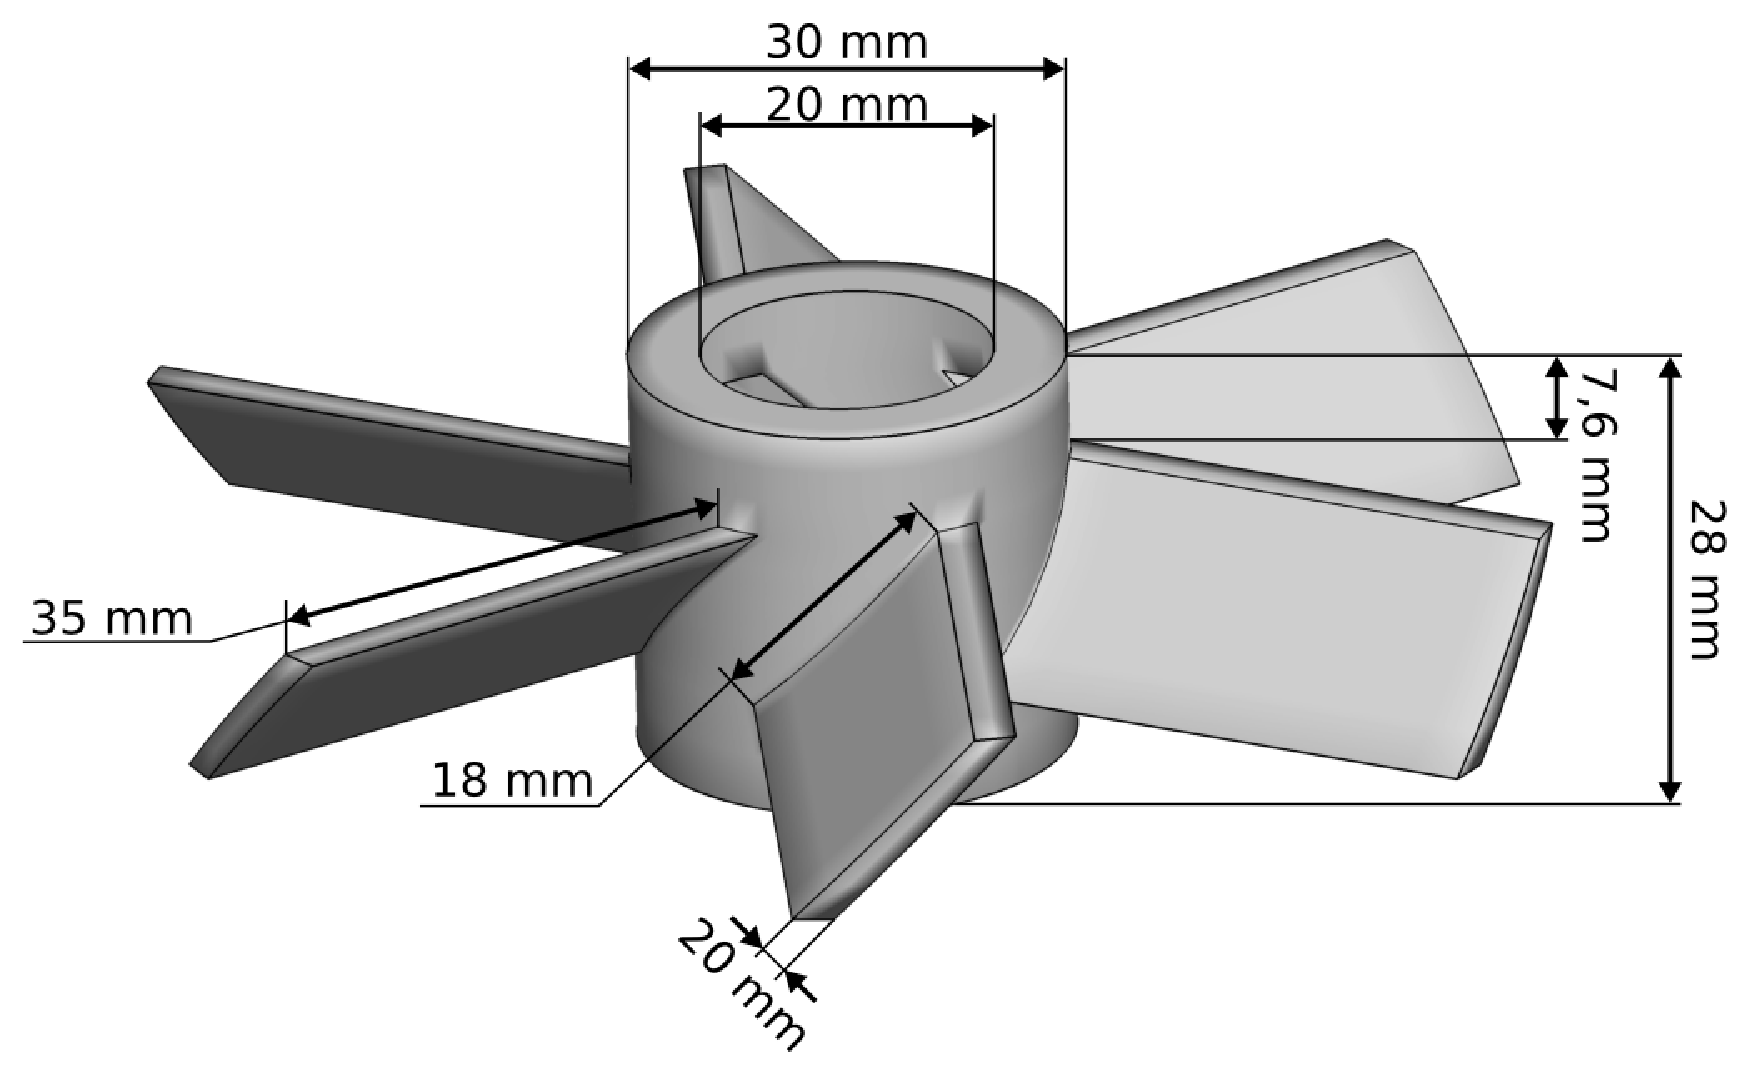
\includegraphics[scale=0.35]{images/imp.eps}
\caption{Geometrie míchadla}
\label{fig:imp}
\end{figure} 

Jako vsádka byla použita voda a polyvinylpyrrolidon (PVP), což je polymer rozpustný ve vodě s~newtonovských chováním. V~této práci byly využity dvě varianty této kapaliny \pvpP a \pvpS lišící se dynamickou viskozitou (\num{5} resp. \SI{7.5}{\milli\pascal\second}).  Pevnou fázi tvořily červené kuličky z~polyvinylchloridu (PVC) o~průměru \SI{1.02}{\milli\meter}. Vsádka postupně obsahovala 5, 10 a \volproc{15} těchto kuliček. Experimentálně stanovené vlastnosti kapalné a pevné fáze jsou shrnuty v~tab. \ref{tab:fyzvlast}. 
\begin{table}[h!]
\centering
\caption{Určené vlastnosti kapalné a pevné fáze}
\label{tab:fyzvlast}
\begin{tabular}{llrc}
\toprule
\textbf{Fáze} & \textbf{Veličina} & \textbf{Hodnota} &\textbf{Jednotka} \\
\midrule

voda \\
	& hustota & \num{999.50} & \si{\kilogram\per\cubic\meter} \\
	& dynamická viskozita & \num{1.138} & \si{\milli\pascal\second} \\
\pvpP \\
	& hustota & \num{1011.44} & \si{\kilogram\per\cubic\meter} \\
	& dynamická viskozita & \num{5.050} & \si{\milli\pascal\second} \\
\pvpS \\
	& hustota & \num{1024.18} & \si{\kilogram\per\cubic\meter} \\
	& dynamická viskozita & \num{7.615} & \si{\milli\pascal\second} \\
PVC \\
	& hustota & \num{1136.0} & \si{\kilogram\per\cubic\meter} \\
	& průměr & \num{1.02} & \si{\milli\meter} \\
	& mezerovitost & \num{0.384} & -- \\

\bottomrule
\end{tabular}
\end{table}

Pro stanovení průběhu homogenizace vsádky byla využita stopovací látka v~podobě chloridu sodného. Jeho roztok o~objemu přibližně \SI{5}{\milli\litre} byl nastříknut na volnou hladinu mezi narážku a hřídel míchadla. Koncentrace této látky byla měřena pomocí vodivostní sondy umístěné na opačné straně nádrže ve výšce $w = T/4$ ode dna. Výstupní analogový signál z~čidla o~vzorkovací frekvenci \SI{3}{\hertz} byl po zpracování A/D převodníkem uložen v~připojeném počítači k~dalšímu zpracování. Zaznamenané hodnoty napětí byly následně přepočítány na bezrozměrnou koncentraci $c^{*}(t)$ podle vzorce:    
\begin{equation}
	c(t)^{*} = \frac{c(t) - c_{0}}{c_{\infty} - c_{0}} \approx \frac{U(t) - U_{0}}{U_{\infty} - U_{0}}
	\label{eq:bezkonU}
\end{equation}
přičemž symbol $U$ značí hodnotu napětí ve zvoleném čase a význam ostatních symbolů je stejný jako ve vztahu \ref{eq:bezkon}. Doba po které dosáhla fluktuace bezrozměrné koncentrace hodnoty menší než \SI{5}{\percent}, byla považována za dobu homogenizace ($t_{mix}$). 

Během experimentu byly také pořizovaly digitální fotografie míchaného systému lišící se koncentrací pevné fáze, použitou kapalnou vsádkou a rychlostí otáčení míchadla. Získané fotografie byly poté použity k~orientačnímu stanovení výšky vznosu pevné fáze. 

	\chapter{Výpočetní část}

\section{Tvorba geometrie a výpočetní sítě}

Prvním krokem před každou CFD simulací je tvorba geometrie systému a její následná diskretizace (tzv. vysíťování). Výpočetní doména byla vytvořena podle geometrie experimentu uvedené v~kapitole \ref{chap:exp} prostřednictvím programu ANSYS DesignModeler 12.1. Pro snížení výpočetní náročnosti byla simulována pouze část nádrže obsahující kapalinu bez přítomnosti vzduchu. Míchací nádoba byla rozdělena na část rotační, kterou tvořil válec o~výšce \SI{5.2}{\centi\meter} a průměru \SI{16.5}{\centi\meter}. Zmíněná rotační doména obsahující míchadlo a část hřídele začínala ve vzdálenosti \SI{1.35}{\centi\meter} od spodní hrany míchadla. Zbývající část systému obsahující větší část hřídele, dno, stěny a narážky nádoby představovala stacionární oblast. Vytvořená geometrie systému je zachycena na obrázku \ref{fig:geo}, kde zelenou barvou je znázorněna rotační zóna kolem míchadla. 

\begin{figure}[h!]
\centering
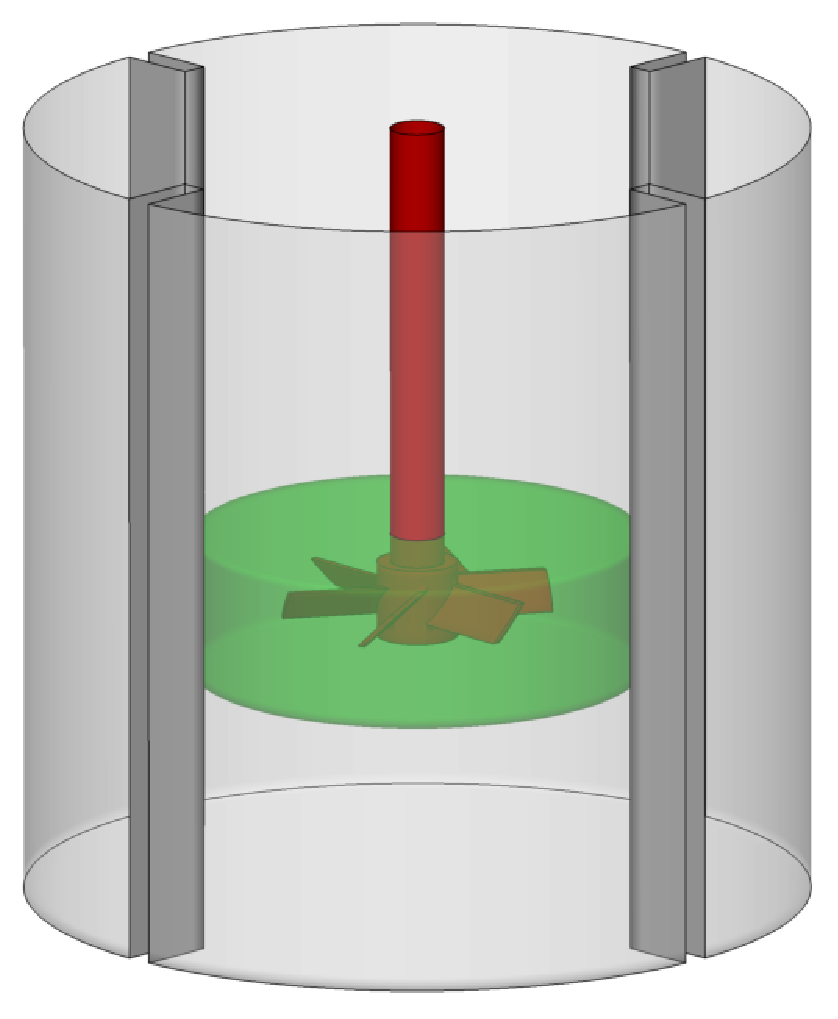
\includegraphics[scale=0.5]{images/geo.eps}
\caption{Geometrie systému}
\label{fig:geo}
\end{figure} 

Pro tvorbu výpočetní sítě byl využit program ANSYS Meshing 12.1, do kterého byla načtena geometrie nádoby vytvořená v~předcházejícím kroku. Výsledná nestrukturovanou síť se skládala z~\num{264398} buněk o~průměrném objemu \SI{0.07}{\milli\litre}. Jednalo se převážně o~šestistěnné buňky, přičemž pouze v~oblasti pod míchadlem se vyskytovalo \num{132} třístěnných hranolů. Řez diskretizovanou doménou je zachycen na obrázku \ref{fig:mesh}, ze kterého si lze povšimnout, že v~oblasti míchadla je síť úmyslně zahuštěna. 
\begin{figure}[t]
\centering
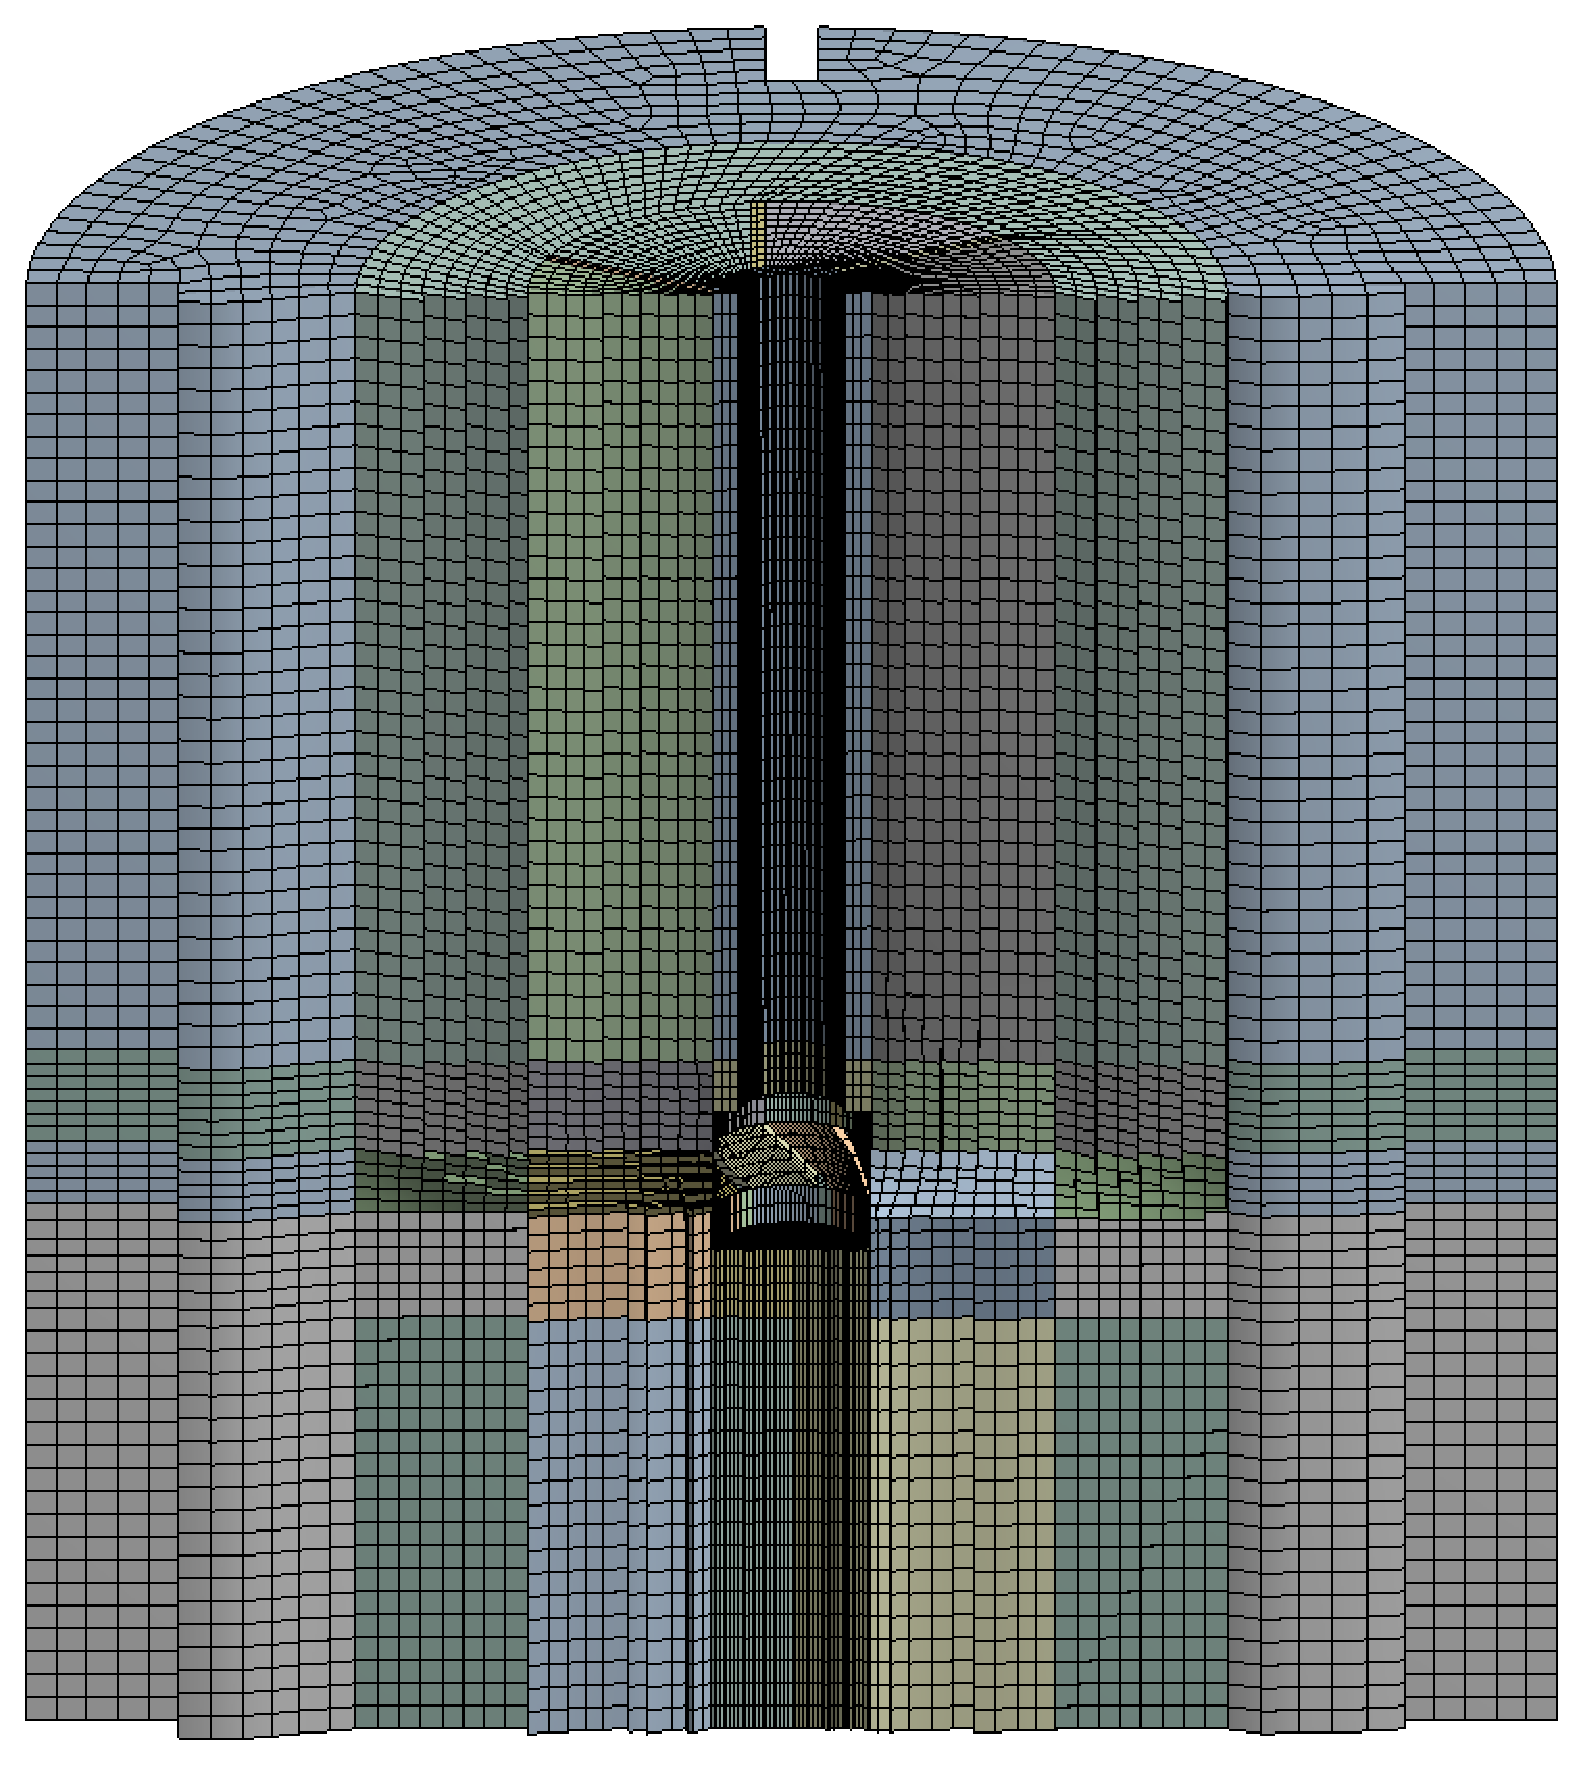
\includegraphics[scale=0.28]{images/mesh.eps}
\caption{Řez výpočetní sítí}
\label{fig:mesh}
\end{figure} 
Pro posouzení kvality vytvořené sítě existuje celá řada kritérií, avšak mezi jedno z~nejpoužívanější patří tzv. šikmost (angl. skewness) definovaná jako:
\begin{equation}
      skewness = \mathsf{max}\kula{\frac{\beta_{max} - \beta_{e}}{180 - \beta_{e}}, \frac{\beta_{e} - \beta_{min}}{\beta_{e}}}
  	\label{eq:skw}
\end{equation} 
kde $\beta_{min}$, $\beta_{max}$ značí nejmenší resp. největší úhel v~buňce a $\beta_{e}$ představuje úhel v~pravidelném (ideálním) elementu. Šikmost se obecně pohybuje v~intervalu od \num{0} do \num{1}, přičemž nulová hodnota značí nejlepší kvalitu buňky, a naopak šikmost rovna jedné indikuje úplnou degeneraci elementu. Vybrané charakteristiky této veličiny pro vytvořenou výpočetní doménu jsou uvedeny v~tabulce \ref{tab:skw_tab}. Z~uvedených hodnoty vyplývá, že vygenerovaná síť dosahuje výborné kvality.
\begin{table}[h!]
\centering
\caption{Charakteristiky šikmosti pro vytvořenou síť}
\label{tab:skw_tab}
\begin{tabular}{lr}
\toprule
\textbf{Charakteristika} & \textbf{Hodnota} \\
\midrule

Maximální šikmost & \num{0.666} \\
Průměrná šikmost & \num{0.164} \\
Směrodatná odchylka šikmosti & \num{0.123} \\

\bottomrule
\end{tabular}
\end{table}

\section{Uživatelem definované funkce}
Uživatelem definované funkce (UDF) jsou moduly načítané do softwaru \flu, jenž rozšiřují nebo upravují schopnosti řešiče. Například se může jednat o~vytvoření vlastních počátečních a okrajových podmínek, změnu materiálových vlastností a modifikaci simulačních modelů. Pro tvorbu zdrojových souborů se využívá programovací jazyk C. Vytvořené soubory jsou následně zkompilované do dynamické knihovny.

Právě pomocí uživatelem definovaných funkcí byly implementovány modely pro koeficient odporu uvedené v~tabulce \ref{tab:cds} spolu s~klasickým modelem dle Schillera a Neumanna (vztah \ref{eq:schlneu}). Navíc kromě korelací pro výpočet součinitele odporu byla do této knihovny naprogramována funkce pro výpočet kvality suspenze podle vztahu (\ref{eq:kvasus}). Všechny vytvořené zdrojové kódy jsou uvedeny v~kapitole \nameref{sec:priloha}.

\section{Vlastní CFD simulace}
Ke studiu suspendace pomocí CFD simulaci byl využit komerční software \flu{} 12.1.4, do kterého byla načtena vytvořená výpočetní síť. Následně byly nastaveny okrajové podmínky pro jednotlivé části řešené domény. Pro všechny fyzické části nádrže (dno, stěny, narážky, hřídel a míchadlo) byla vybrána okrajová podmínka typu stěna, pro kterou platí, že rychlost proudění na jejím povrchu je nulová. Z~důvodu jednoduchosti byla pro hladinu kapaliny zvolena okrajová podmínka symetrie, jenž vyjadřuje nulovou hodnotu gradientu pro jednotlivé veličiny. Tato volba je obvyklá pro systémy, kde je pozornost věnována dějům probíhající uvnitř nádoby a nikoliv na mezifázovém rozhraní, což je právě případ suspendace. Pohyb rotační části domény byl v~případě stacionární simulace modelován pomocí metody vícenásobných souřadnicových soustav (MRF) a pro nestacionární (dynamickou) simulaci byla použita technika klouzající sítě (SM). 

Proudění v~nádobě bylo považováno za izotermní, nestlačitelné a plně turbulentní. Pro popis turbulence byl využit standardní \keps{} turbulentní model s~disperzní modifikací pro vícefázový systém. Navíc během simulace byl zohledněn efekt turbulentní disperze dle doporučení autorů \citet{lju01} nebo \citet{tamb09}. Z~mezifázových sil byla modelována pouze odporová síla jakožto dominantní člen. Pro popis koeficientu odporu byly využity korelace dodané v~podobě UDF knihovny. V~provedených simulacích byla největší pozornost věnována modelu dle Khopkara, který byl navržen speciálně pro CFD simulaci suspendace v~míchaných nádobách.

Pro popis vícefázového proudění v~nádrží byl použit 
matematický model Eulerian-Eulerian, přičemž jako primární fáze 
byla zvolena voda nebo PVP a sekundární fázi tvořily kuličky z~PVC. 
Při použití této techniky se pevná fáze modeluje jako ideální 
kapalina (bez vnitřního tření). Zmíněnou skutečnost bylo třeba 
zohlednit během nastavení simulace. Viskozita pevné fáze byla proto zvolena téměř nulová ($\SI{e-10}{\pascal\second}$) a jednotlivé složky tečného napětí na všech stěnách byly rovněž nastaveny na nulu. Pro porovnání byly některé výpočty provedeny s~vícefázovým přístupem Eulerian-Granular. Hodnota viskozity zrnité fáze byla určena pomocí vztahů navržených \citet{syam93}. Členy jako radiální distribuční funkce, tlak pevné fáze a dilatační viskozita byly stanoveny pomocí modelů, jenž navrhli autoři \citet{lun84}.  

Vlastní CFD výpočet byl proveden jako nestacionární, aby bylo možné sledovat průběh suspendace a dynamiku vzniku suspenzního mraku. Na začátku každé simulace byla na dno nádoby umístěná pevná fáze o~zvolené koncentraci 5, 10 nebo \volproc{15}. Pro potřeby počáteční podmínky bylo zvolené nulové rychlostní pole spolu s~hodnotou turbulentní kinetické energie rovné \SI{e-3}{\meter\squared\per\second\squared} a její rychlosti disipace \SI{e-3}{\meter\squared\per\second\cubed}. K~určení rychlostního a tlakového pole byla využita vícefázová modifikace algoritmu SIMPLE. Velikost časového kroku byla zvolena \SI{0.001}{\second}, přičemž v~každém kroku bylo provedeno maximálně \num{55} iterací. Konvergenční kritérium bylo splněno pokud hodnoty reziduí všech řešených veličin byly menší než \num{e-3}. Pro sledování konvergence výpočtu byla také monitorována síla působící na narážky nádoby a průměrná hodnota koeficientu odporu v~celém systému. V~prvních \num{100} časových krocích byly použity diskretizační náhrady pouze prvního řádu a podrelaxační faktory pro tlak, hybnost a turbulentní viskozitu byly sníženy na hodnotu \num{0.2}, \num{0.2} respektive \num{0.8}. Po této době následovalo přepnutí na diskretizační náhrady druhého řádu a nastavení všech podrelaxčních faktorů na své výchozí hodnoty. Celková doba simulace činila \SI{7}{\second}, což se dle experimentů jevila jako dostatečná doba k~ustálení tokového pole. Simulace probíhaly na počítači HP Z600 osazený dvěma procesory Intel Xeon X5570 a pamětí 24~GB s~operačním systémem CentOS 5.3 x86-64. Doba výpočtu jedné reálné vteřiny trvala přibližně 4 hodiny.

Získaná rychlostí pole byla poté využita ke stanovení doby homogenizace. Stopovací látka s~fyzikálními vlastnostmi stejnými jako kapalná fáze byla na počátku simulace umístěna \SI{2}{\centi\meter} po hladinu vsádky. V~průběhu výpočtu byly následně zaznamenávány hodnoty objemového zlomku indikační látky v~místě umístění vodivostní sondy.



  \chapter{Výsledky a diskuze}
Následující kapitola shrnuje výsledky provedených CFD simulací suspendace v mechanicky míchané nádobě. Navíc kde to situace umožňovala byly získaná data porovnány s dostupným experimentálním měřením.

\section{Rychlostní pole v nádobě}
Pro porovnání vlivu zvoleného turbulentního modelu na výsledné rychlostní pole bylo provedeno několik stacionárních simulací míchaní vodné vsádky. 

Na obr. \ref{fig:velfield} jsou znázorněno vektorové pole rychlosti kapaliny v~řezu nádobou pro jednotlivé turbulentní modely a frekvenci otáčení míchadla \SI{7}{\per\second}. Ze všech obrázků je dobře patrný vznik primární cirkulační smyčky která je charakteristická pro axiální míchadla. Navíc si lze také povšimnout tvorby sekundárních cirkulačních smyček v~prostoru pod míchadlem. Tento jev byl například experimentálně pozorován autory \citet{hos10} při zvolené světlé výšce míchadla od $C=T/2$ do $C=T/6$. Důležitý je také fakt, že i při srovnání s výpočetně náročnějším Reynoldsovým napěťovým modelem (obr. \ref{fig:RMS}) se jednotlivá rychlostní pole od sebe významně neliší.

\begin{figure}[h!]
 \centering

  \subfloat[Standardní \keps{}]{\label{fig:std}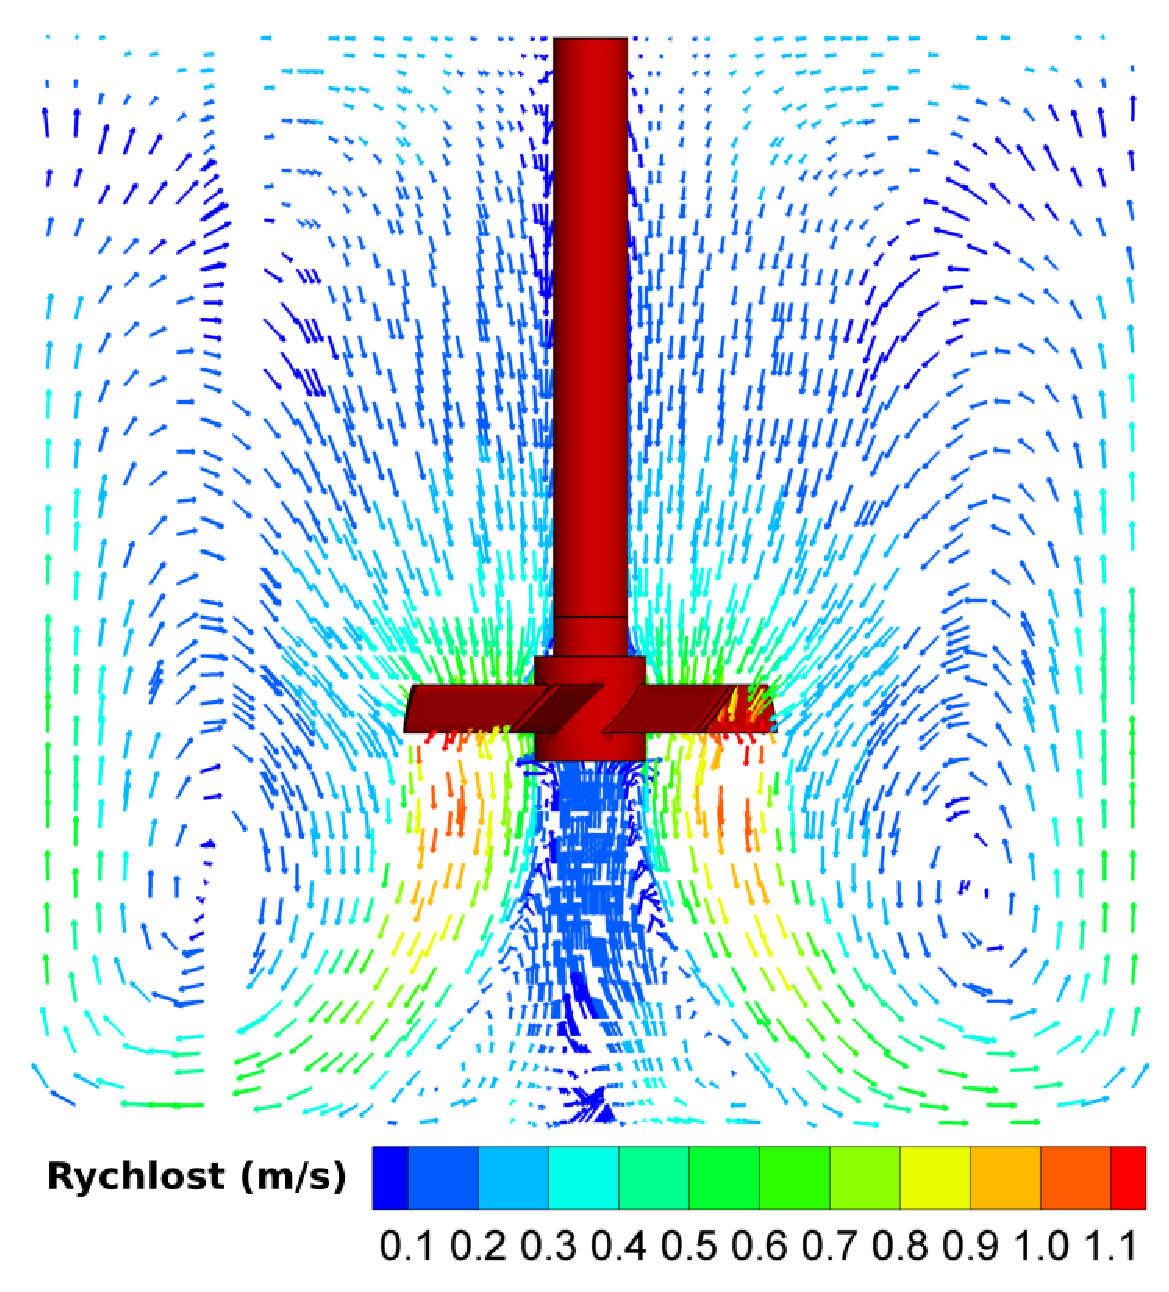
\includegraphics[scale=0.38]{Results/Velocity/keps-std.eps}}  
  \qquad 
  \subfloat[RNG \keps{}]{\label{fig:rng}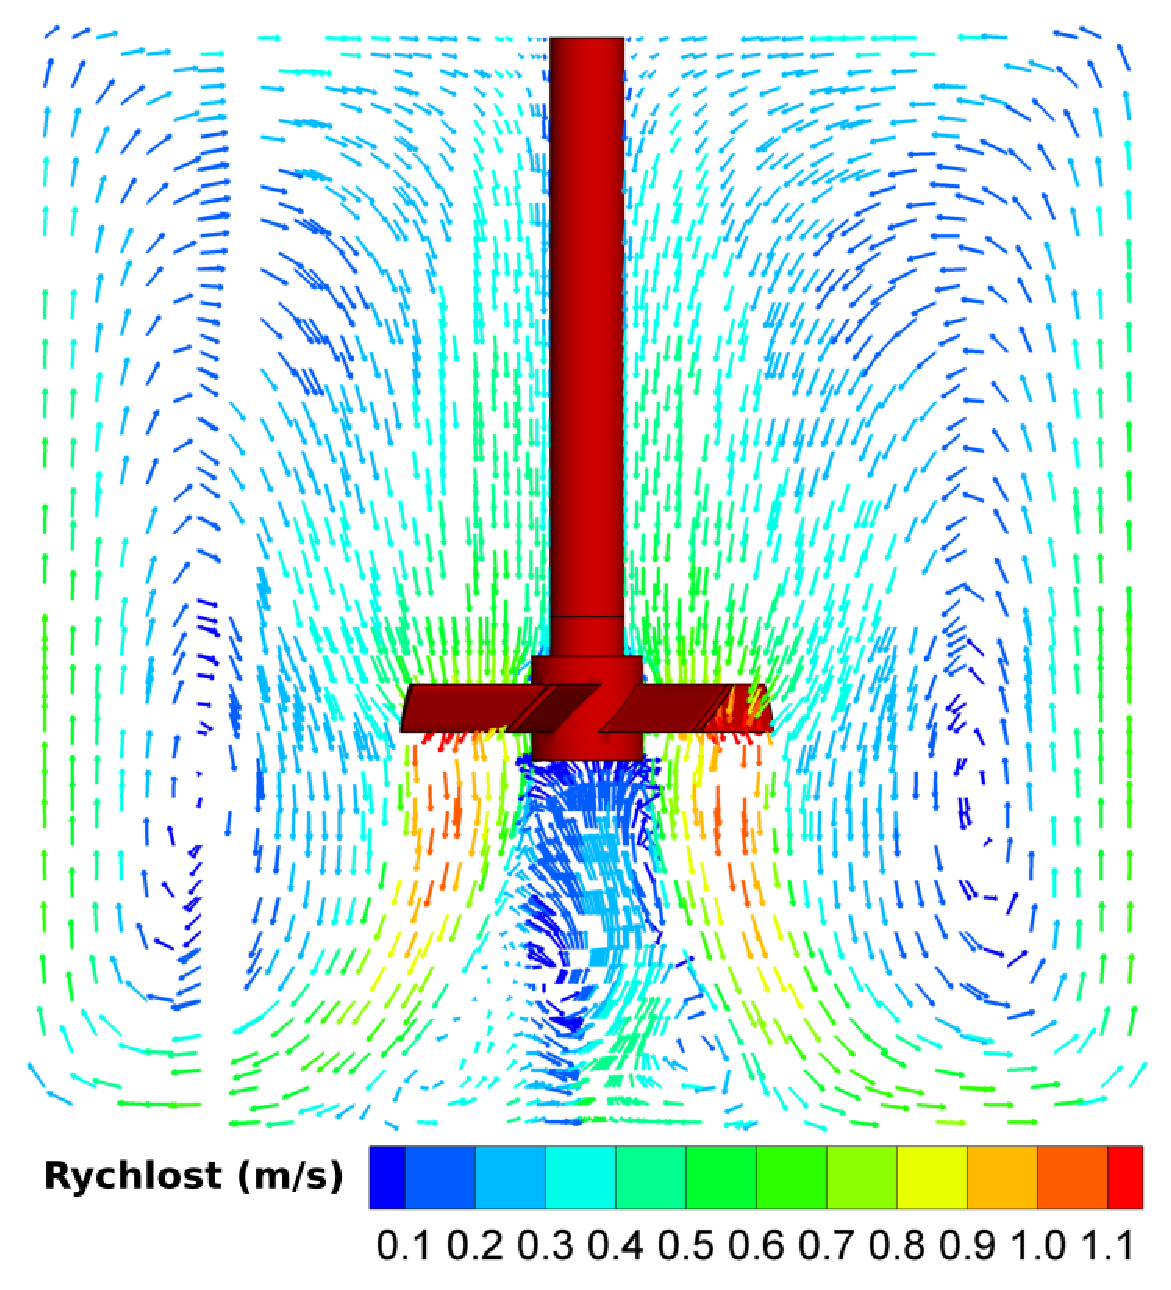
\includegraphics[scale=0.38]{Results/Velocity/keps-RNG.eps}}
\end{figure}
\newpage
\begin{figure}[t!]
  \addtocounter{subfigure}{2}
 \centering
  \subfloat[Realisable \keps{} ]{\label{fig:real}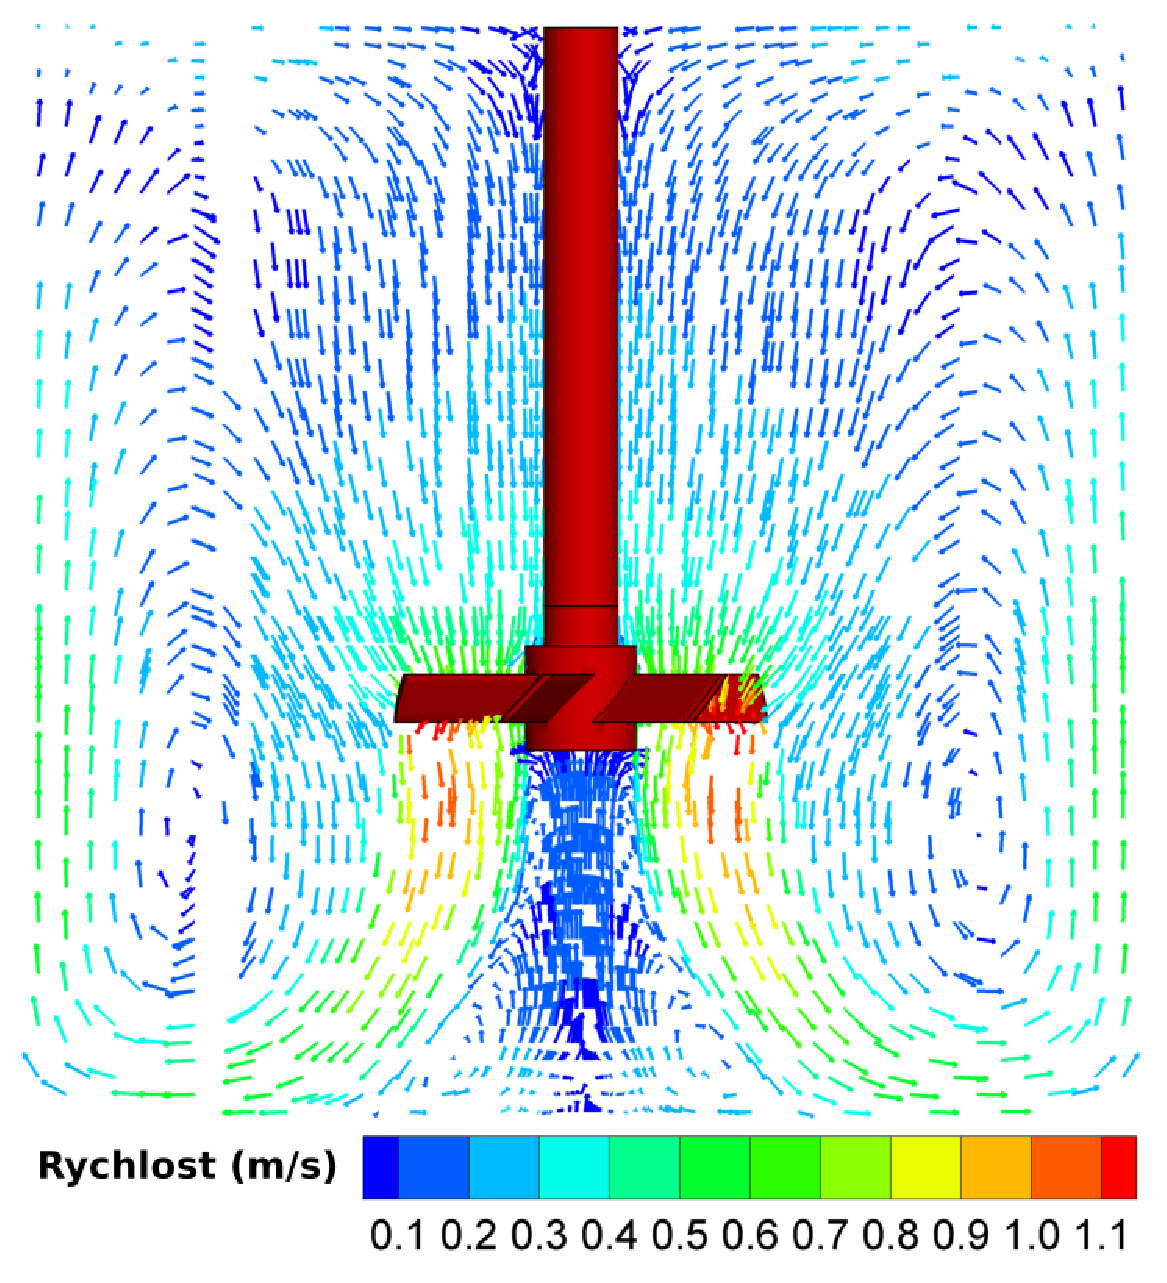
\includegraphics[scale=0.38]{Results/Velocity/keps-real.eps}}
  \qquad
  \subfloat[Standardní RMS]{\label{fig:RMS}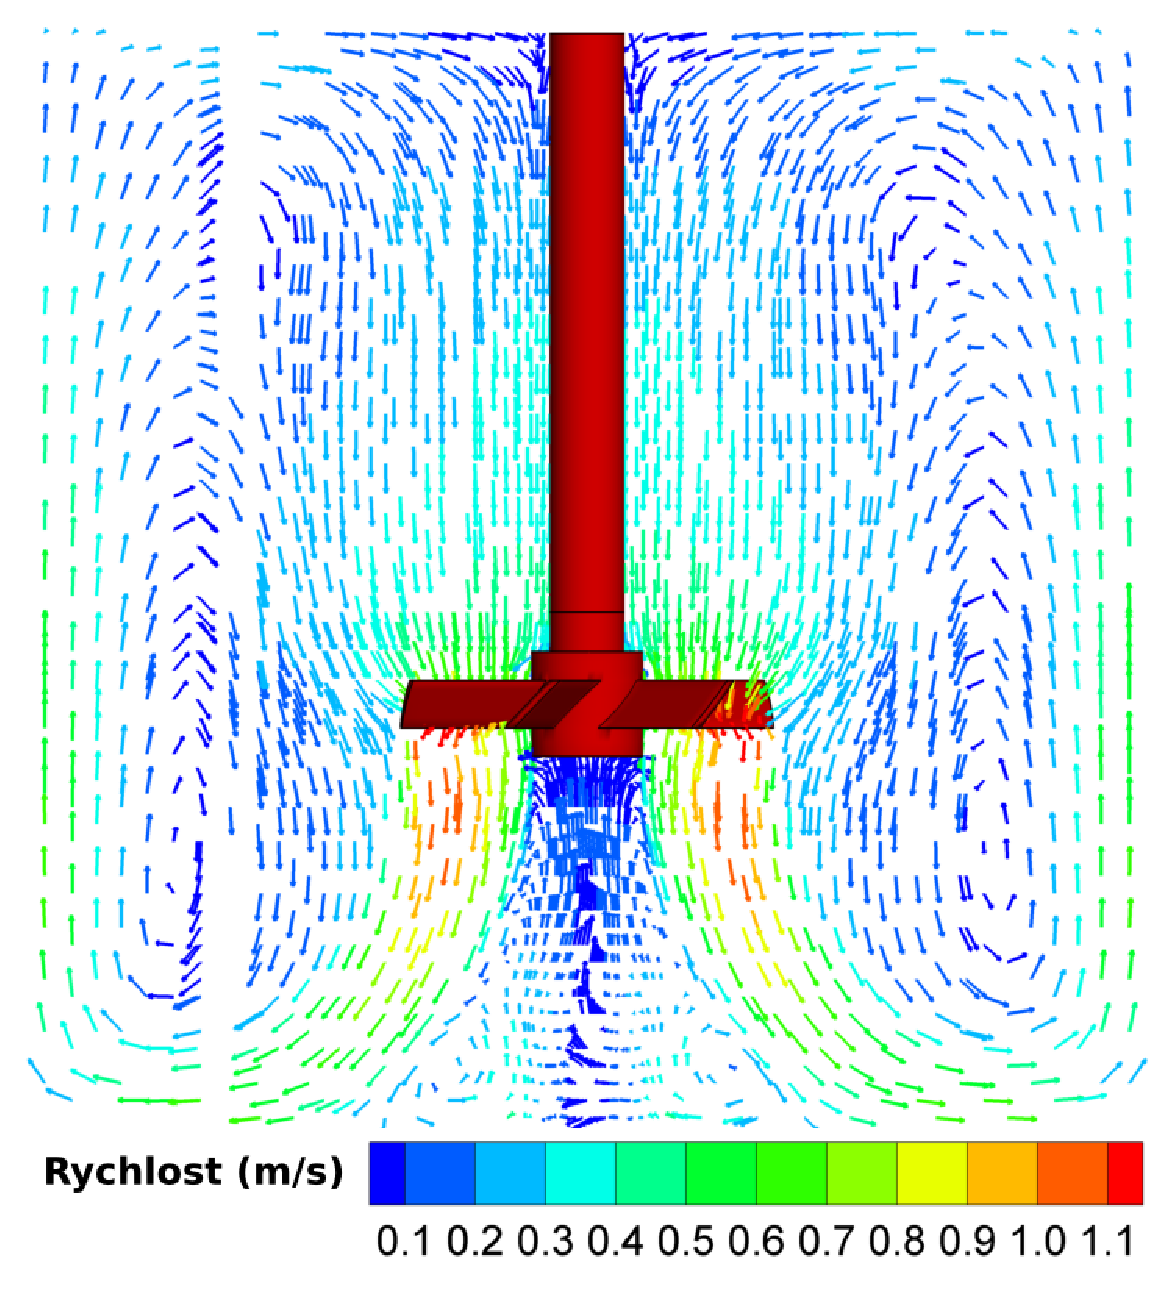
\includegraphics[scale=0.38]{Results/Velocity/RMS.eps}}
  \caption{Vektorové pole rychlosti pro různé turbulentní modely}
  \label{fig:velfield}
\end{figure}

Graf \ref{grf:velfield} zachycuje závislost mezi celkovou rychlostí pohybu kapaliny a vzdáleností ode dna nádoby ($y$) pro jednotlivé turbulentní modely. Konkretní hodnoty pro tento byly získány ve vzdálenosti \SI{0.5}{\centi\meter} podél jedné z narážek nádoby. Z grafu je dobře patrné, že u dna nádrže dochází nárůstu rychlosti tekutiny vlivem působení primární cirkulační smyčky.

\begin{grf}[h!]
 \centering
  \includegraphics[scale=0.45]{Results/Velocity/velField.eps}
  \caption{Průběh velikosti rychlosti tekutiny v nádobě}
  \label{grf:velfield}
\end{grf}

\section{Srovnání modelů pro koeficient odporu}
Jednotlivé modely pro koeficient odporu uvedené v podkapitole \ref{kap:cd} byly porovnány během nestacionární simulace systému obsahující jako vsádku \volproc{5} kuliček z PVC a kapalinu \pvpP. Rychlost otáčení míchadla byla v tomto případě opět nastavena na \SI{7}{\per\second}.

Obr. \ref{fig:cd2} zobrazuje kontury objemového zlomku pevné fáze v~řezu míchací nádobou pro vybrané korelace koeficientu odporu. Tyto údaje byly získány v~času simulace \SI{2}{\second}. 
\begin{figure}[h!]
 \centering

  \subfloat[Schiller-Naumann]{\label{fig:neu2}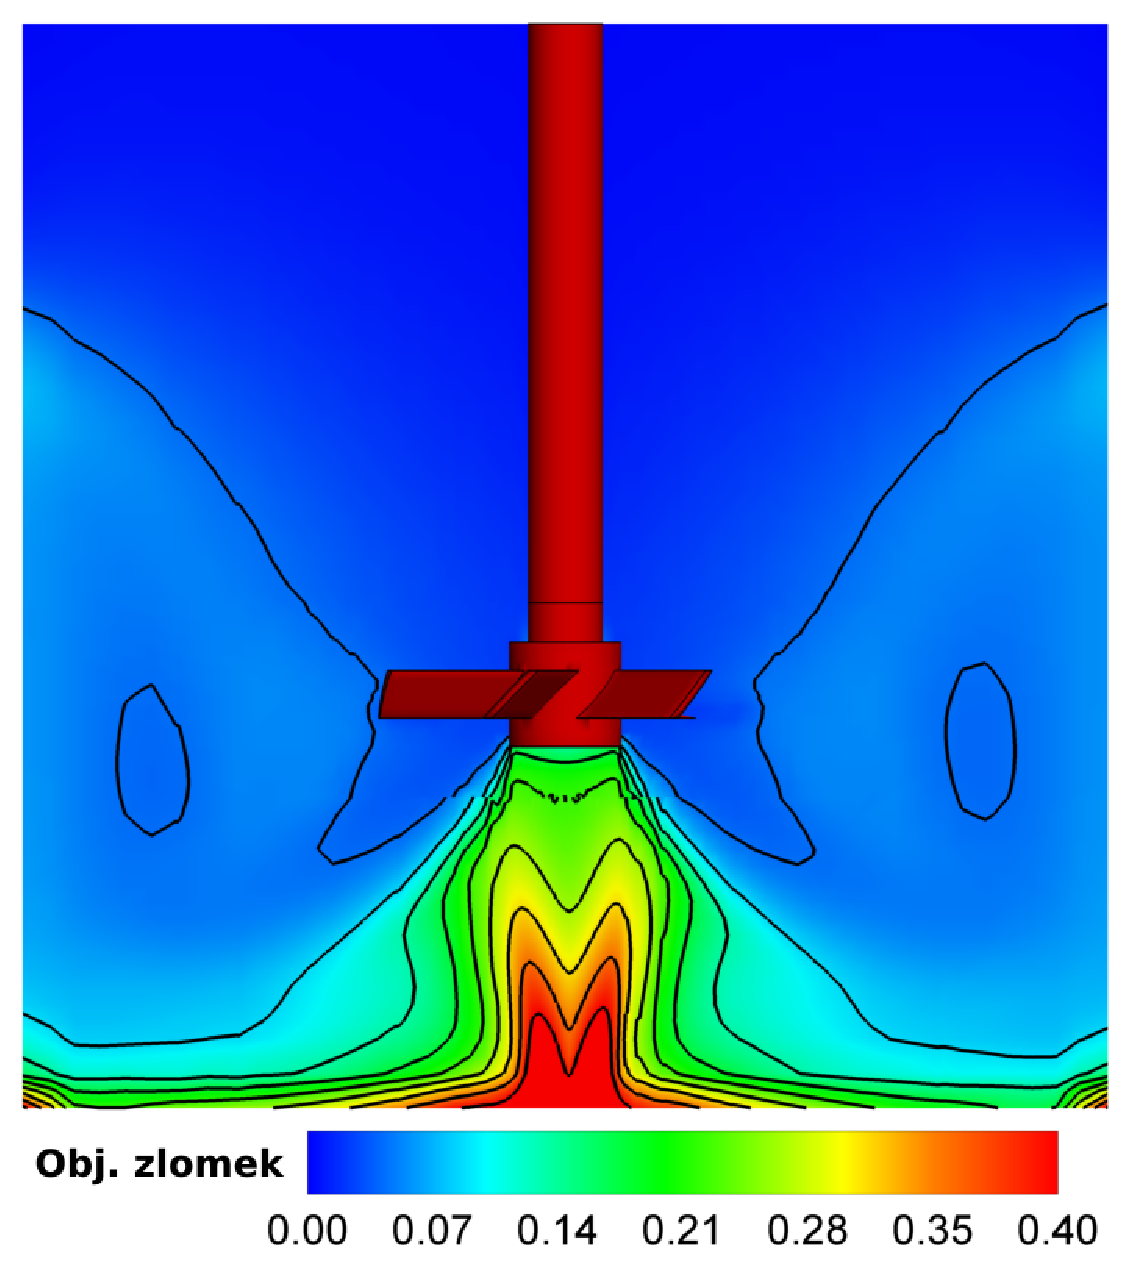
\includegraphics[scale=0.38]{Results/CDComp/neu-2s.eps}}  
  \qquad             
  \subfloat[{Brucato}]{\label{fig:bru2}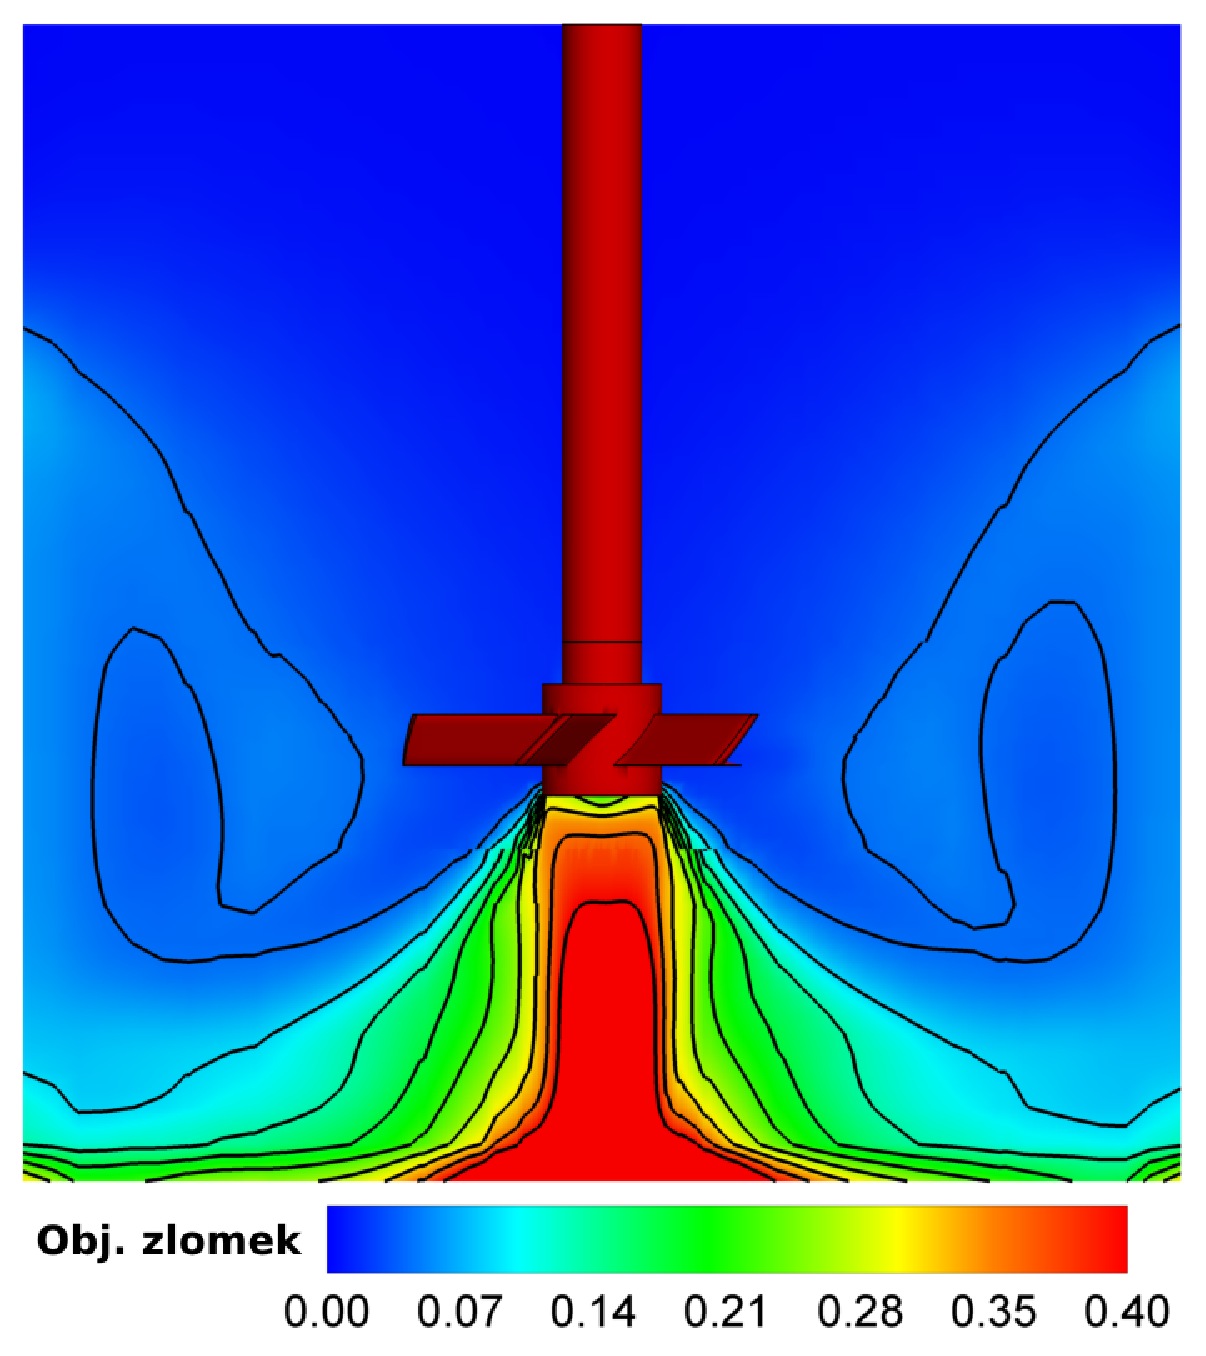
\includegraphics[scale=0.357]{Results/CDComp/bru-2s.eps}}
%\end{figure}
%\newpage
%\begin{figure}[t!]
	%\centering{}
  %\addtocounter{subfigure}{2}
  \\
  \subfloat[{Pinelli}]{\label{fig:pin2}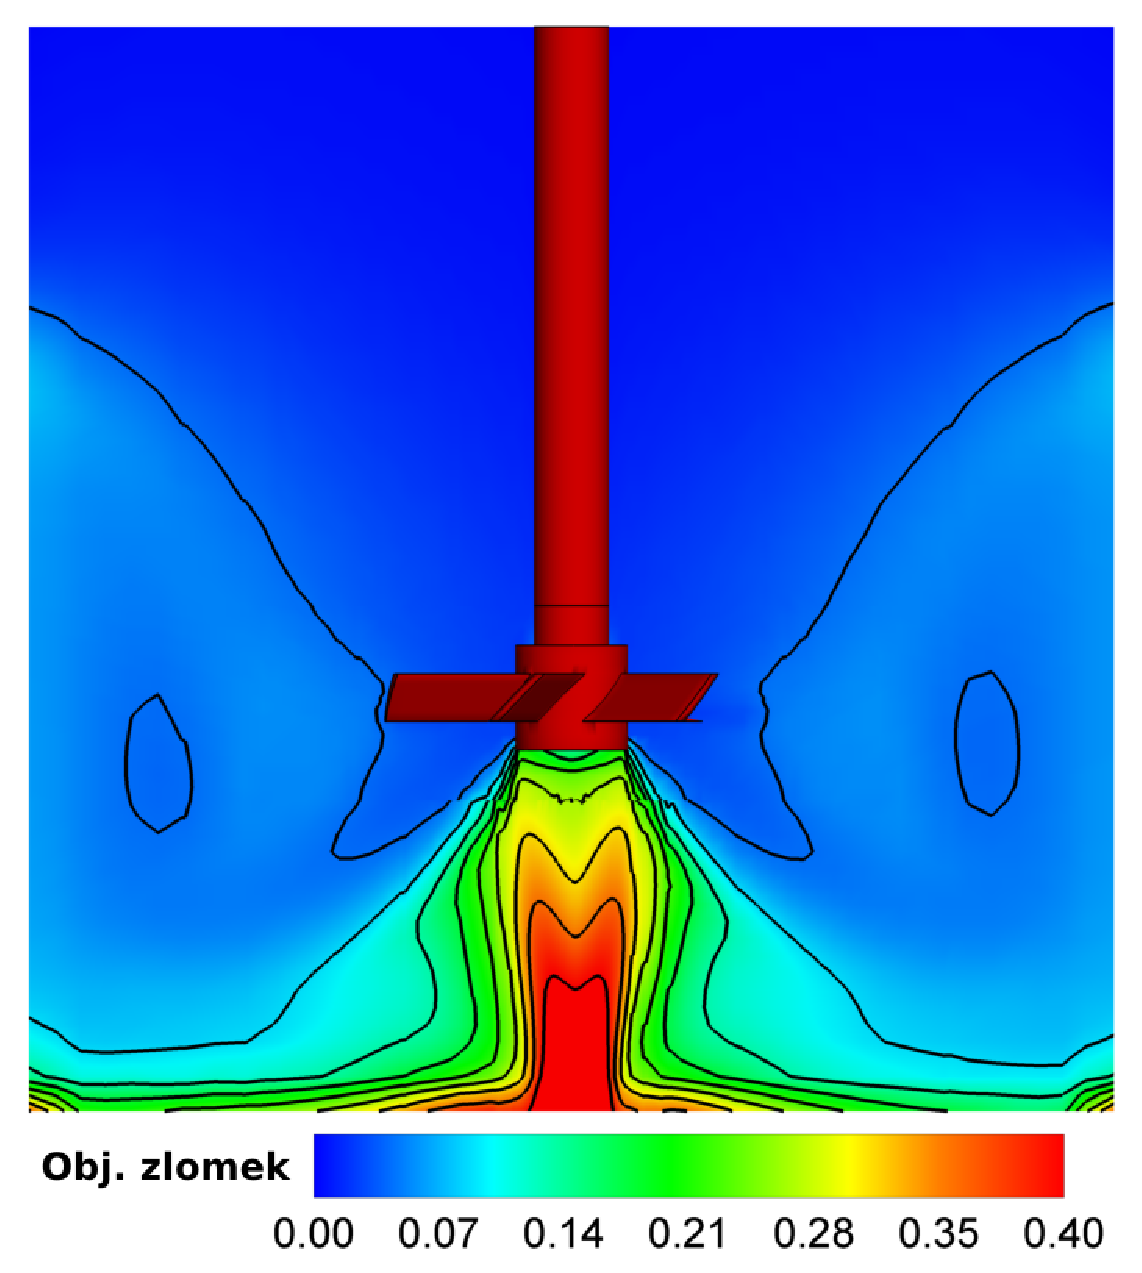
\includegraphics[scale=0.38]{Results/CDComp/pin-2s.eps}}
  \qquad
  \subfloat[{Khopkar}]{\label{fig:kho2}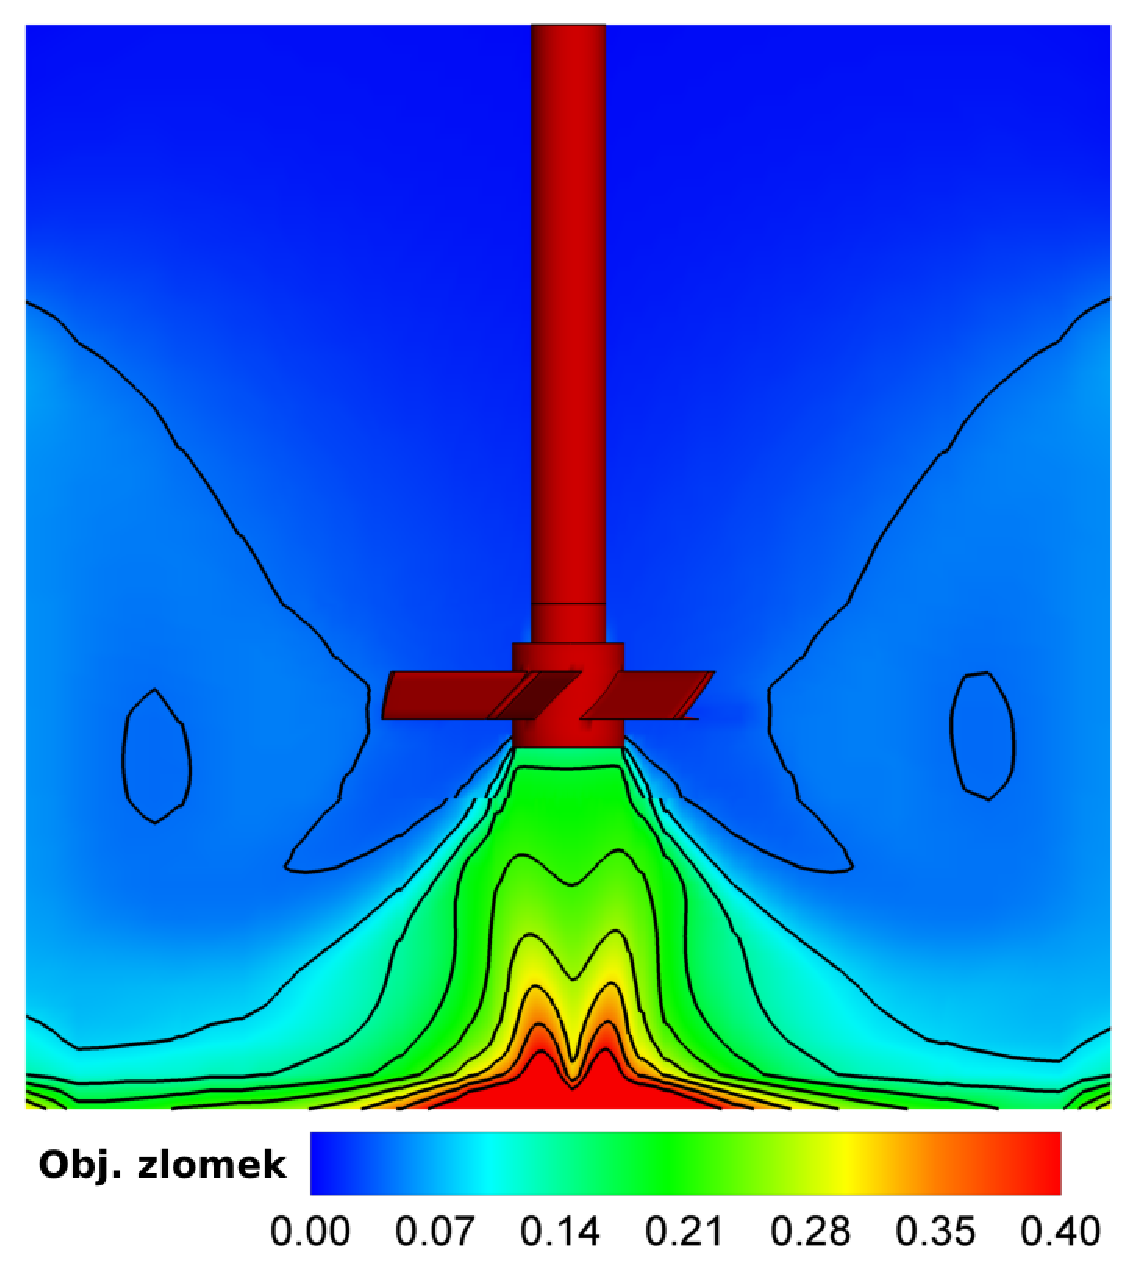
\includegraphics[scale=0.38]{Results/CDComp/kho-2s.eps}}
  \caption{Objemový zlomek pevné fáze v~čase \SI{2}{\second}}
  \label{fig:cd2}
\end{figure}
\newpage
\noindent Z~obrázků je dobře patrné, že přímo pod míchadlem je největší koncentrace pevné fáze vlivem sekundárních cirkulačních smyček, což se podařilo pozorovat i během experimentálního měření.

Série obrázků \ref{fig:cd7} zachycuje objemový zlomek pevné fáze v~řezu nádobou, avšak v čase simulace \SI{7}{\second}. Částice z PVC jsou již značně rozptýleny, ale stále se pod míchadlem nachází oblasti s jejich zvýšenou koncentrací. Nicméně v celé nádobě jsou rozdíly v distribuci pevné fáze mezi jednotlivými modely pro koeficient odporu poměrně zanedbatelné.

\begin{figure}[h!]
 \centering
  \subfloat[Schiller-Naumann]{\label{fig:neu7}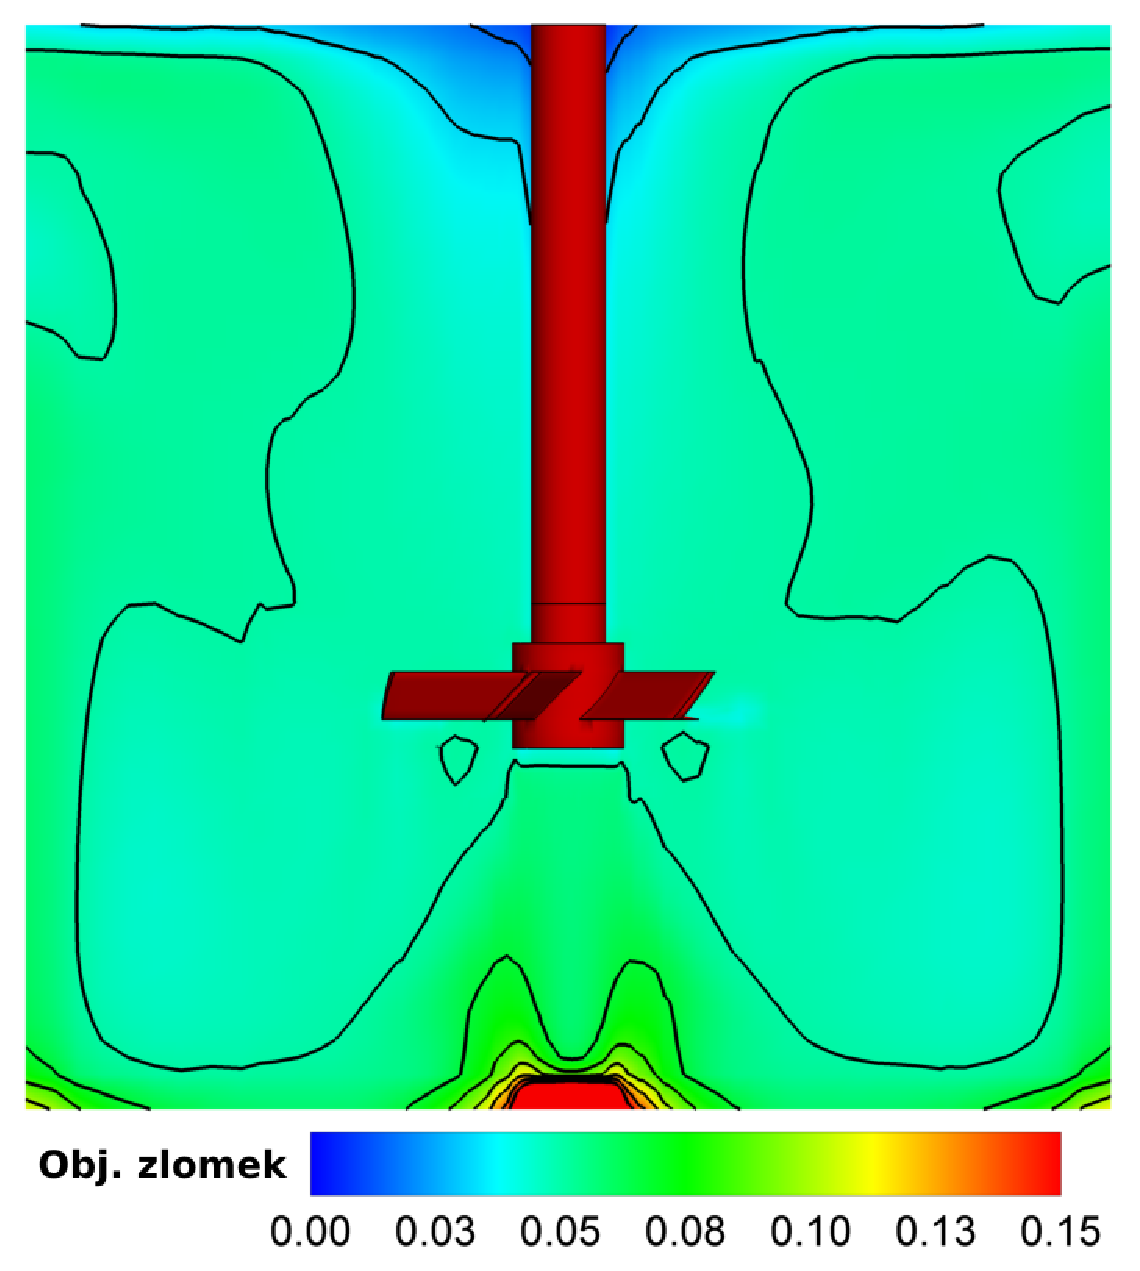
\includegraphics[scale=0.38]{Results/CDComp/neu-7s.eps}}  
  \qquad             
  \subfloat[{Brucato}]{\label{fig:bru7}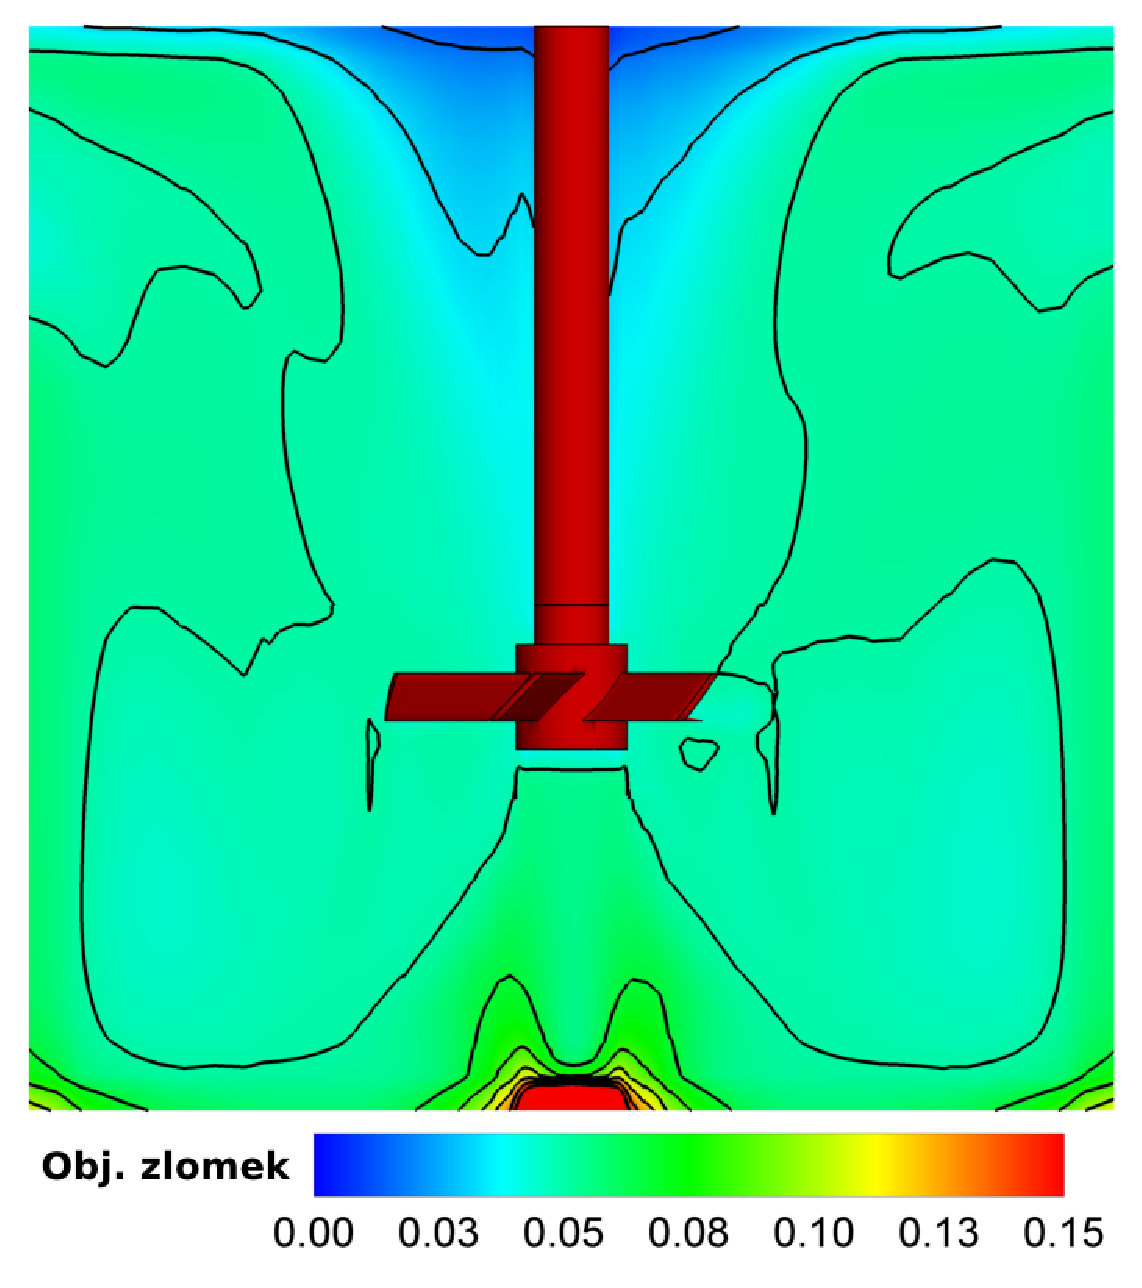
\includegraphics[scale=0.38]{Results/CDComp/bru-7s.eps}}
%\end{figure}
%\newpage
%\begin{figure}[t!]
	 %\centering{}
	 \\
  \subfloat[{Pinelli}]{\label{fig:pin7}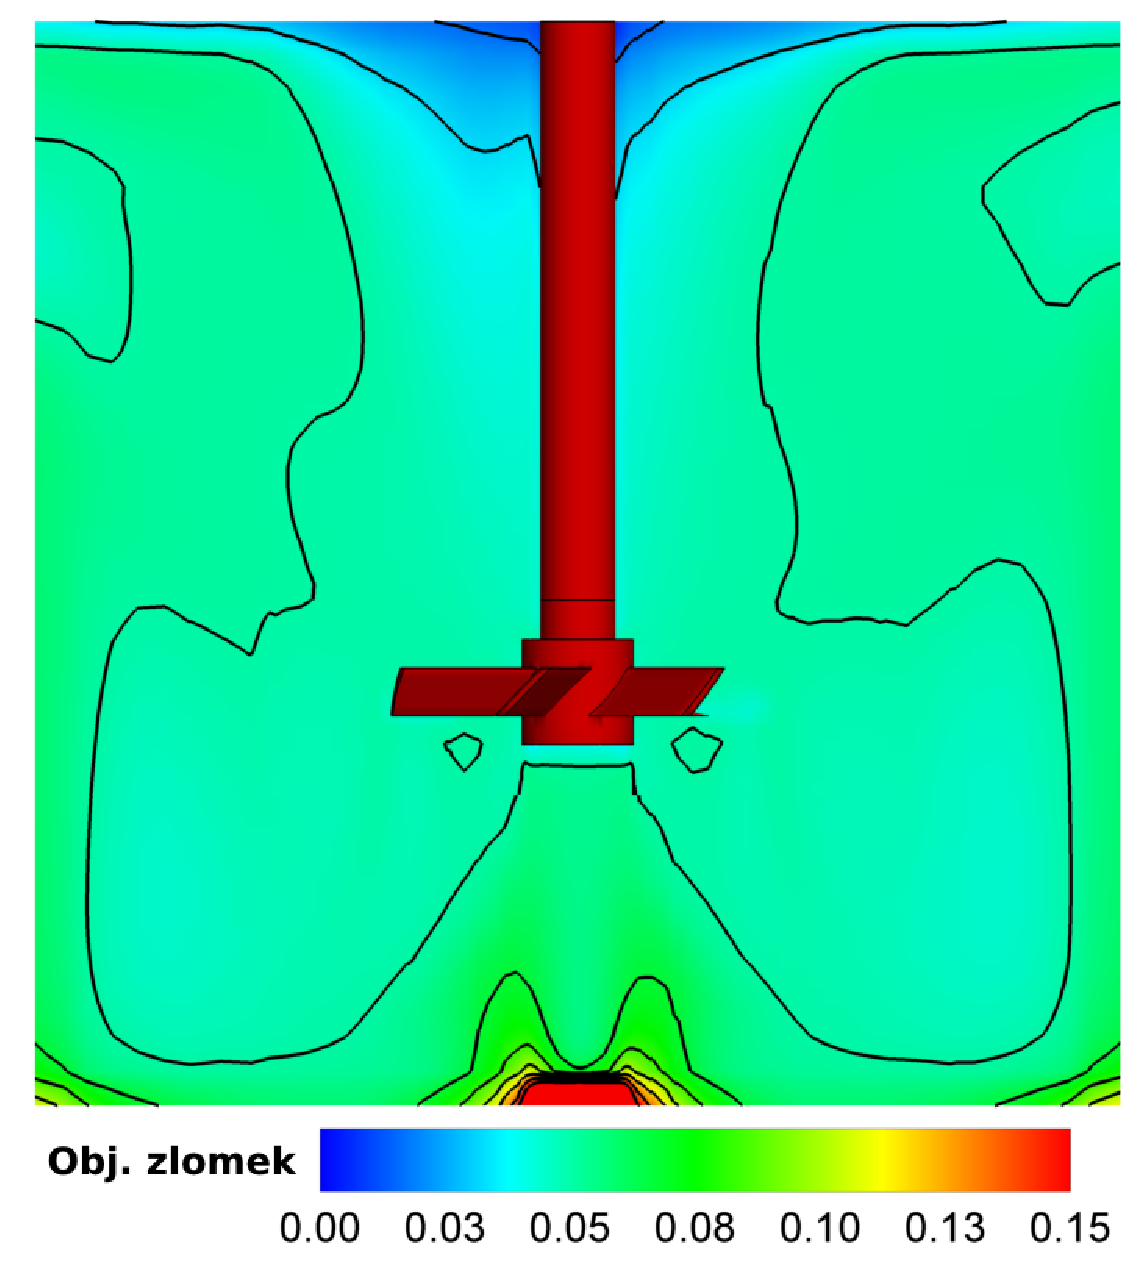
\includegraphics[scale=0.38]{Results/CDComp/pin-7s.eps}}
  \qquad
  \subfloat[{Khopkar}]{\label{fig:kho7}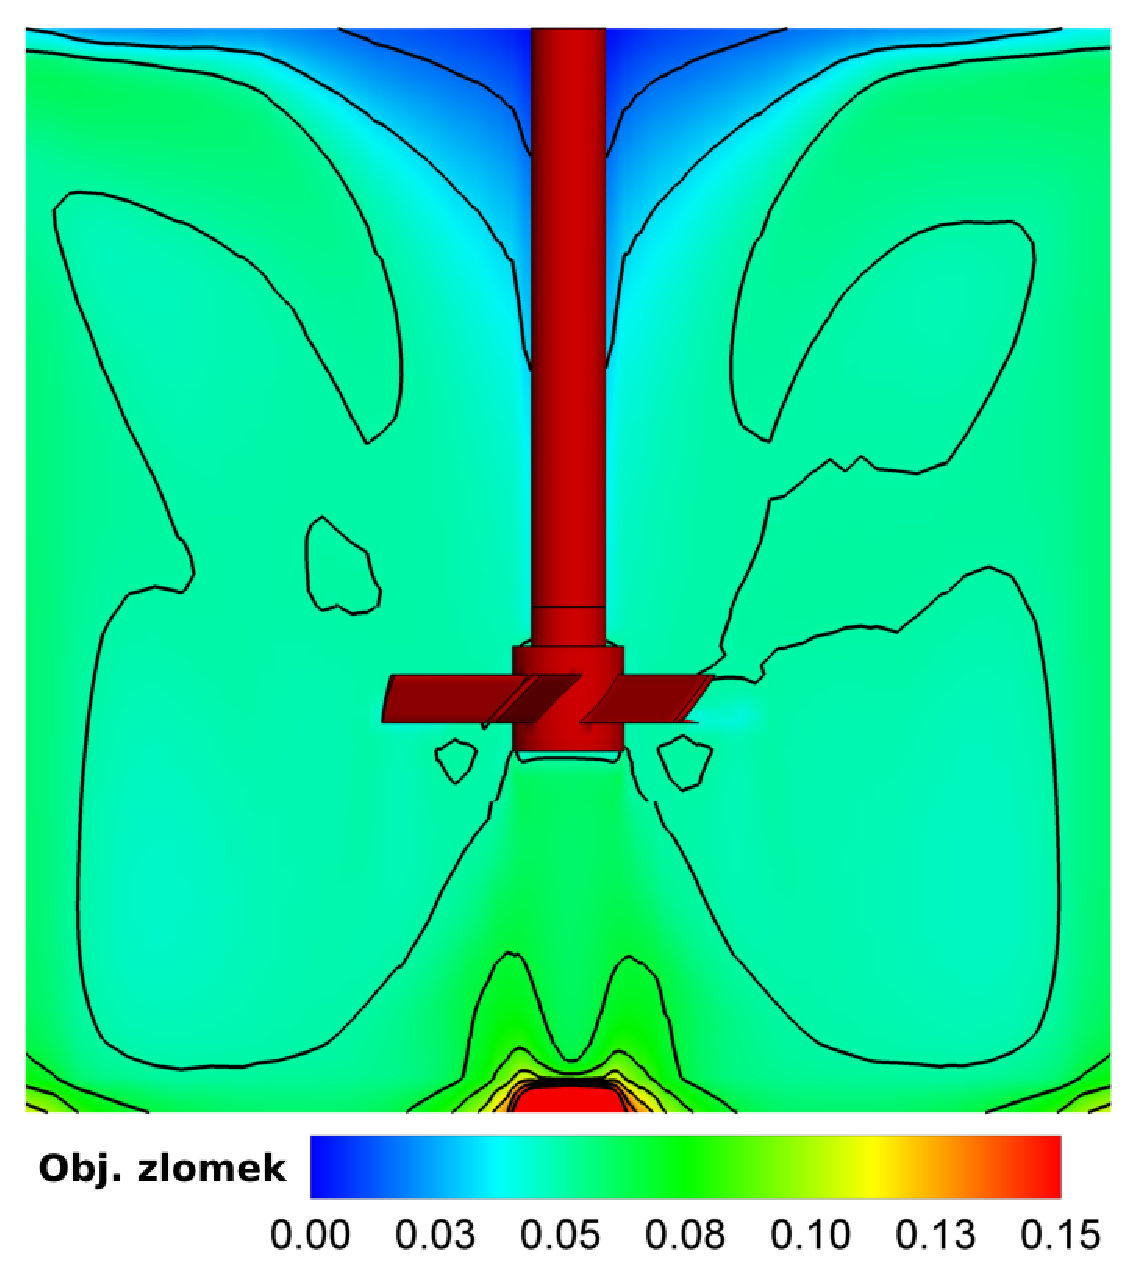
\includegraphics[scale=0.38]{Results/CDComp/kho-7s.eps}}
  \caption{Objemový zlomek pevné fáze v~čase \SI{7}{\second}}
  \label{fig:cd7}
\end{figure}
\newpage
\vspace{-5mm}
Dále jsou zde uvedeny grafické závislosti objemového zlomku pevné fáze na vzdálenosti ode dna nádoby. Z grafu \ref{fig:vol-2} lze vidět, že s~rostoucí vzdáleností se koncentrace pevné fáze postupně snižuje. Avšak grafická závislosti nemá monotonní průběh, přičemž dochází k~tvorbě esovitého koncentračního profilu. Model koeficientu odporu navržený Brucatem předpovídá nižší koncentraci pevné fáze ve vyšší vzdálenosti ode dna než zbylé tři modely. V~čase \SI{7}{\second} kuličky z~PVC již dosáhly značného vznosu a rozdíly mezi jednotlivými korelace pro koeficient odporu se začínaly vytrácet (viz. graf \ref{fig:vol-7}).
\begin{grf}[h!]
 \centering
  \subfloat[v~čase \SI{2}{\second}]{\label{fig:vol-2}\includegraphics[scale=0.39]{Results/CDComp/vol-2s.eps}} 
  \\ 
  \subfloat[v~čase \SI{7}{\second}]{\label{fig:vol-7}\includegraphics[scale=0.39]{Results/CDComp/vol-7s.eps}}
  \caption{Průběh objemového zlomku pevné fáze}
  \label{fig:vol}
\end{grf}
\newpage

Poslední skupina grafů \ref{fig:cd} zachycuje průběh normalizované hodnoty koeficientu odporu v závislosti na světlé výšce. Tato normalizace vznikla vydělením koeficientu odporu jeho průměrnou hodnotou v celé nádrži. Údaje v těchto grafech byly stanoveny podél úsečky v blízkosti radiální narážky.  V~obou případech má  koeficientu odporu podobný průběh pro různé korelace, nicméně v čase \SI{7}{\second} (graf \ref{fig:cd-2}) je zřejmé, že korelace dle Brucata se opět nejznatelněji odlišuje.

\begin{grf}[h!]
 \centering
  \subfloat[v~čase \SI{2}{\second}]{\label{fig:cd-2}\includegraphics[scale=0.40]{Results/CDComp/cd-2s.eps}} 
  \\ 
  \subfloat[v~čase \SI{7}{\second}]{\label{fig:cd-7}\includegraphics[scale=0.40]{Results/CDComp/cd-7s.eps}}
  \caption{Průběh hodnoty koeficientu odporu}
  \label{fig:cd}
\end{grf}
\newpage

\section{Výška vznosu pevné fáze}
Výška suspenzního mraku byla stanovena pro systém tvořený kapalinou \pvpS{} a pevnou fází o koncentraci \volproc{10} při třech různých frekvencí otáčení míchadla. Pro vlastní simulaci byl využit vícefázový přístup Eulerian-Eulerian spolu s Khopkarovým model pro koeficient odporu. Pro potřeby CFD výpočtů \citet{kas08} definovali výšku suspenzního mraku jako vzdálenost mezi dnem nádoby a nejvzdálenějším bodem, který má objemový zlomek zrnité fáze roven průměrné koncentraci v nádrži. Stejný přistup pro učení této výšky byl využit i v následující práci.  

Na obrázku \ref{fig:h-w10-4s-num} je zachycen řez nádobou s konturami objemového zlomku pevné fáze získaný pomocí CFD simulace. Frekvence otáčení míchadla v tomto případě činila \SI{4}{\per\second}. Výška vznosu kuliček z PVC byla, pomocí techniky diskutované výše, stanovena v \SI{24.6}{\centi\meter}. Pro srovnání na obr. \ref{fig:h-w10-4s-exp} je ukázána fotografie pořízená během experimentu. Z ni je dobře patrný vznik rozhraní kapalina-pevná fáze přibližně ve výšce \SI{22}{\centi\meter}, přičemž tato vzdálenost byla stanovena pomocí ocelového metru umístěného od \SI{2}{\centi\meter} nad dnem nádoby.

\begin{figure}[h!]
 \centering
  \subfloat[simulace]{\label{fig:h-w10-4s-num}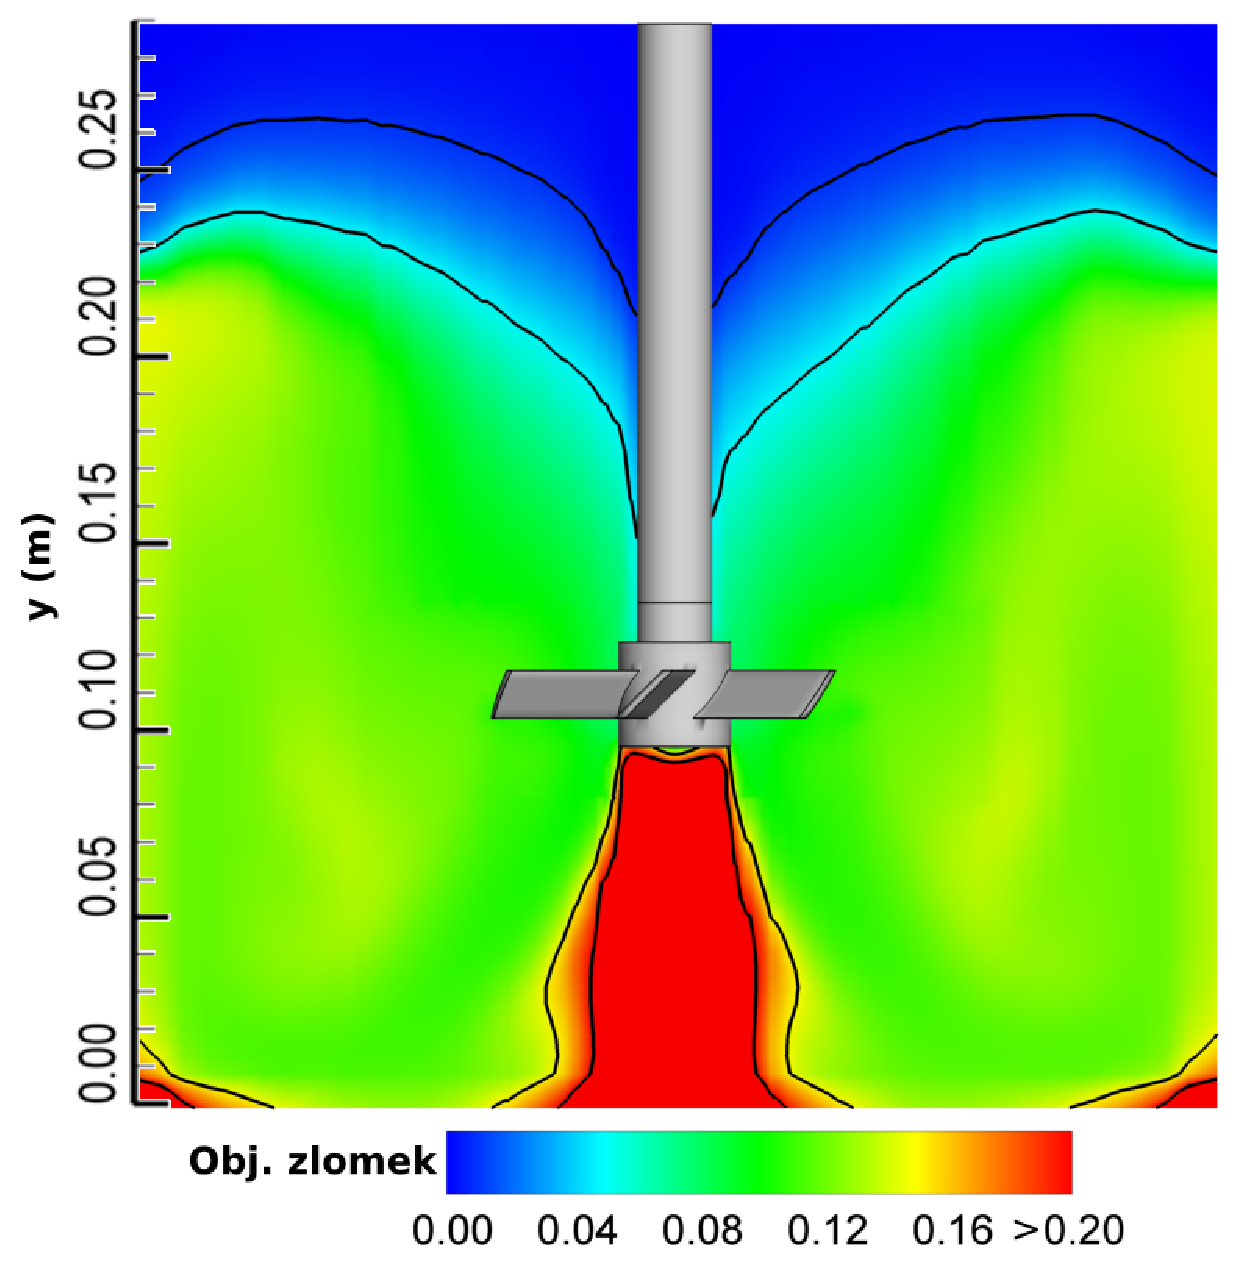
\includegraphics[scale=0.36]{Results/CloudHeight/w10-4s.eps}} 
  \qquad 
  \subfloat[experiment]{\label{fig:h-w10-4s-exp}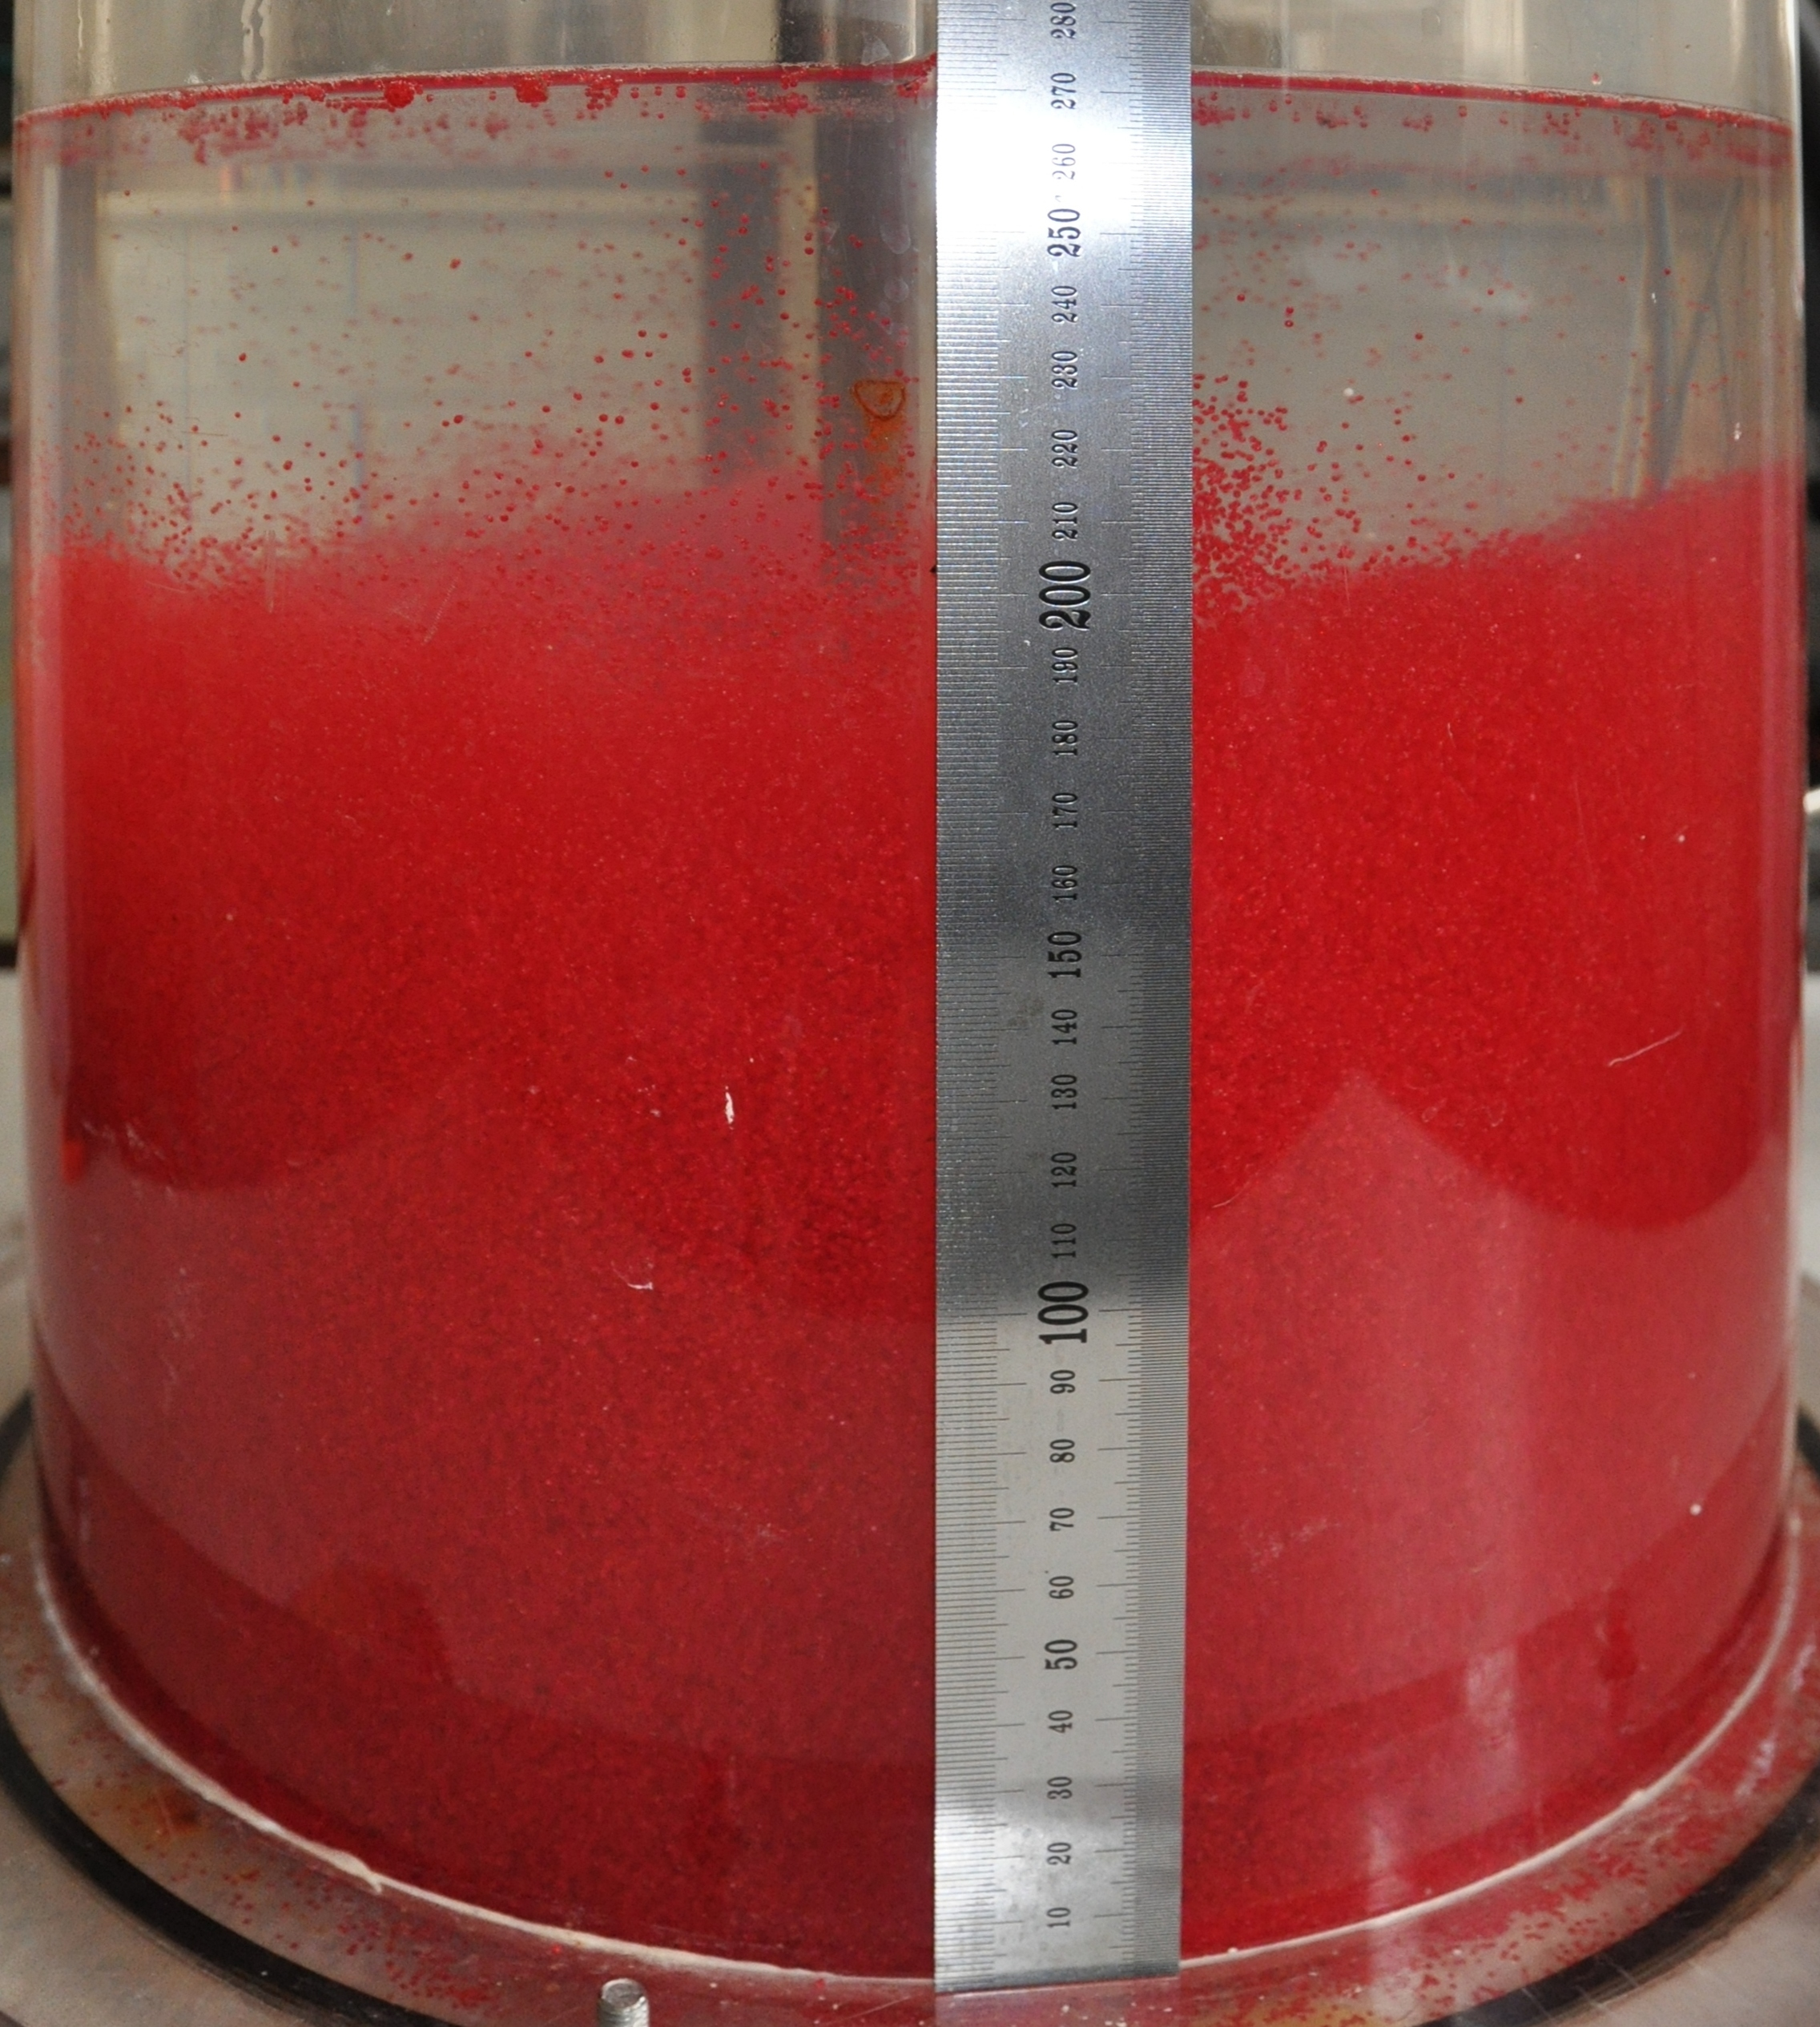
\includegraphics[scale=0.35]{Results/CloudHeight/pvp7-vol10-4s.eps}}
  \caption{Vznos pevné fáze $\kula{N=\SI{4}{\per\second}}$}
  \label{fig:h-w10-4s}
\end{figure}

Vlivem nárůstu rychlosti otáčení míchadla na \SI{5}{\per\second} došlo ke zvýšení výšky suspezního mraku zhruba na \SI{27}{\centi\meter} (viz. obr. \ref{fig:h-w10-5s-exp}). Zmíněný jev byl taktéž pozorován pomocí CFD simulace, což ilustruje řez nádobou \ref{fig:h-w10-5s-num}. Stanovená výška vznosu pevné fáze v tomto případě činila \SI{28.3}{\centi\meter}. 
\newpage

\begin{figure}[t!]
 \centering
  \subfloat[simulace]{\label{fig:h-w10-5s-num}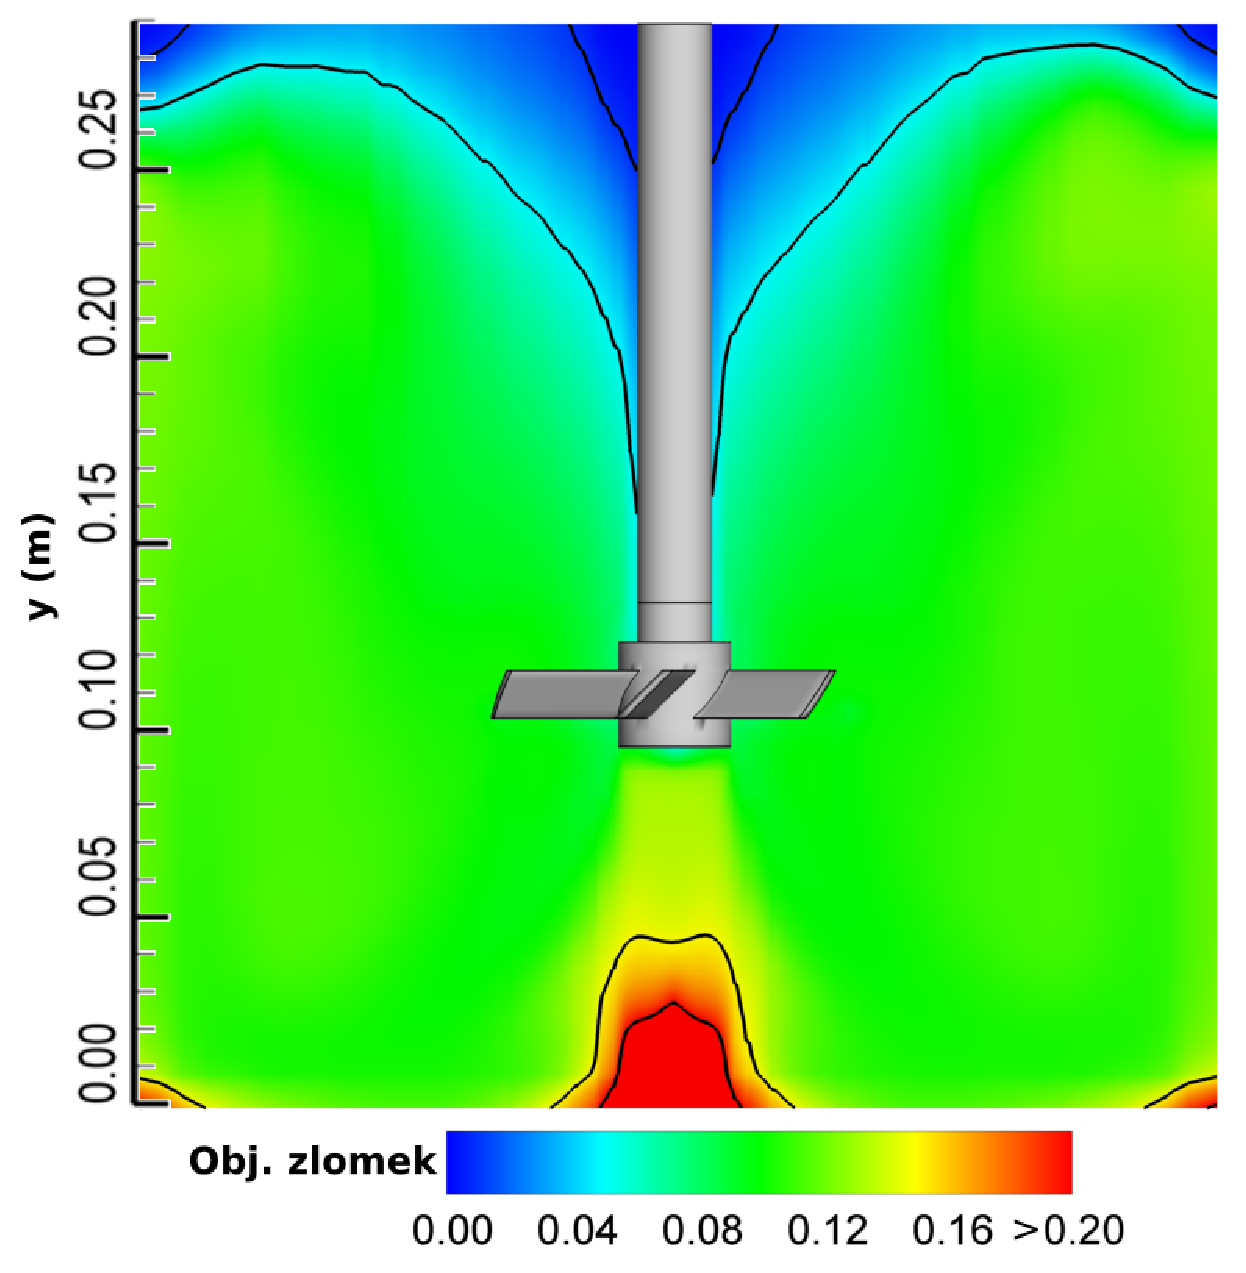
\includegraphics[scale=0.36]{Results/CloudHeight/w10-5s.eps}} 
  \qquad 
  \subfloat[experiment]{\label{fig:h-w10-5s-exp}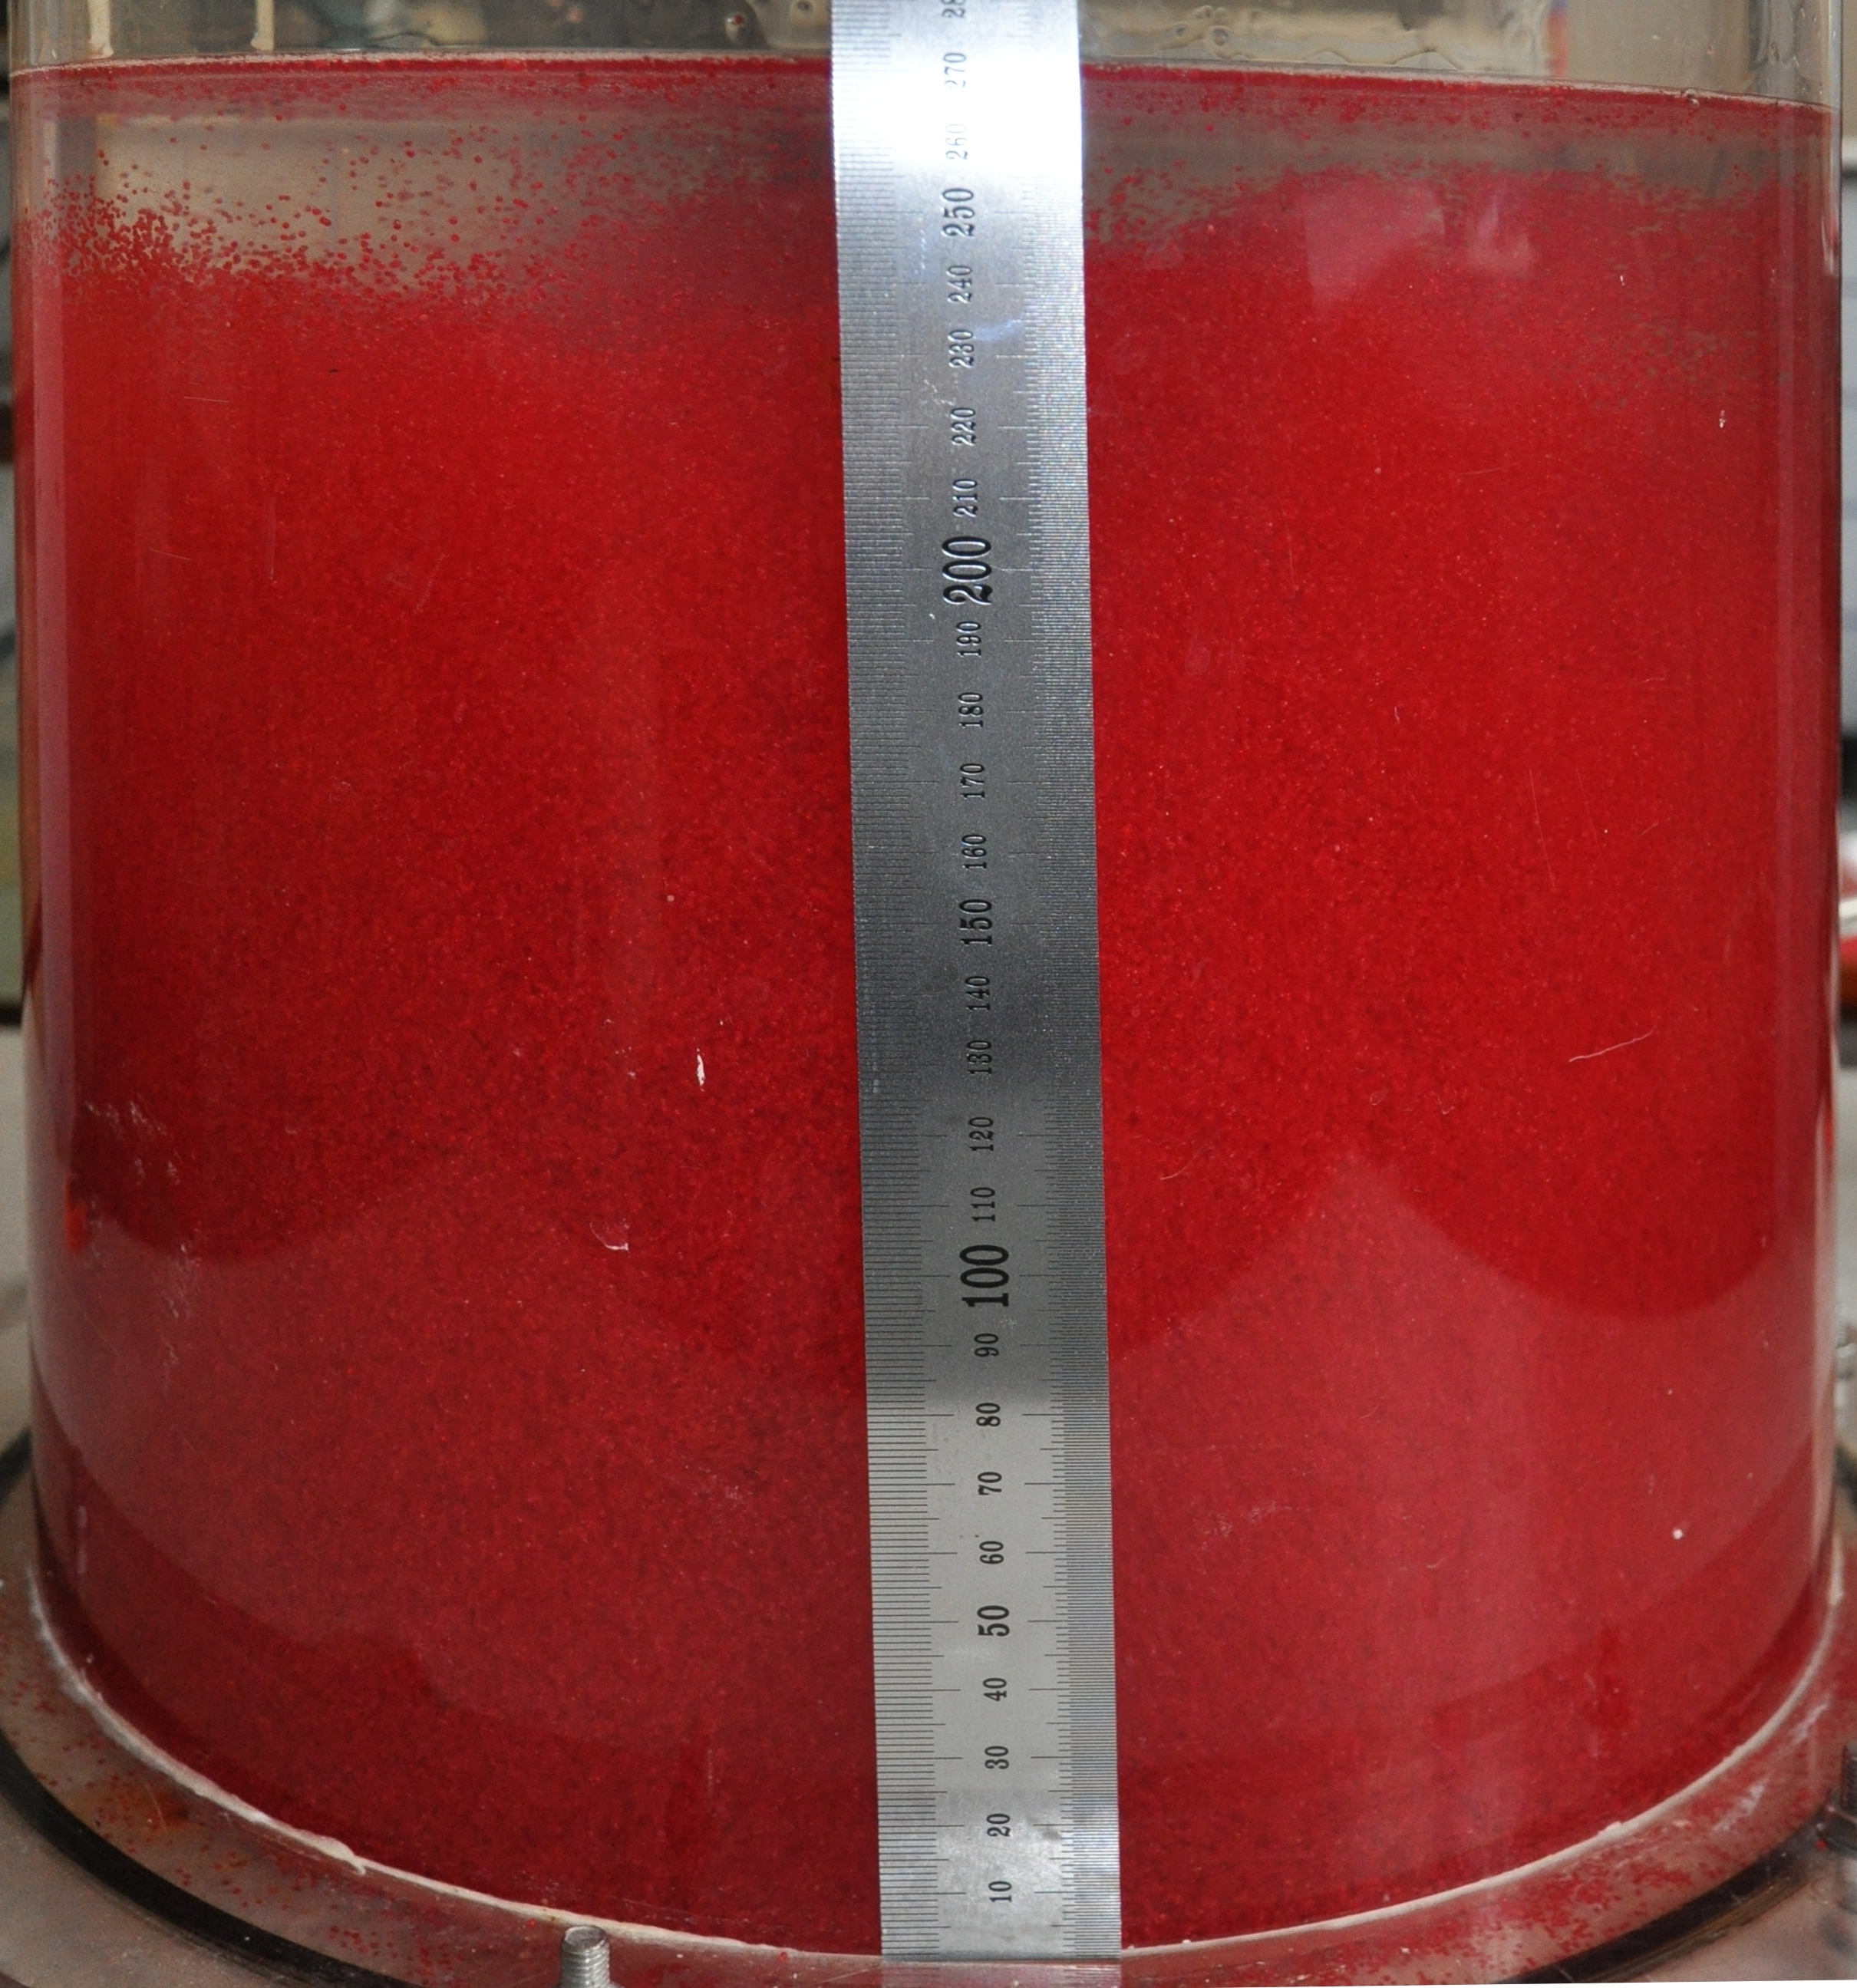
\includegraphics[scale=0.34]{Results/CloudHeight/pvp7-vol10-5s.eps}}
  \caption{Vznos pevné fáze $\kula{N=\SI{5}{\per\second}}$}
  \label{fig:h-w10-5s}
\end{figure}
Poslední skupina obrázků
\begin{figure}[h!]
 \centering
  \subfloat[simulace]{\label{fig:h-w10-6s-num}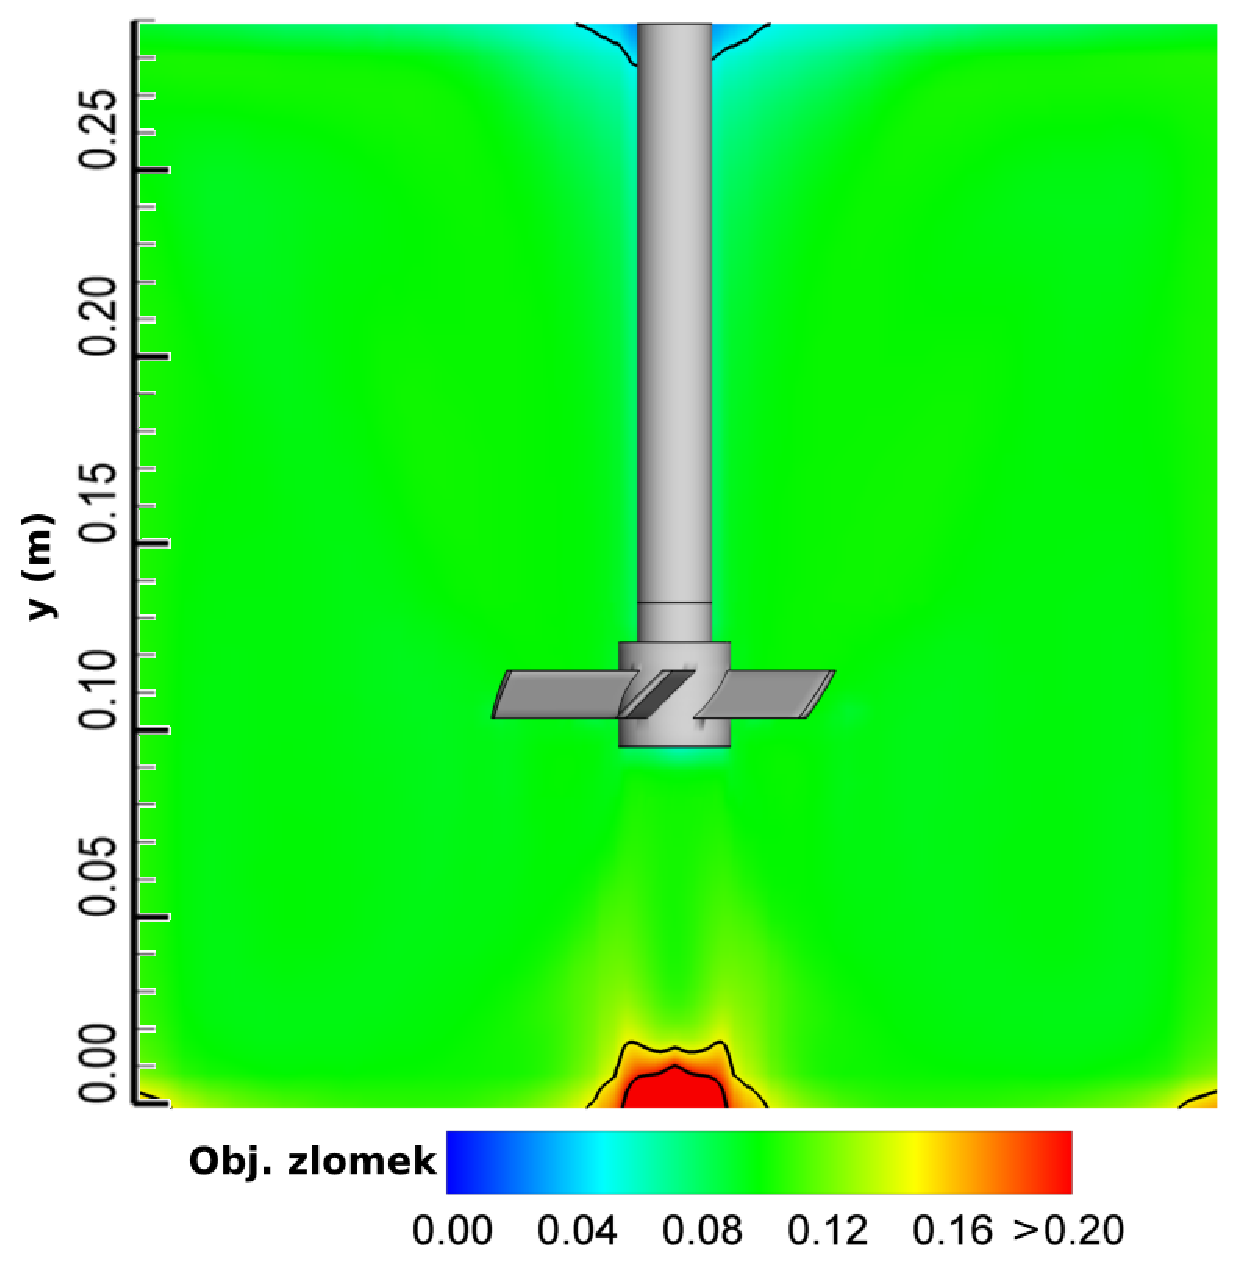
\includegraphics[scale=0.36]{Results/CloudHeight/w10-6s.eps}} 
  \qquad 
  \subfloat[experiment]{\label{fig:h-w10-6s-exp}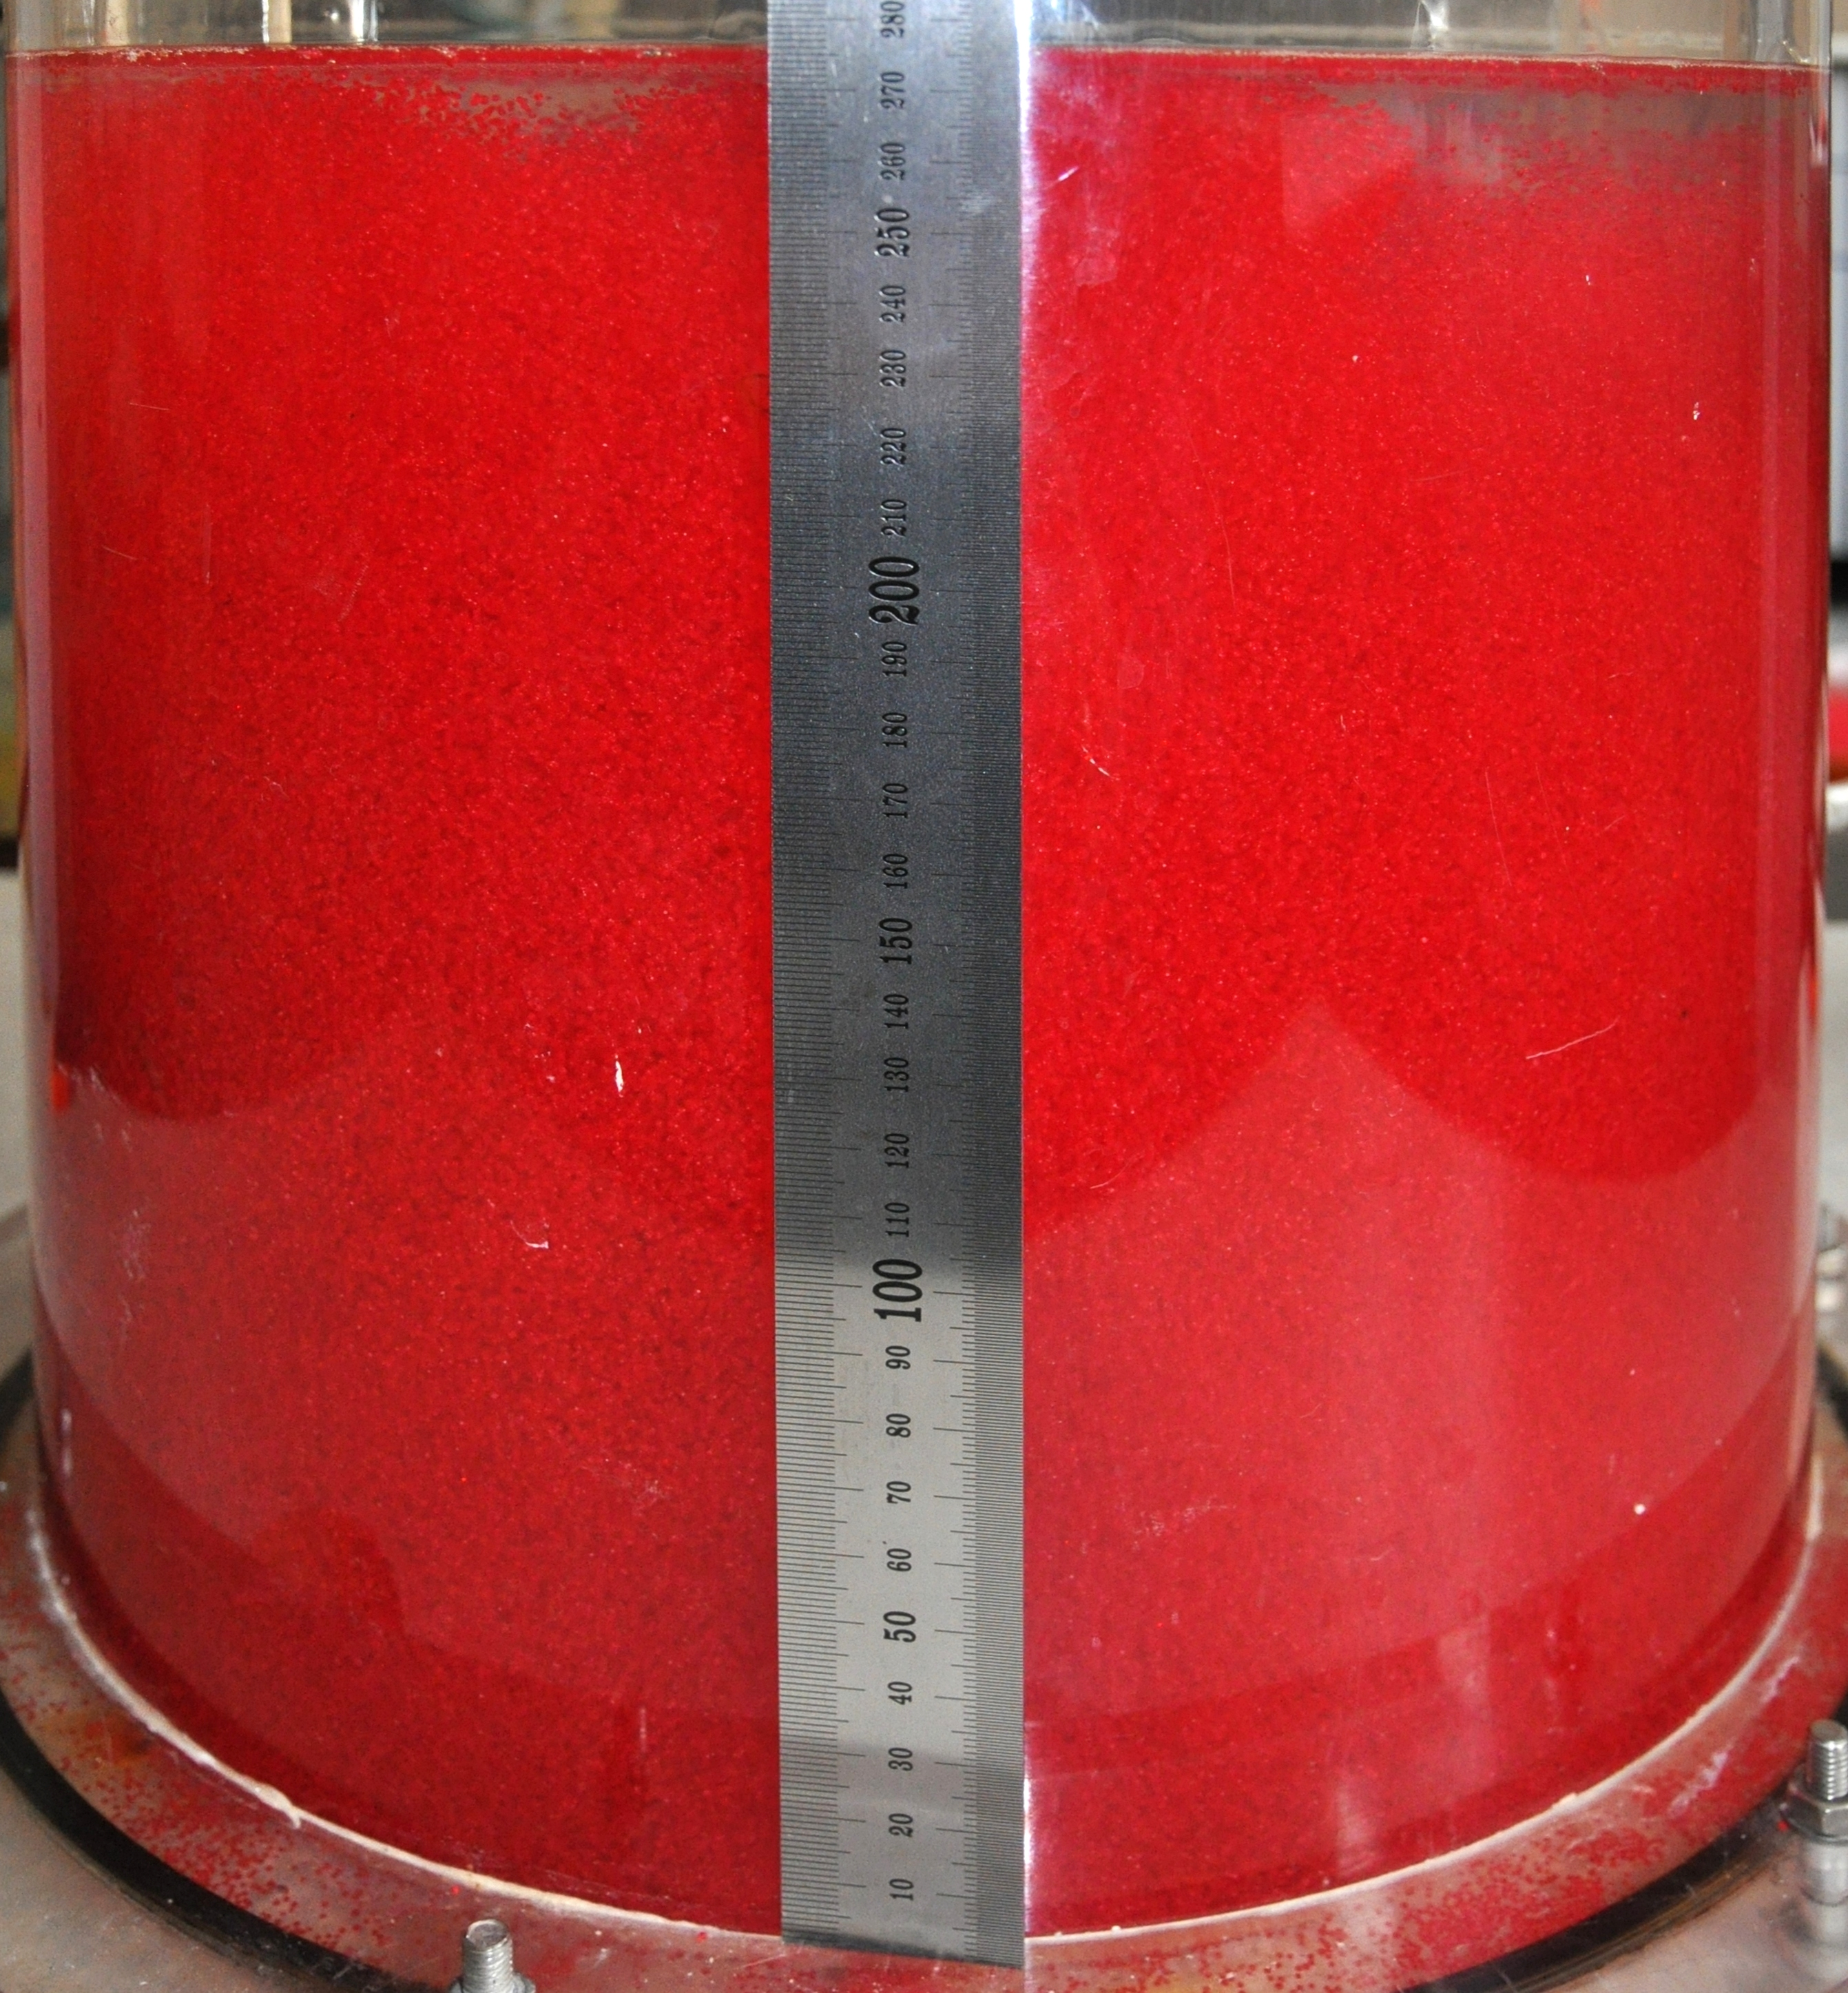
\includegraphics[scale=0.305]{Results/CloudHeight/pvp7-vol10-6s.eps}}
  \caption{Vznos pevné fáze $\kula{N=\SI{6}{\per\second}}$}
  \label{fig:h-w10-6s}
\end{figure}


	\addcontentsline{toc}{chapter}{List of symbols}
\chapter*{List of symbols}

\renewcommand\arraystretch{1.5}
\begin{tabularx}{\textwidth}{@{}p{1.0cm} X r@{}}
$N_{js}$ & just suspended impeller speed & \si{\per\second} \\


\end{tabularx}

\subsubsection*{Greek letters}
\begin{tabularx}{\textwidth}{@{}p{1.0cm} X r@{}}
$N_{js}$ & just suspended impeller speed & \si{\per\second} \\
\end{tabularx}

\subsubsection*{Subscripts}
\begin{tabularx}{\textwidth}{@{}p{1.0cm} X r@{}}
$N_{js}$ & just suspended impeller speed & \si{\per\second} \\
\end{tabularx}

\subsubsection*{Shortcuts}
\begin{tabularx}{\textwidth}{@{}p{1.0cm} X }
CFD & computational fluid dynamics  \\
LDV & laser Doppler velocimetry  \\
\end{tabularx}

	\normalsize{}
	%\setlength{\bibhang}{0pt} odsazen prvního řádku bibliografie
	\begin{thebibliography}{99}
\addcontentsline{toc}{chapter}{Literatura}

\bibitem[Armenante \textit{a kol.}, 1998]{arm98} Armenante, P. M., Nagamine, E. U., Susanto, J., 1998. Determination of correlations to predict the minimum agitation speed for complete solid suspension in agitated vessels. \textit{Can J Chem Eng}, \textbf{76}, 413--419

\bibitem[Baldi \textit{a kol.}, 1978]{bal78} Baldi, G., Conti, R., Alaria, E., 1978. Complete suspension of particles in mechanically agitated vessels. \textit{Chem Eng Sci}, \textbf{33}, 21--25 

\bibitem[Brucato \textit{a kol.}, 1998]{bru98} Brucato, A., Grisafi, F., Montante, G., 1998. Particle drag coefficients in turbulent fluids. \textit{Chem Eng Sci}, \textbf{43}, 3, 3295--3314

\bibitem[Clift \textit{a kol.}, 1978]{cli78} Clift, R., Grace, J. R., Weber, M. E.,  1978.  Bubbles, drops, and particles. \textit{Academic Press}, New York

\bibitem[Derksen, 2003]{derk03} Derksen, J.J., 2003. Numerical Simulation of solid suspension in a stirredtank. \textit{AIChE J}, \textbf{49}, 11, 2700--2714

\bibitem[Gidaspow, 1994]{gid94} Gidaspow, D., 1994. Multiphase flow and fluidization: Continuum and kinematic theory description. \textit{Academic Press}, New York

\bibitem[Hosseini \textit{a kol.}, 2010]{hos10} Hosseini, S., Dineshkumar, P., Ein-Mozaffari, F., Mehrvar, M., 2010. Study of Solid-Liquid Mixing in Agitated Tanks through Computational Fluid Dynamics Modeling \textit{Ind. Eng. Chem. Res.}, \textbf{49}, 4426--4435

\bibitem[Ihme \textit{a kol.}, 1972]{ihme72} Ihme, F., Schmidt-Traub H., Brauer, H., 1972. Theoretische untersuchung \"uber die Umstr\"omung und den Stoff\"ubergang an Kugeln. \textit{Chem Ing Tech}, \textbf{44}, 306

\bibitem[Ishii a Zuber, 1979]{ish79} Ishii, M., Zuber, N., 1979, Drag coefficient and relative velocity in bubbly, droplet or particulate flows. \textit{AIChE J}, \textbf{28}, 843--855 

\bibitem[Kasat \textit{a kol.}, 2008]{kas08} Kasat, G. R., Khopkar, A. R., Ranade, V. V., Pandit, A. B., 2008. CFD Simulation of Liquid-Phase Mixing in Solid-Liquid Stirred Reactor. \textit{Chem Eng Sci}, \textbf{63}, 3877--3885

\bibitem[Khopkar \textit{a kol.}, 2006]{kho06} Khopkar, A. R., Kasat, G. R., Pandit, A. B., Ranade, V. V., 2006. Computational Fluid Dynamics Simulation of Solid Suspension in Stirred Slurry Seactor. \textit{Ind Eng Chem Res} \textbf{45}, 4416--4428.

\bibitem[Kresta a Wood, 1991]{kre91} Kresta, S. M., Wood, P. E., 1991. Prediction of three-dimensional turbulent flow in stirred tanks. \textit{AIChE J}, \textbf{37}, 448--460 

\bibitem[Ljungqvist a Rasmuson, 2001]{lju01} Ljungqvist, M., Rasmuson, A., 2001. Numerical simulation of the two-phase flow in an axially stirred reactor. \textit{Trans AIChE}, \textbf{79}, Part A, 533--546

\bibitem[Micale \textit{a kol.}, 2003]{mic04} Micale, G., Grisafi, F., Rizzuti, L., Brucato, A., 2004. CFD simulation of particle suspension height in stirred vessels. \textit{Chem Eng Res Des}, \textbf{82}, 1204--1213

\bibitem[Micheletti \textit{a kol.}, 2003]{miche03} Micheletti, L., Nikiforaki, L., Lee, K. C., Yianeeskis, M., 2003. Integral and Local Concentration Characteristics of Moderate to Dense Solid-Liquid Suspensions. \textit{11$^{th}$ European Conference on Mixing}, Bamberg, Germany

\bibitem[Montante a Bakker, 2004]{mon04} Montante, G., Bakker, A., 2004, Solid-Liquid Multiphase Flow Validation in Tall Stirred Vessels with Multiple Impeller Systems \textit{Technical Notes}, \textbf{TN253}, Fluent Inc.

\bibitem[např.\ Nienow, 1968]{nie68} Nienow, A. W., 1968. Suspension of solid particles in turbine agitated baffled vessels. \textit{Chem Eng Sci}, \textbf{23}, 1453--1459 

\bibitem[Ochieng a Onyango, 2008]{ochi08} Ochieng, A., Onyango, M. S., 2008. Drag models, solids concentration and velocity distribution in a stirred tank. \textit{Pow Tech}, \textbf{181}, 1--8

\bibitem[Oshinowo a Bakker, 2002]{oshi02} Oshinowo, L. M., Bakker, A., 2002. CFD modeling of solids suspensions in stirred tanks. \textit{Symposium on Computational Modeling of Metals, Minerals and Materials}, February 17-21, Seattle, Washington 

\bibitem[Pinellim \textit{a kol.}, 2001]{pin01} Pinelli, D., Nocentini, M., Magelli, F., 2001. Solids distribution in stirred slurry reactors: in influence of some mixer configurations and limits to the applicability of a simple model for predictions.
\textit{Chem Eng Comm}, \textbf{188}, 91--107

\bibitem[Schiller a Naumann, 1935]{schi32} Schiller, L., Naumann, Z., 1935. A drag coefficient correlation. \textit{Z. Ver. Deutsch. Ing.}, \textbf{77}, 318--320

\bibitem[Syamlalem a O'Brienem, 1993]{syam93} Syamlal, M., O'Brien, T. J., 1993. MFIX Documentation: Theory Guide. \textit{National Technical Information Service}, \textbf{1}, Springfield, Virginia 

\bibitem[Tamburini \textit{a kol.}, 2009]{tamb09} Tamburini, A., Cipollina, A., Micale, G., Ciofalo, M., Brucato, A., 2009. Dense solid–liquid off-bottom suspension dynamics: Simulation and experiment. \textit{Chem Eng Res Des}, \textbf{87}, 587--597

\bibitem[Yamazaki \textit{a kol.}, 2008]{yama08} Yamazaki, H., Tojo, K., Miyanami, K., 1986. Concentration profiles of solids suspended in a stirred tank. \textit{Pow Tech}, \textbf{48}, 205--216

\bibitem[Zwietering, 1957]{zwi58} Zwietering, T. N., 1958. Suspending of solid particles in liquid by agitators. \textit{Chem Eng Sci}, \textbf{8}, 244--253 

\end{thebibliography}

	\chapter*{Příloha}
\label{sec:priloha}
\addcontentsline{toc}{chapter}{Příloha}
Zde jsou uvedeny vytvořené zdrojové kódy uživatelsky definovaných funkcí pro dané modely koeficientu odporu. Online repositář je možné nalézt na adrese:\\ \href{http://code.google.com/p/mixing-udfs/source/browse/\#hg\%2FDragCoefModels}{http://code.google.com/p/mixing-udfs/source/browse/\#hg\%2FDragCoefModels}


\lstinputlisting{Models.c}

\lstinputlisting{SchillerNauman.h}

\end{document}
